%=============================================================================
% EXPERIMENT 3 APPENDIX SECTION (LBA arms) -- copy and paste this whole block.
%
% Self-contained: no custom macros, no \input, nothing to define elsewhere.
%
% Requires in your preamble:
%   \usepackage{graphicx}
%   \usepackage{booktabs}
%   \usepackage{placeins}   % for \FloatBarrier
%
% Figure paths are relative to this directory (outputs/finals/experiment-3/),
% i.e. "zeroshot/lba/<case>/<plot>.pdf" and "finetuned/lba/<case>/<plot>.pdf".
% If the main document moves, find-and-replace the prefixes "zeroshot/" and
% "finetuned/" throughout this block.
%
% Source: frozen experiment-3 snapshot, assembled 2026-09-02 by
% experiments/finalize_experiment_3.py at git commit c9d6f970.
% See README.md, paired_validation_notes.md and MANIFEST.csv.
%=============================================================================

% --- Float placement: these panels are large. Defaults restored at the end of
% --- this block, so pasting it mid-document does not affect other sections.
\renewcommand{\topfraction}{0.92}
\renewcommand{\bottomfraction}{0.7}
\renewcommand{\textfraction}{0.06}
\renewcommand{\floatpagefraction}{0.6}

%=============================================================================
\section{Experiment 3: LBA zero-shot and finetuned recovery}
\label{app:experiment-3-lba-figures}
%=============================================================================

This appendix collects the per-condition diagnostic panels for the linear
ballistic accumulator (LBA), a family the model-class CogFormer was \emph{not}
trained on. Two arms are shown for every condition: the \emph{zero-shot} arm
applies the original pre-finetune checkpoint to LBA data directly, and the
\emph{finetuned} arm applies the LBA-finetuned checkpoint. Both arms are
evaluated on the same paired validation data, so the two panels of a given
condition differ only in the checkpoint that produced them.

For each of the six design conditions listed in
Table~\ref{tab:e3-lba-conditions} we report two diagnostics per arm:
\emph{coefficient recovery} (posterior mean and 95\% credible interval against
ground truth) and \emph{ECDF calibration} (rank-based simulation-based
calibration, plotted as the difference from the uniform diagonal with
simultaneous 95\% bands). This gives $6 \times 2 \times 2 = 24$ panels. Within
each condition the two arms are placed adjacently for the same diagnostic, so
that the zero-shot and finetuned versions of a panel can be compared directly.

LBA intrinsic parameters are the base drift $v$, the drift advantage
$v_{\mathrm{diff}}$ for the favored accumulator, the threshold $a$, the
non-decision time $\tau$, and the dispersions $s_v, s_\tau$. As elsewhere, the
panels cover the \emph{local} coefficient matrix only: the global contamination
probability $\pi$ is estimated jointly but scored and plotted separately, and
its panels are omitted here. Empirical coverage and the NRMSE/contraction/
calibration-error heatmaps are also produced for every condition but not
reproduced; their values are tabulated in the per-condition
\texttt{metrics.csv} files.

Table~\ref{tab:e3-lba-nrmse} gives the headline summary the panels visualize:
mean NRMSE per condition in each arm. Finetuning reduces LBA error in every
condition, by $48.2\%$ overall.

\begin{table}[htbp]
  \centering
  \small
  \begin{tabular}{@{}llp{7.0cm}@{}}
    \toprule
    \# & Condition & Design \\
    \midrule
    1 & Intercept-only    & Intercept row only; all intrinsic parameters free,
                            no regressors. \\
    2 & Regressed         & Intercept plus two continuous main-effect
                            regressors $u_1, u_2$; no interaction. \\
    3 & Fixed-regressed   & As \emph{regressed}, but with the dispersion
                            parameters $s_v, s_\tau$ held fixed. \\
    4 & Interaction       & Intercept, both main effects, and the
                            $u_1{:}u_2$ interaction, with hierarchical
                            shedding of parameters across blocks. \\
    5 & Fixed             & Intercept-only with $s_v, s_\tau$ held fixed. \\
    6 & Mixed-predictor   & Interaction design with $u_1$ categorical (at the
                            training-maximum number of categories) and $u_2$
                            continuous, i.e.\ a categorical~$\times$~continuous
                            interaction. \\
    \bottomrule
  \end{tabular}
  \caption{The six validation design conditions, in the order used throughout
    this appendix. These are the same conditions used for the trained families.}
  \label{tab:e3-lba-conditions}
\end{table}

\begin{table}[htbp]
  \centering
  \small
  \begin{tabular}{@{}lrrr@{}}
    \toprule
    Condition & Zero-shot & Finetuned & Change \\
    \midrule
    Intercept-only   & 0.3424 & 0.1457 & $-0.1967$ \\
    Regressed        & 0.2617 & 0.0846 & $-0.1771$ \\
    Fixed-regressed  & 0.3076 & 0.0499 & $-0.2577$ \\
    Interaction      & 0.1838 & 0.0989 & $-0.0849$ \\
    Fixed            & 0.4153 & 0.1376 & $-0.2778$ \\
    Mixed-predictor  & 0.2054 & 0.1601 & $-0.0453$ \\
    \midrule
    \textbf{Overall} & \textbf{0.2386} & \textbf{0.1237} & $\mathbf{-48.2\%}$ \\
    \bottomrule
  \end{tabular}
  \caption{LBA mean NRMSE per design condition, aggregated over the active
    parameter rows of each condition's \texttt{metrics.csv} (80 LBA rows per
    arm). Lower is better. Note that the underlying RMSE estimator is
    stochastic at the $1$--$2\%$ level, so differences of that size should not
    be read as meaningful; the reductions here are an order of magnitude
    larger.}
  \label{tab:e3-lba-nrmse}
\end{table}

\paragraph{A note on interaction row labels.}
In the LBA panels the interaction block is labelled positionally --- as $u_5$
in the \emph{interaction} condition, and as $u_5, u_6, u_7$ in the
\emph{mixed-predictor} condition --- rather than by the terms it represents.
The equivalent panels for the trained families label these same rows
$u_1 \times u_2$ and $u_1{:}c_k \times u_2$. The row layout, ordering and block
sizes are identical; only the axis text differs, so $u_5$ in
Figures~\ref{fig:e3-lba-interaction-zeroshot-rec}
and~\ref{fig:e3-lba-interaction-finetuned-rec} should be read as
$u_1 \times u_2$, and $u_5, u_6, u_7$ in
Figures~\ref{fig:e3-lba-mixed_predictor-zeroshot-rec}
and~\ref{fig:e3-lba-mixed_predictor-finetuned-rec} as
$u_1{:}c_1 \times u_2$, $u_1{:}c_2 \times u_2$ and $u_1{:}c_3 \times u_2$.

\FloatBarrier
\clearpage

%-----------------------------------------------------------------------------
\subsection{LBA, intercept-only design}
\label{sec:e3-lba-intercept_only}
%-----------------------------------------------------------------------------

\begin{figure}[htbp]
  \centering
  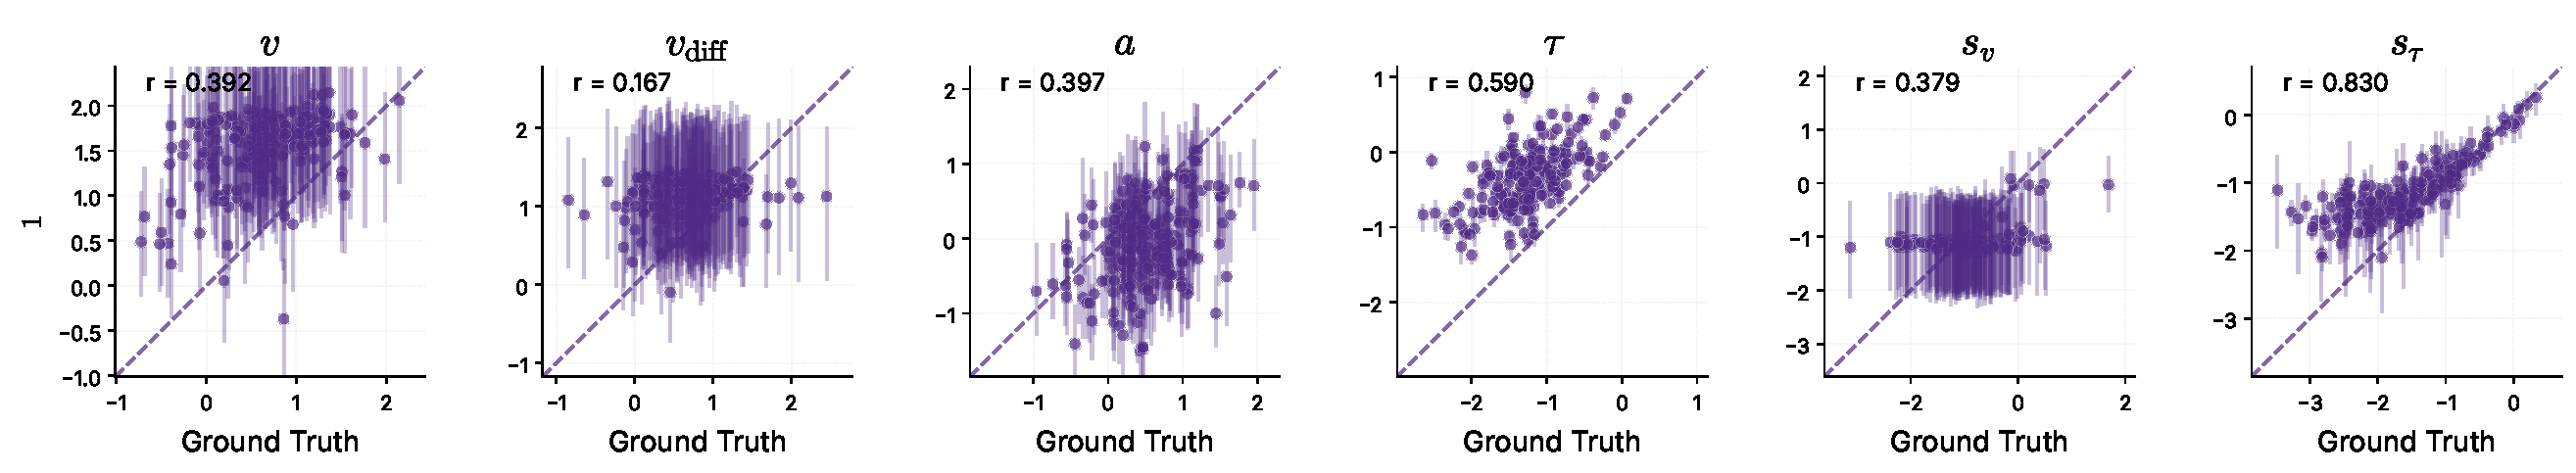
\includegraphics[width=\linewidth,height=0.84\textheight,keepaspectratio]{zeroshot/lba/intercept_only/recovery.pdf}
  \caption[LBA, intercept-only, zero-shot: recovery]{\textbf{LBA, intercept-only design, zero-shot --- coefficient recovery.} Posterior mean (points) with 95\% credible intervals against the
    data-generating value, one panel per active cell of the coefficient matrix
    $\mathbf{B}$. Columns are intrinsic parameters, rows are design columns
    (intercept, main effects, interactions), labeled by regressor and category;
    the panel axes render this as \texttt{predictor|category}. Inactive cells are
    drawn as grey N/A tiles. Point color encodes the row kind: intercept (purple),
    main effect (blue), interaction (red). This arm evaluates the original pre-finetune checkpoint applied to LBA without any LBA training.}
  \label{fig:e3-lba-intercept_only-zeroshot-rec}
\end{figure}

\begin{figure}[htbp]
  \centering
  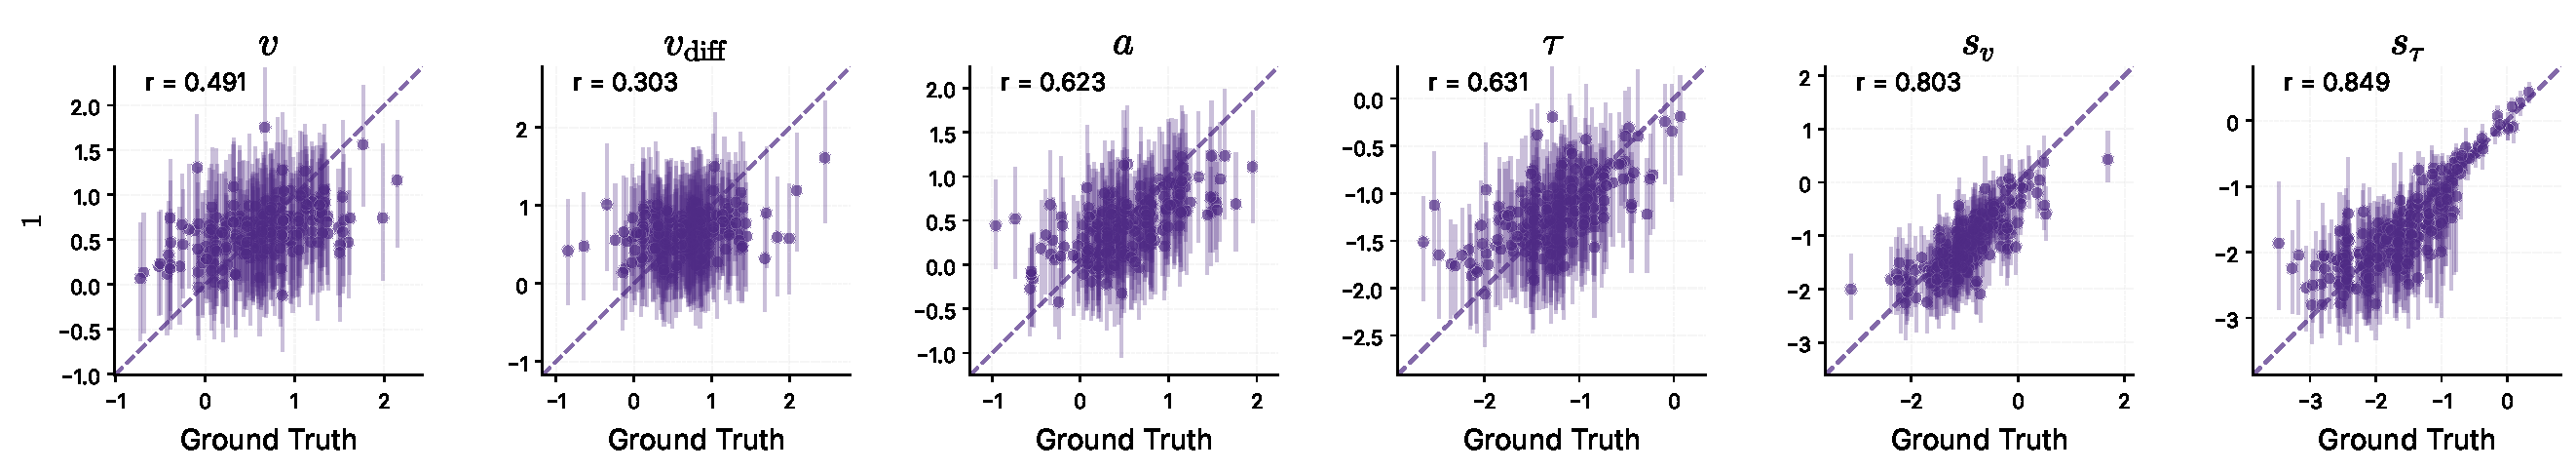
\includegraphics[width=\linewidth,height=0.84\textheight,keepaspectratio]{finetuned/lba/intercept_only/recovery.pdf}
  \caption[LBA, intercept-only, finetuned: recovery]{\textbf{LBA, intercept-only design, finetuned --- coefficient recovery.} Posterior mean (points) with 95\% credible intervals against the
    data-generating value, one panel per active cell of the coefficient matrix
    $\mathbf{B}$. Columns are intrinsic parameters, rows are design columns
    (intercept, main effects, interactions), labeled by regressor and category;
    the panel axes render this as \texttt{predictor|category}. Inactive cells are
    drawn as grey N/A tiles. Point color encodes the row kind: intercept (purple),
    main effect (blue), interaction (red). This arm evaluates the LBA-finetuned checkpoint.}
  \label{fig:e3-lba-intercept_only-finetuned-rec}
\end{figure}

\begin{figure}[htbp]
  \centering
  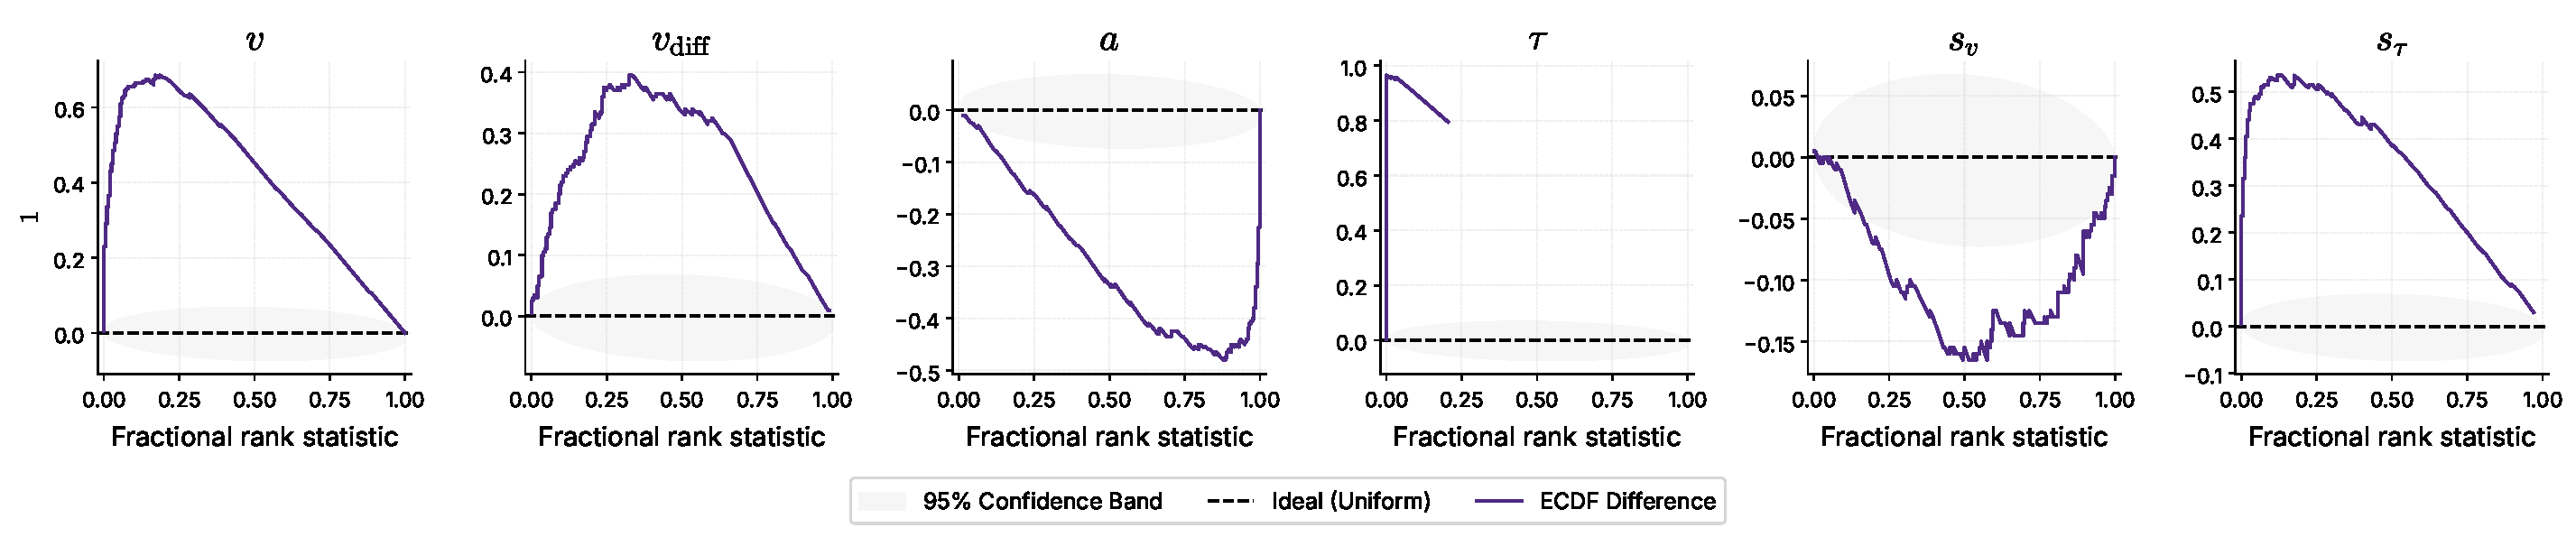
\includegraphics[width=\linewidth,height=0.84\textheight,keepaspectratio]{zeroshot/lba/intercept_only/ecdf.pdf}
  \caption[LBA, intercept-only, zero-shot: ECDF calibration]{\textbf{LBA, intercept-only design, zero-shot --- ECDF calibration.} Rank-ECDF difference (empirical minus uniform) with simultaneous
    95\% confidence bands, on the same cell layout as the corresponding recovery
    figure (Figure~\ref{fig:e3-lba-intercept_only-zeroshot-rec}). A calibrated posterior stays inside the band;
    excursions above/below indicate bias, and a systematically shallow/steep curve
    indicates over-/under-dispersion.}
  \label{fig:e3-lba-intercept_only-zeroshot-ecdf}
\end{figure}

\begin{figure}[htbp]
  \centering
  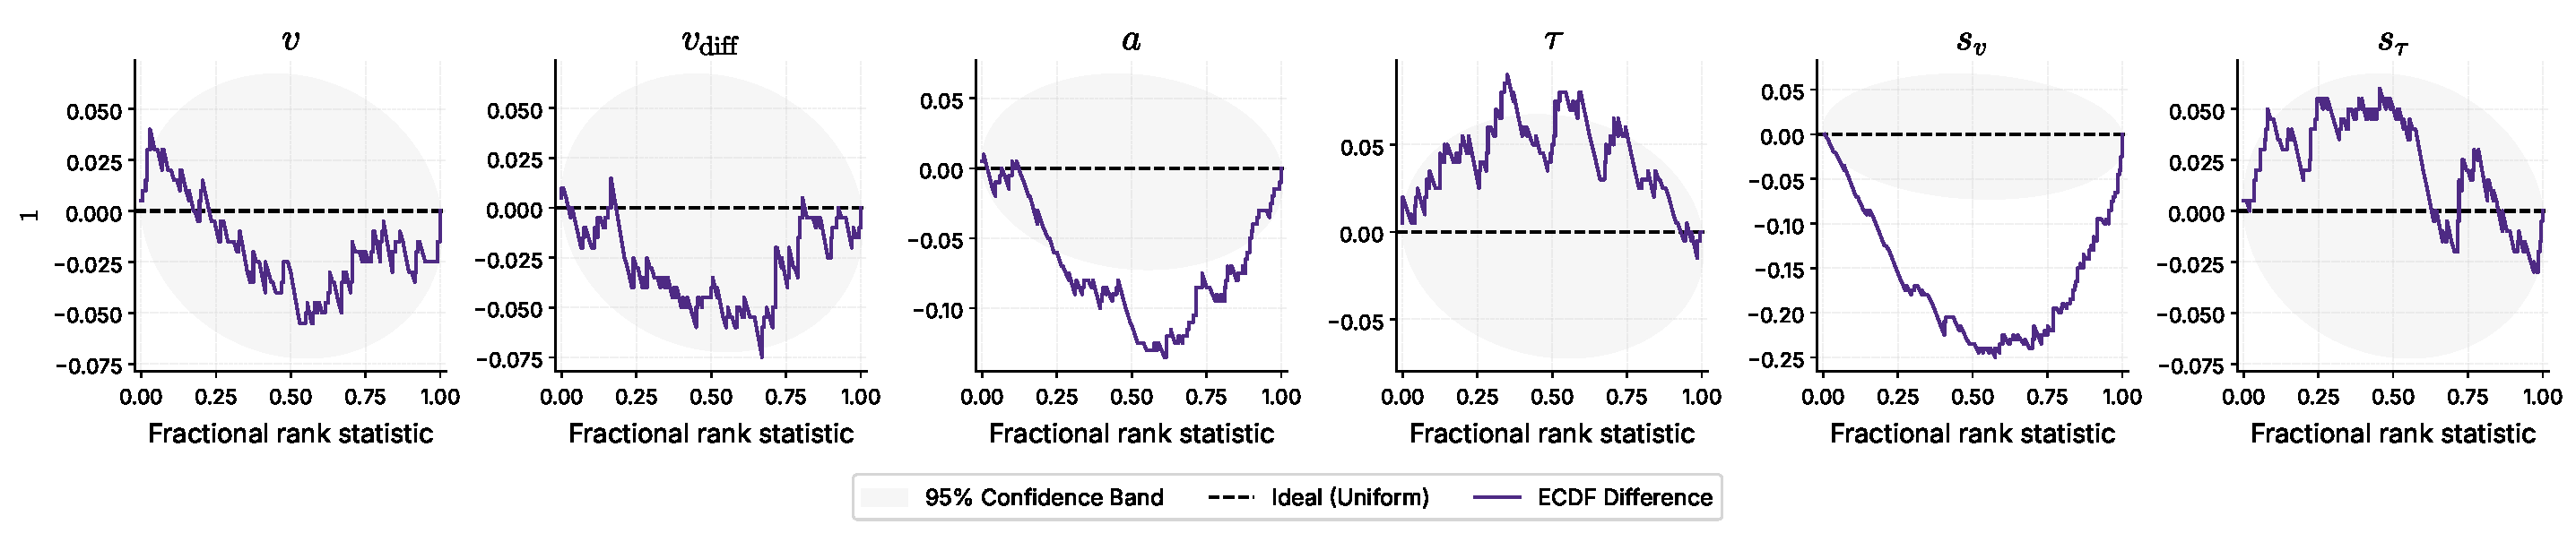
\includegraphics[width=\linewidth,height=0.84\textheight,keepaspectratio]{finetuned/lba/intercept_only/ecdf.pdf}
  \caption[LBA, intercept-only, finetuned: ECDF calibration]{\textbf{LBA, intercept-only design, finetuned --- ECDF calibration.} Rank-ECDF difference (empirical minus uniform) with simultaneous
    95\% confidence bands, on the same cell layout as the corresponding recovery
    figure (Figure~\ref{fig:e3-lba-intercept_only-finetuned-rec}). A calibrated posterior stays inside the band;
    excursions above/below indicate bias, and a systematically shallow/steep curve
    indicates over-/under-dispersion.}
  \label{fig:e3-lba-intercept_only-finetuned-ecdf}
\end{figure}

\FloatBarrier
\clearpage

%-----------------------------------------------------------------------------
\subsection{LBA, regressed design}
\label{sec:e3-lba-regressed}
%-----------------------------------------------------------------------------

\begin{figure}[htbp]
  \centering
  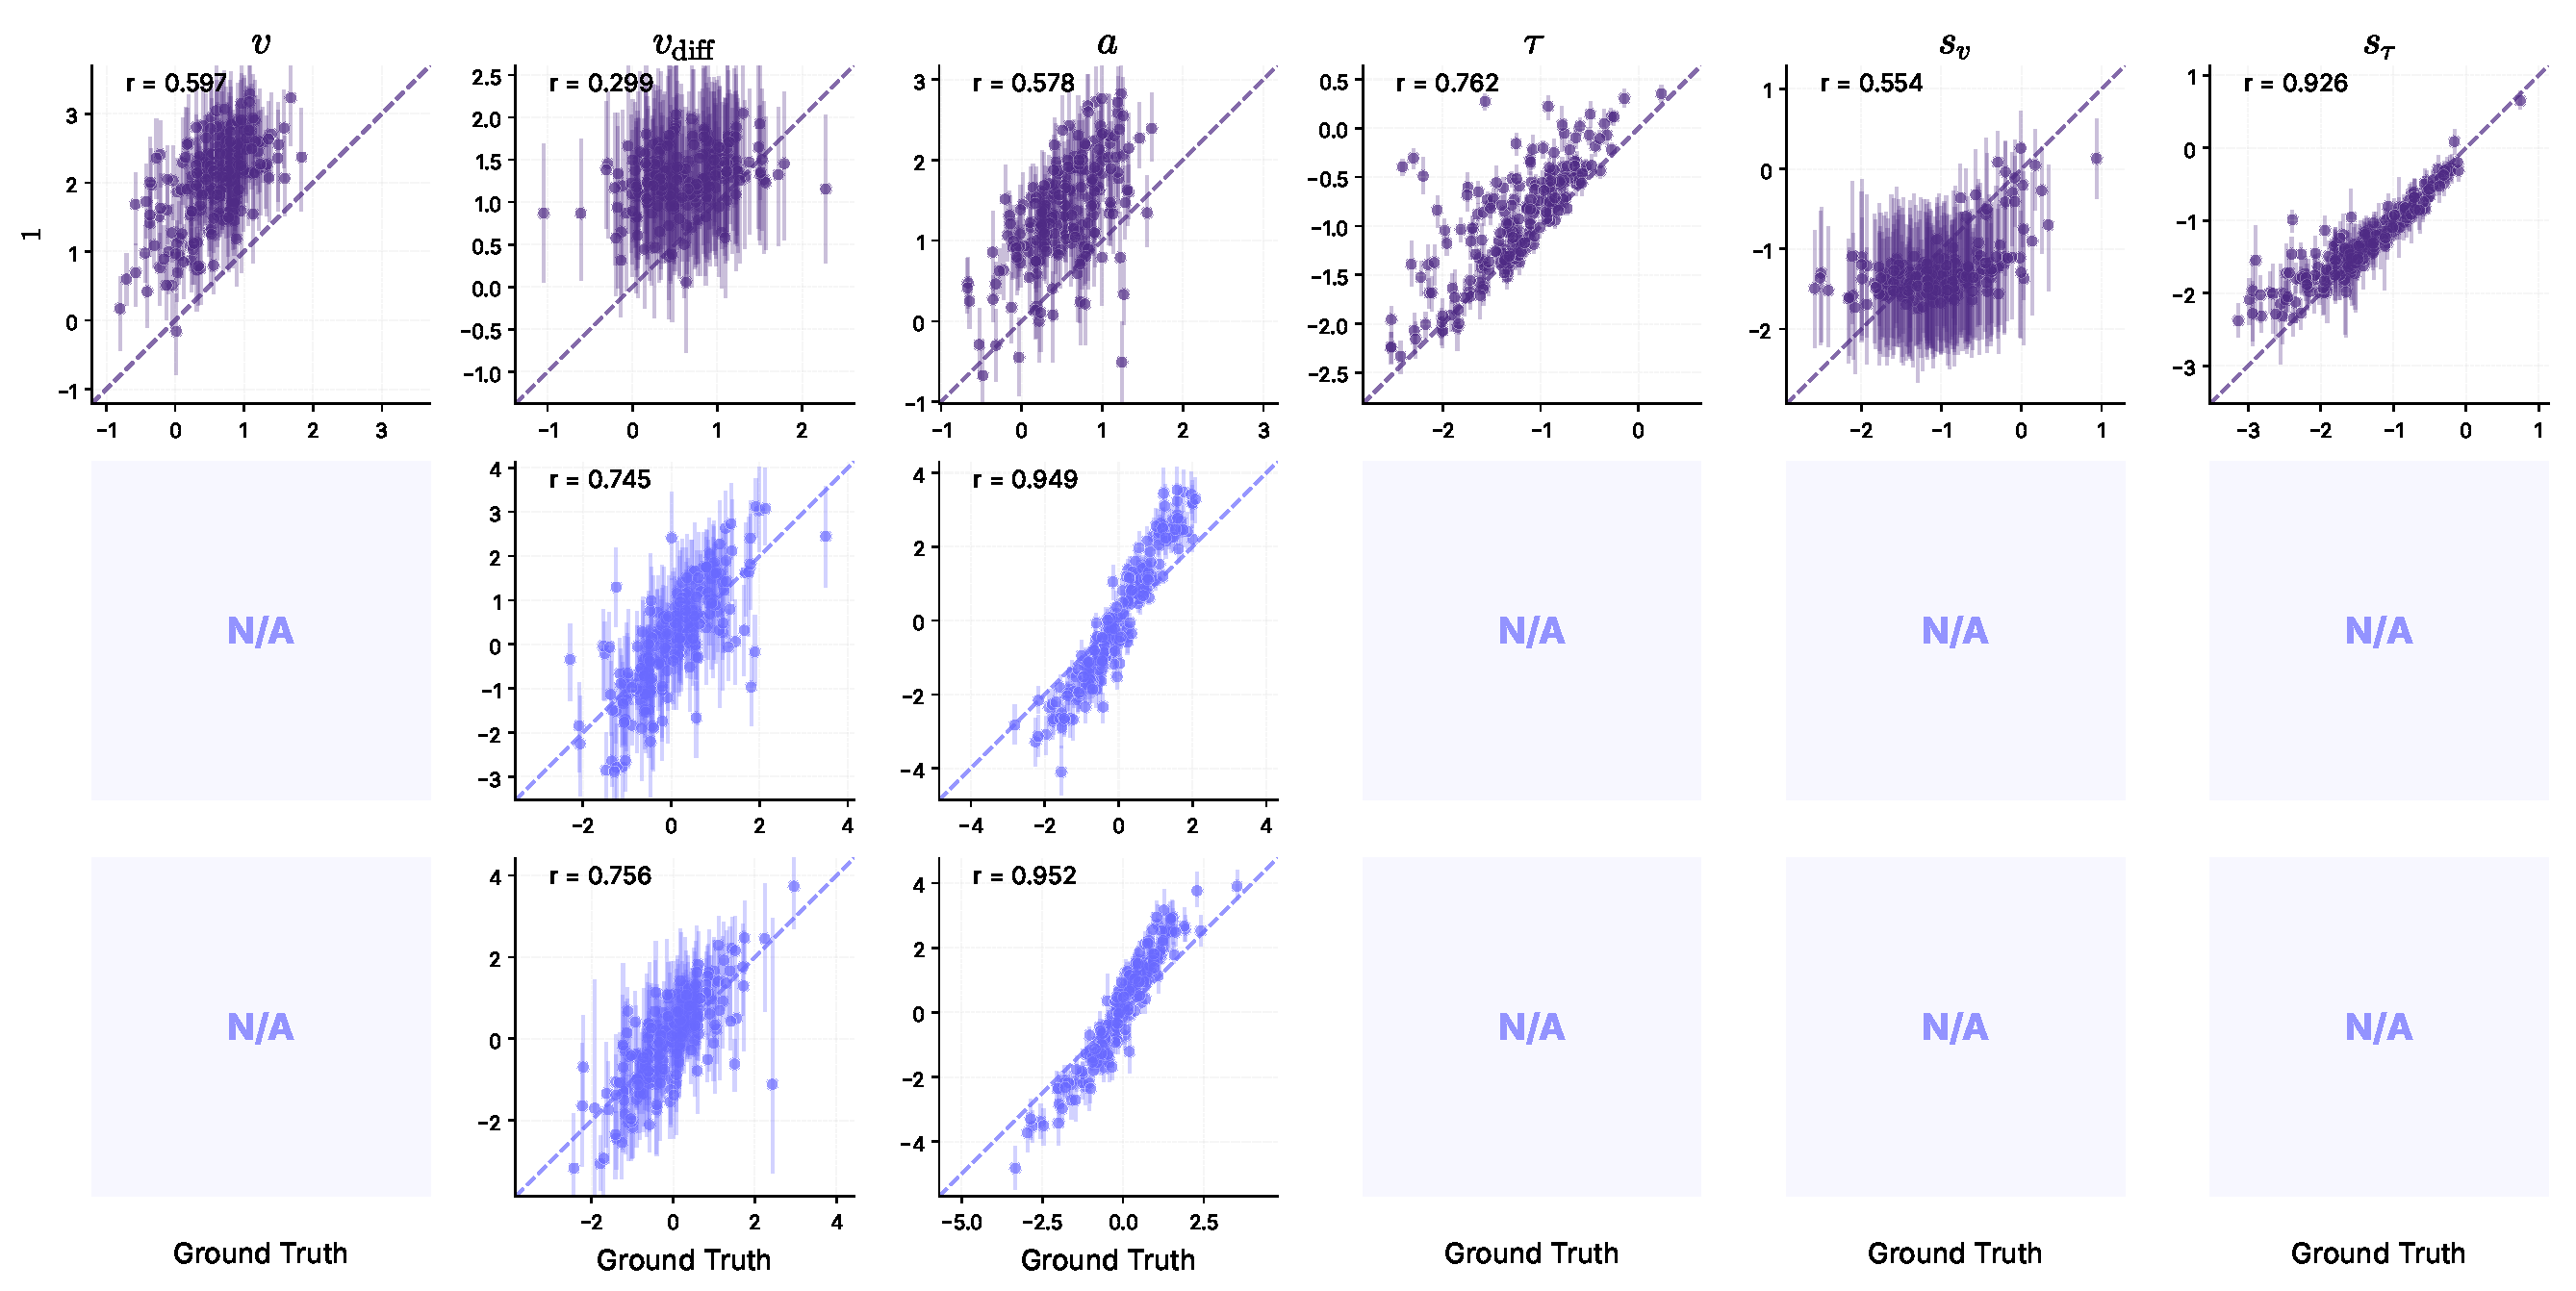
\includegraphics[width=\linewidth,height=0.84\textheight,keepaspectratio]{zeroshot/lba/regressed/recovery.pdf}
  \caption[LBA, regressed, zero-shot: recovery]{\textbf{LBA, regressed design, zero-shot --- coefficient recovery.} Posterior mean (points) with 95\% credible intervals against the
    data-generating value, one panel per active cell of the coefficient matrix
    $\mathbf{B}$. Columns are intrinsic parameters, rows are design columns
    (intercept, main effects, interactions), labeled by regressor and category;
    the panel axes render this as \texttt{predictor|category}. Inactive cells are
    drawn as grey N/A tiles. Point color encodes the row kind: intercept (purple),
    main effect (blue), interaction (red). This arm evaluates the original pre-finetune checkpoint applied to LBA without any LBA training.}
  \label{fig:e3-lba-regressed-zeroshot-rec}
\end{figure}

\begin{figure}[htbp]
  \centering
  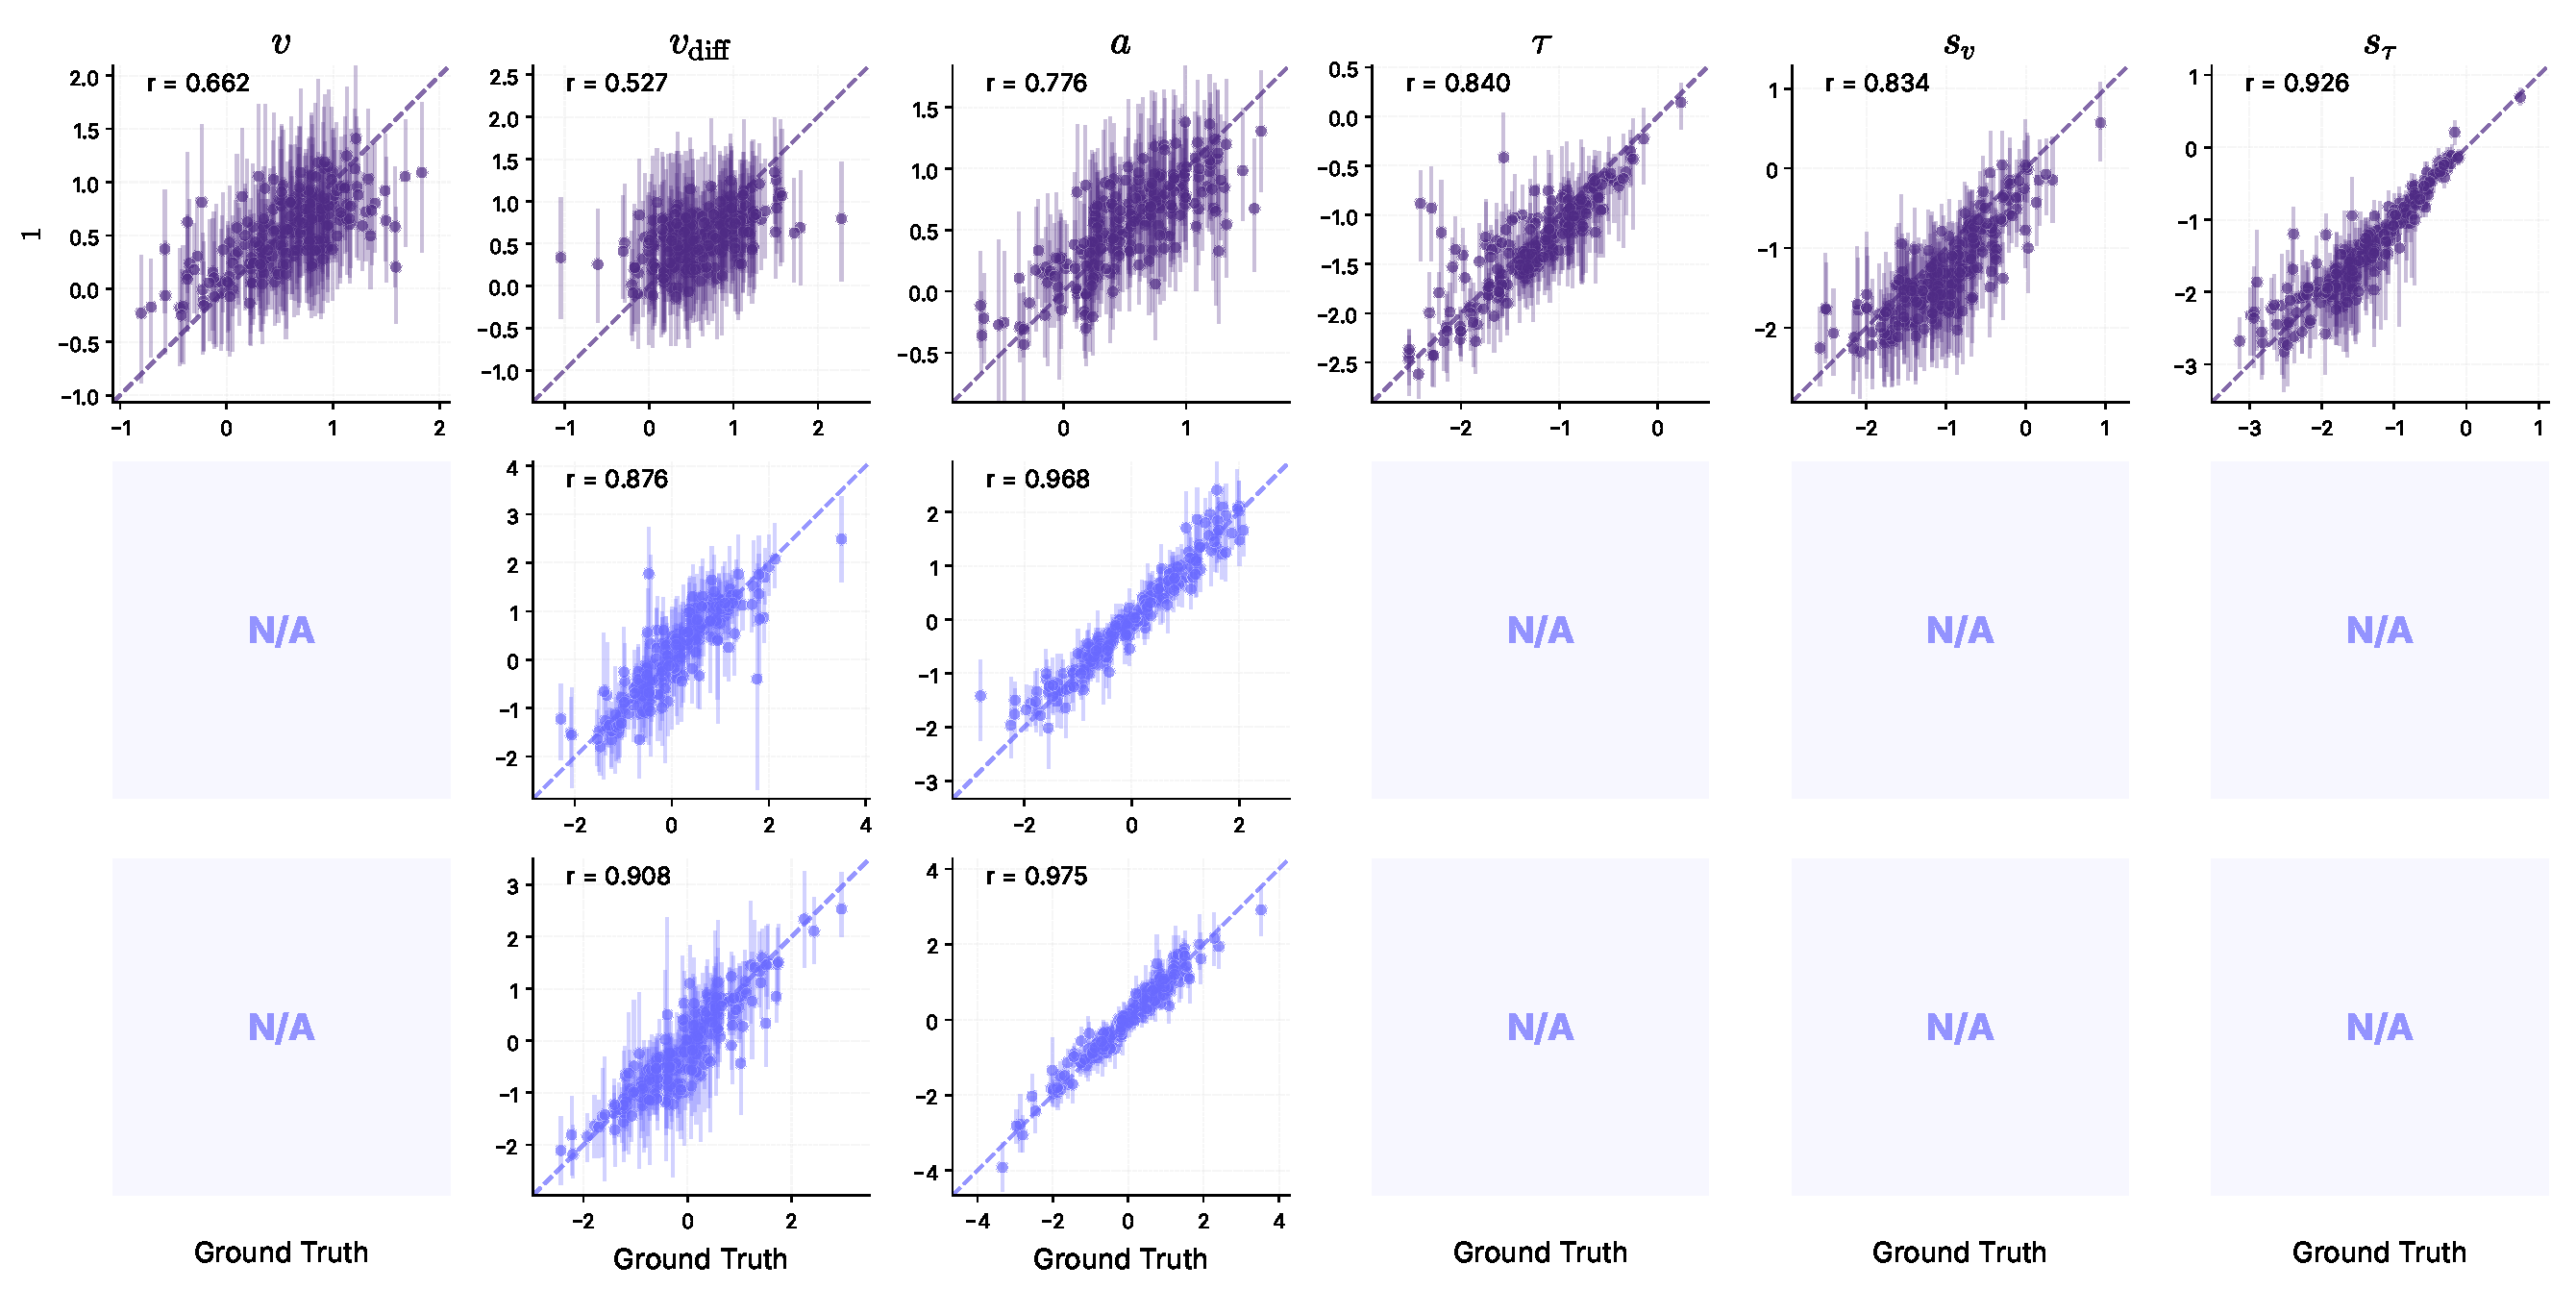
\includegraphics[width=\linewidth,height=0.84\textheight,keepaspectratio]{finetuned/lba/regressed/recovery.pdf}
  \caption[LBA, regressed, finetuned: recovery]{\textbf{LBA, regressed design, finetuned --- coefficient recovery.} Posterior mean (points) with 95\% credible intervals against the
    data-generating value, one panel per active cell of the coefficient matrix
    $\mathbf{B}$. Columns are intrinsic parameters, rows are design columns
    (intercept, main effects, interactions), labeled by regressor and category;
    the panel axes render this as \texttt{predictor|category}. Inactive cells are
    drawn as grey N/A tiles. Point color encodes the row kind: intercept (purple),
    main effect (blue), interaction (red). This arm evaluates the LBA-finetuned checkpoint.}
  \label{fig:e3-lba-regressed-finetuned-rec}
\end{figure}

\begin{figure}[htbp]
  \centering
  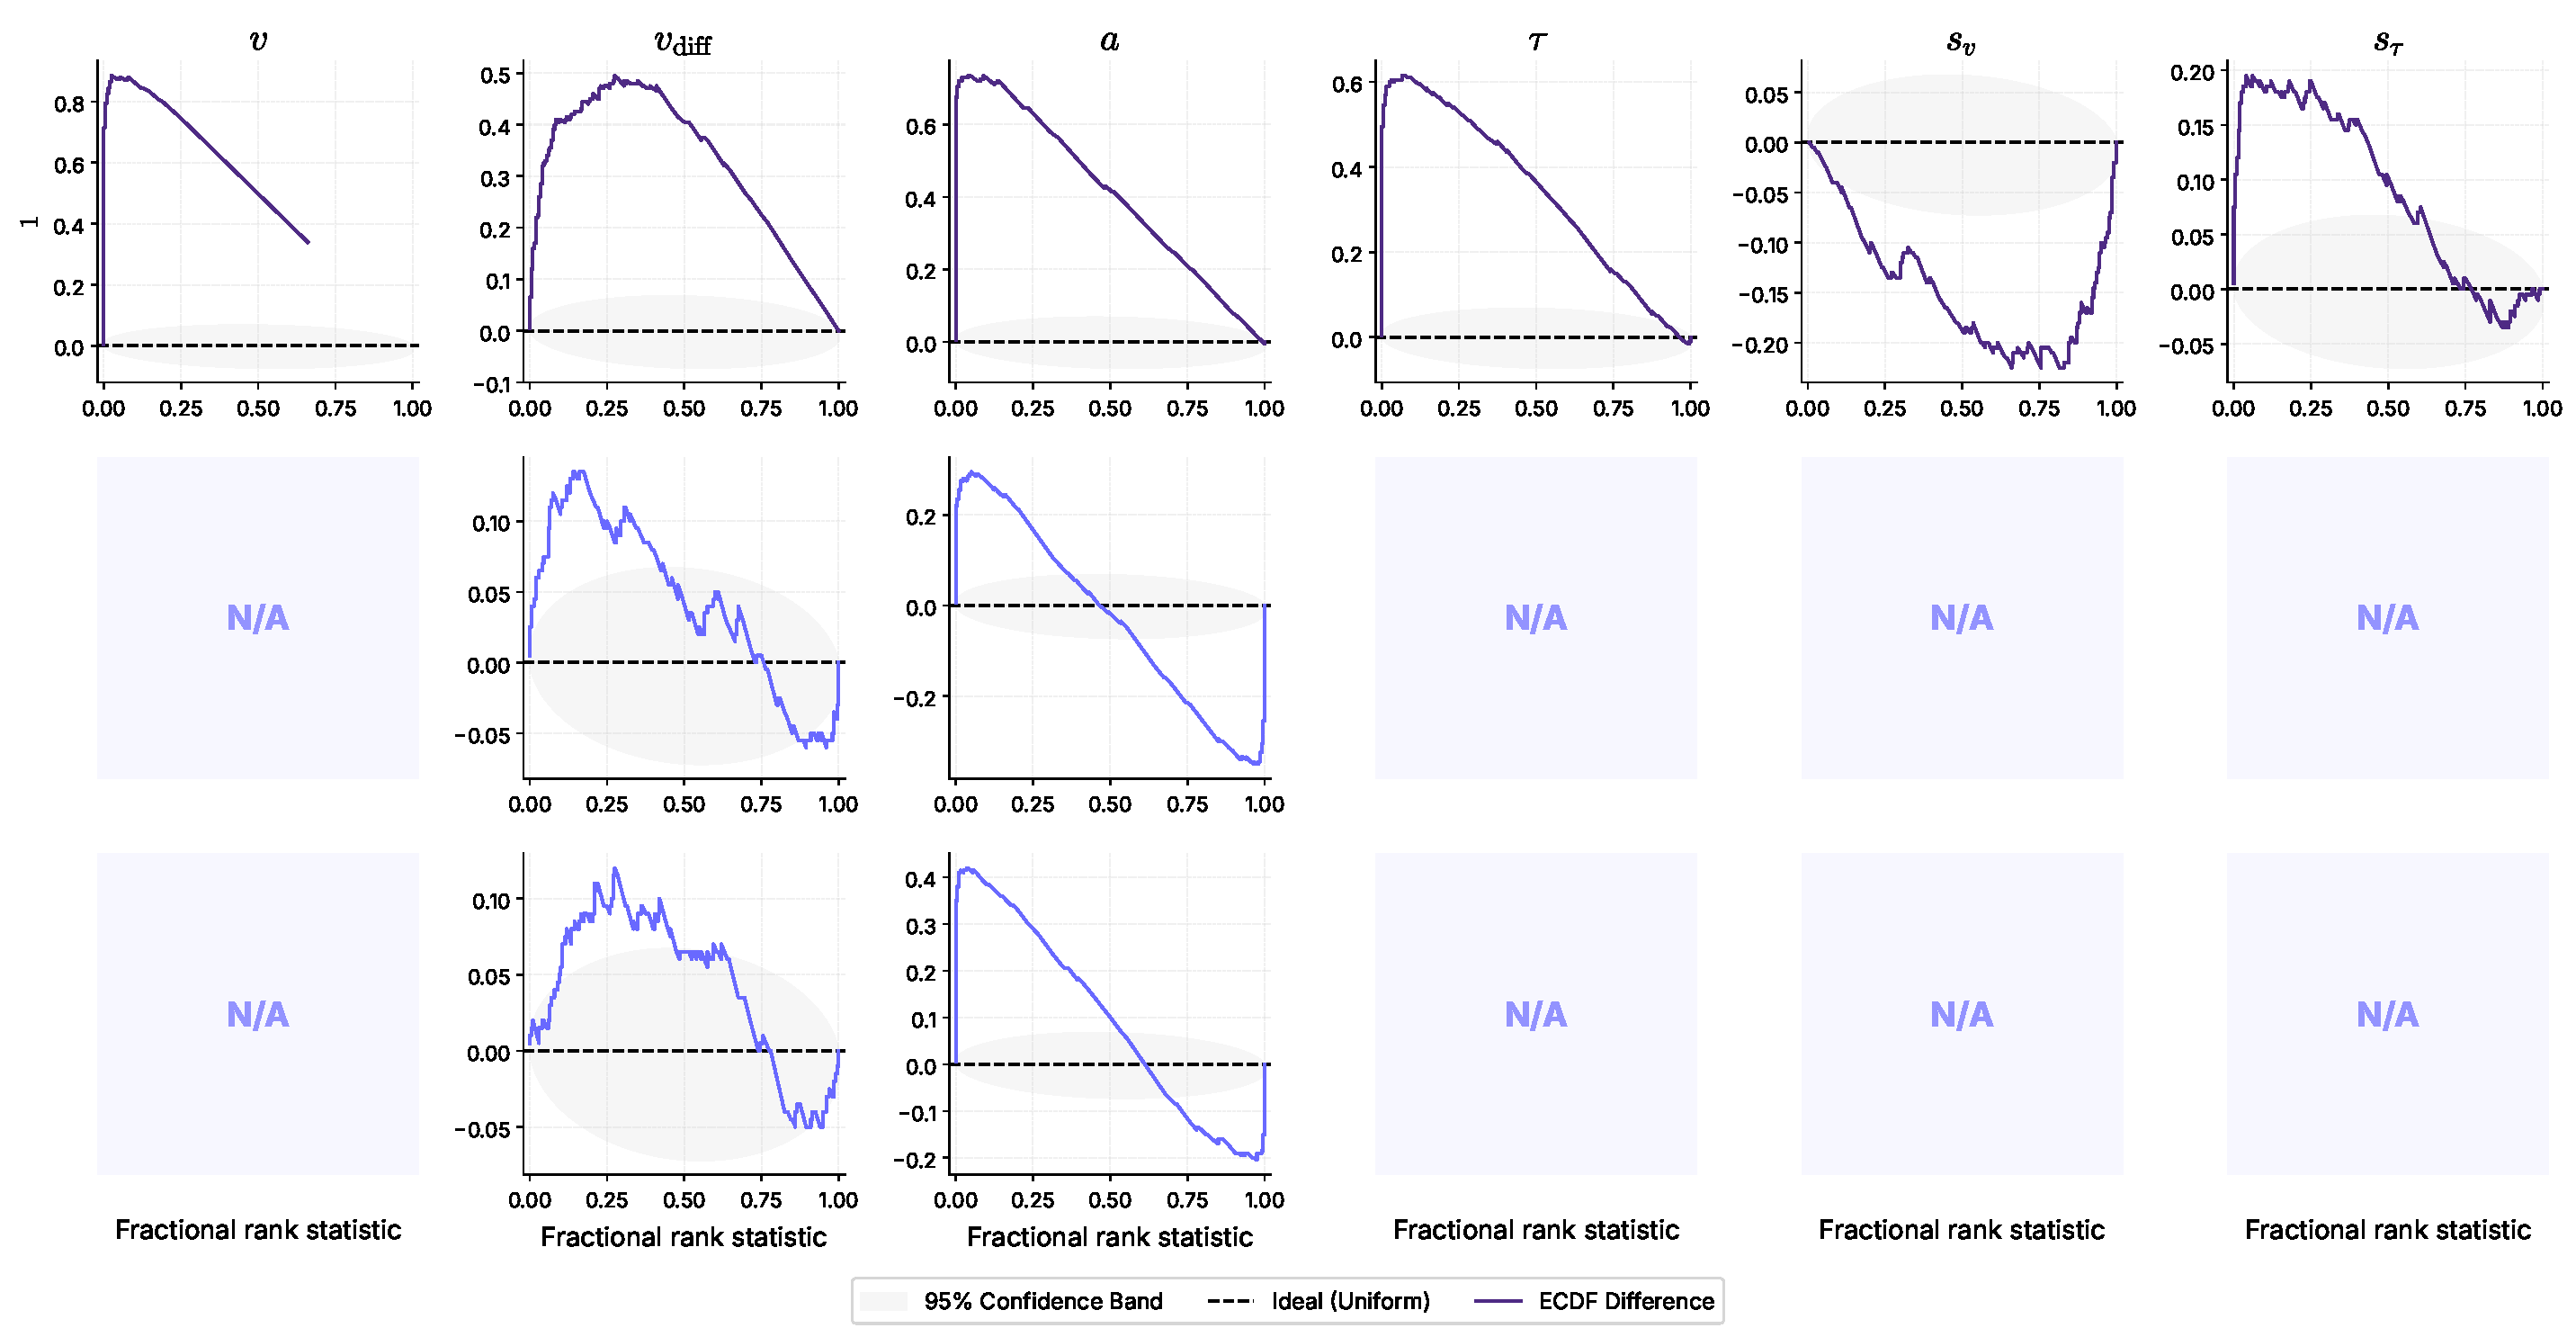
\includegraphics[width=\linewidth,height=0.84\textheight,keepaspectratio]{zeroshot/lba/regressed/ecdf.pdf}
  \caption[LBA, regressed, zero-shot: ECDF calibration]{\textbf{LBA, regressed design, zero-shot --- ECDF calibration.} Rank-ECDF difference (empirical minus uniform) with simultaneous
    95\% confidence bands, on the same cell layout as the corresponding recovery
    figure (Figure~\ref{fig:e3-lba-regressed-zeroshot-rec}). A calibrated posterior stays inside the band;
    excursions above/below indicate bias, and a systematically shallow/steep curve
    indicates over-/under-dispersion.}
  \label{fig:e3-lba-regressed-zeroshot-ecdf}
\end{figure}

\begin{figure}[htbp]
  \centering
  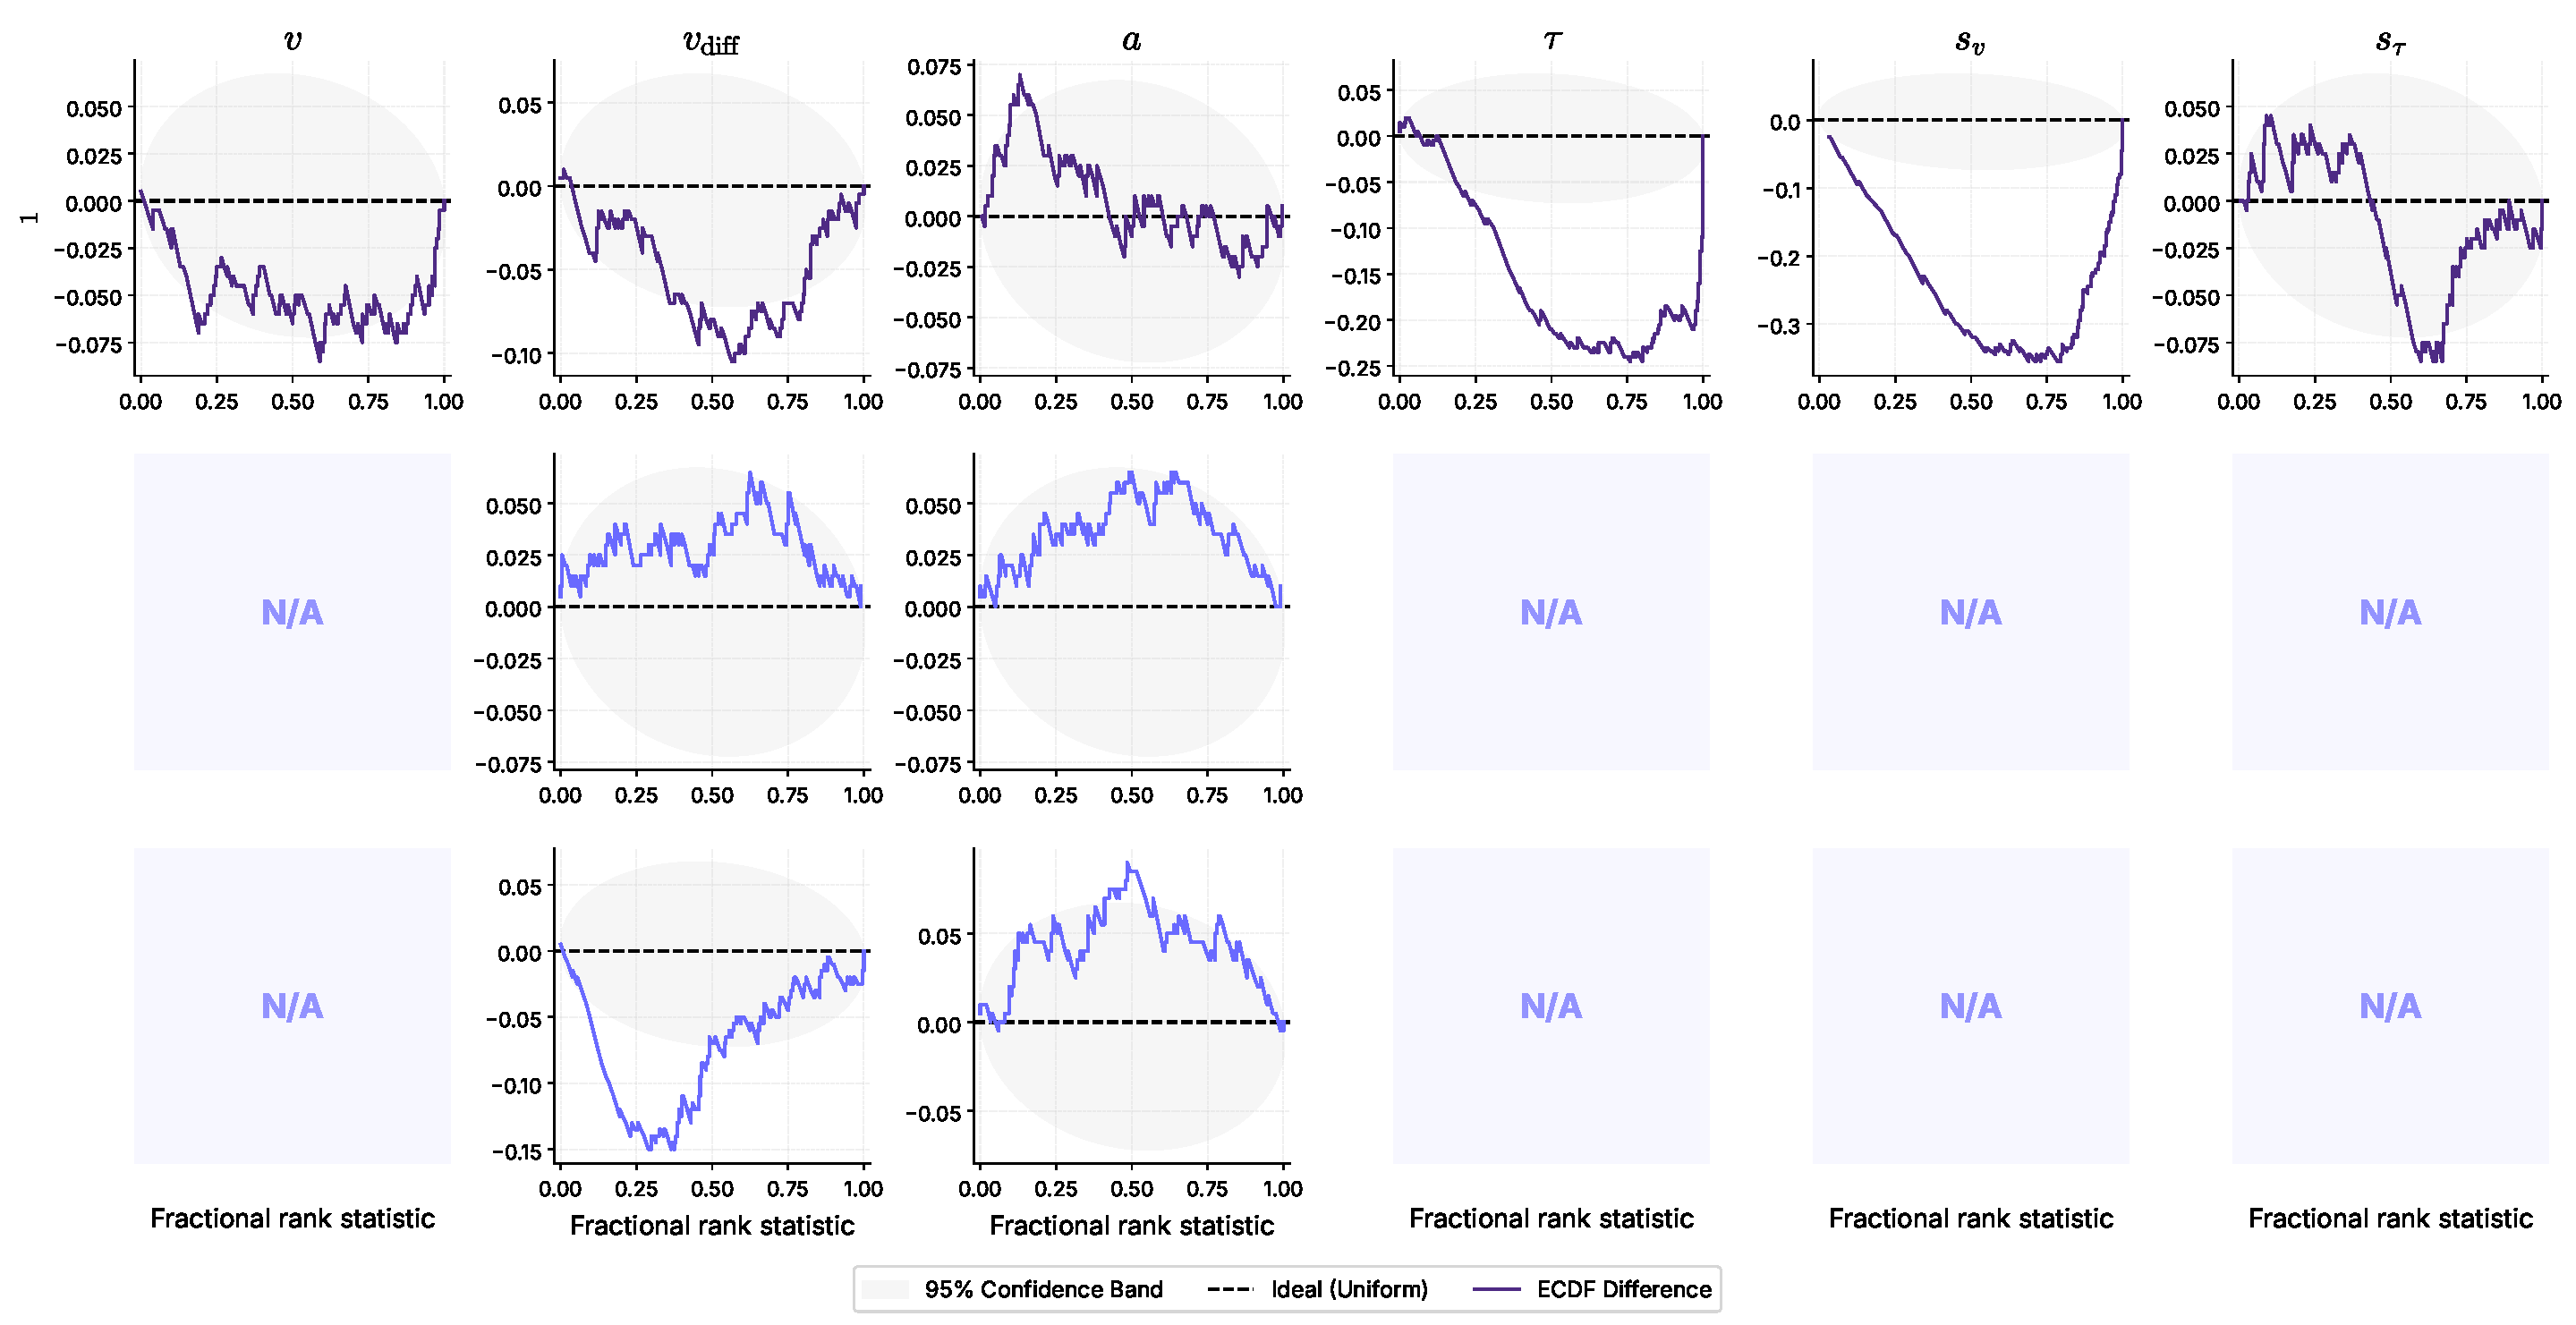
\includegraphics[width=\linewidth,height=0.84\textheight,keepaspectratio]{finetuned/lba/regressed/ecdf.pdf}
  \caption[LBA, regressed, finetuned: ECDF calibration]{\textbf{LBA, regressed design, finetuned --- ECDF calibration.} Rank-ECDF difference (empirical minus uniform) with simultaneous
    95\% confidence bands, on the same cell layout as the corresponding recovery
    figure (Figure~\ref{fig:e3-lba-regressed-finetuned-rec}). A calibrated posterior stays inside the band;
    excursions above/below indicate bias, and a systematically shallow/steep curve
    indicates over-/under-dispersion.}
  \label{fig:e3-lba-regressed-finetuned-ecdf}
\end{figure}

\FloatBarrier
\clearpage

%-----------------------------------------------------------------------------
\subsection{LBA, fixed-regressed design}
\label{sec:e3-lba-fixed_regressed}
%-----------------------------------------------------------------------------

\begin{figure}[htbp]
  \centering
  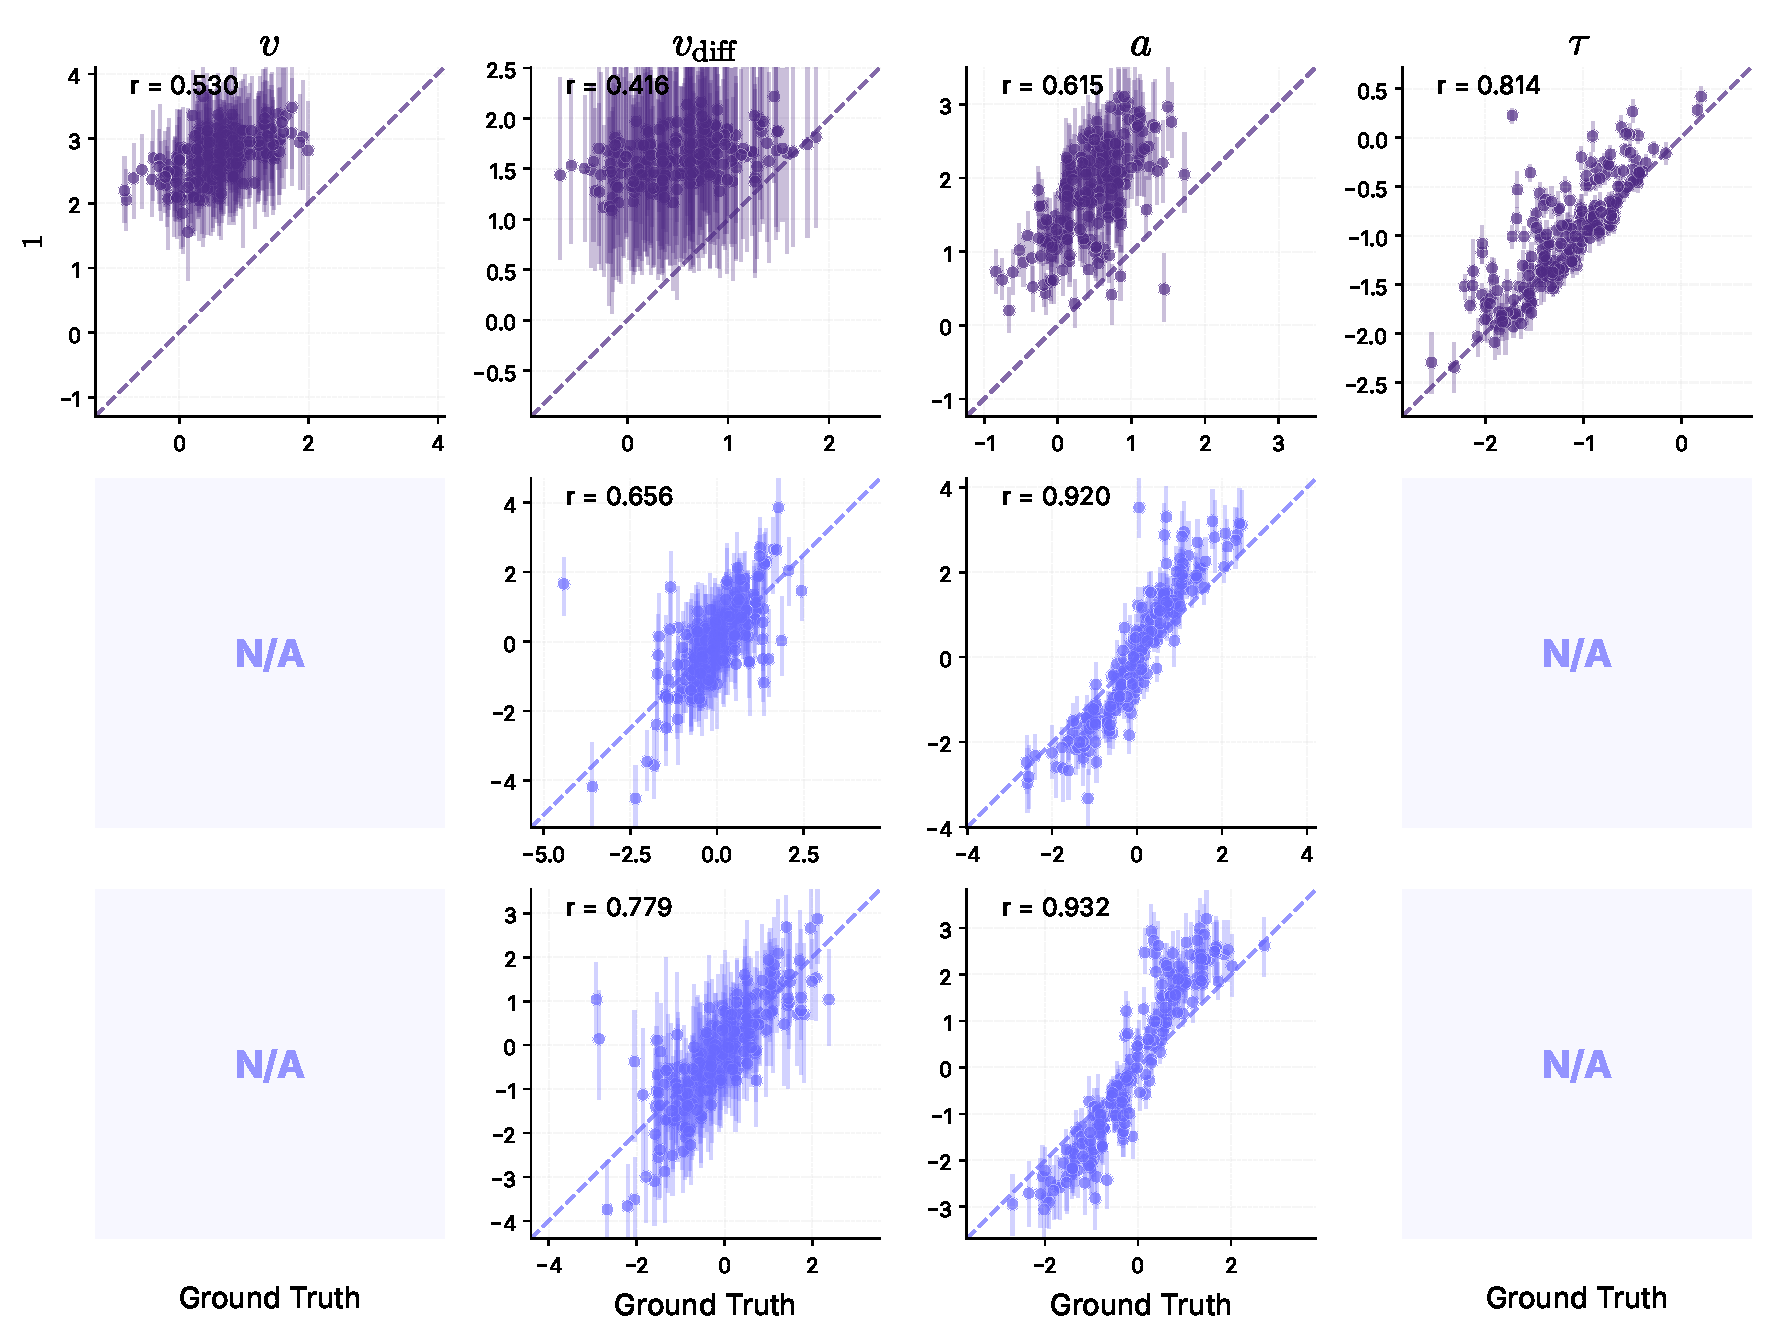
\includegraphics[width=\linewidth,height=0.84\textheight,keepaspectratio]{zeroshot/lba/fixed_regressed/recovery.pdf}
  \caption[LBA, fixed-regressed, zero-shot: recovery]{\textbf{LBA, fixed-regressed design, zero-shot --- coefficient recovery.} Posterior mean (points) with 95\% credible intervals against the
    data-generating value, one panel per active cell of the coefficient matrix
    $\mathbf{B}$. Columns are intrinsic parameters, rows are design columns
    (intercept, main effects, interactions), labeled by regressor and category;
    the panel axes render this as \texttt{predictor|category}. Inactive cells are
    drawn as grey N/A tiles. Point color encodes the row kind: intercept (purple),
    main effect (blue), interaction (red). This arm evaluates the original pre-finetune checkpoint applied to LBA without any LBA training.}
  \label{fig:e3-lba-fixed_regressed-zeroshot-rec}
\end{figure}

\begin{figure}[htbp]
  \centering
  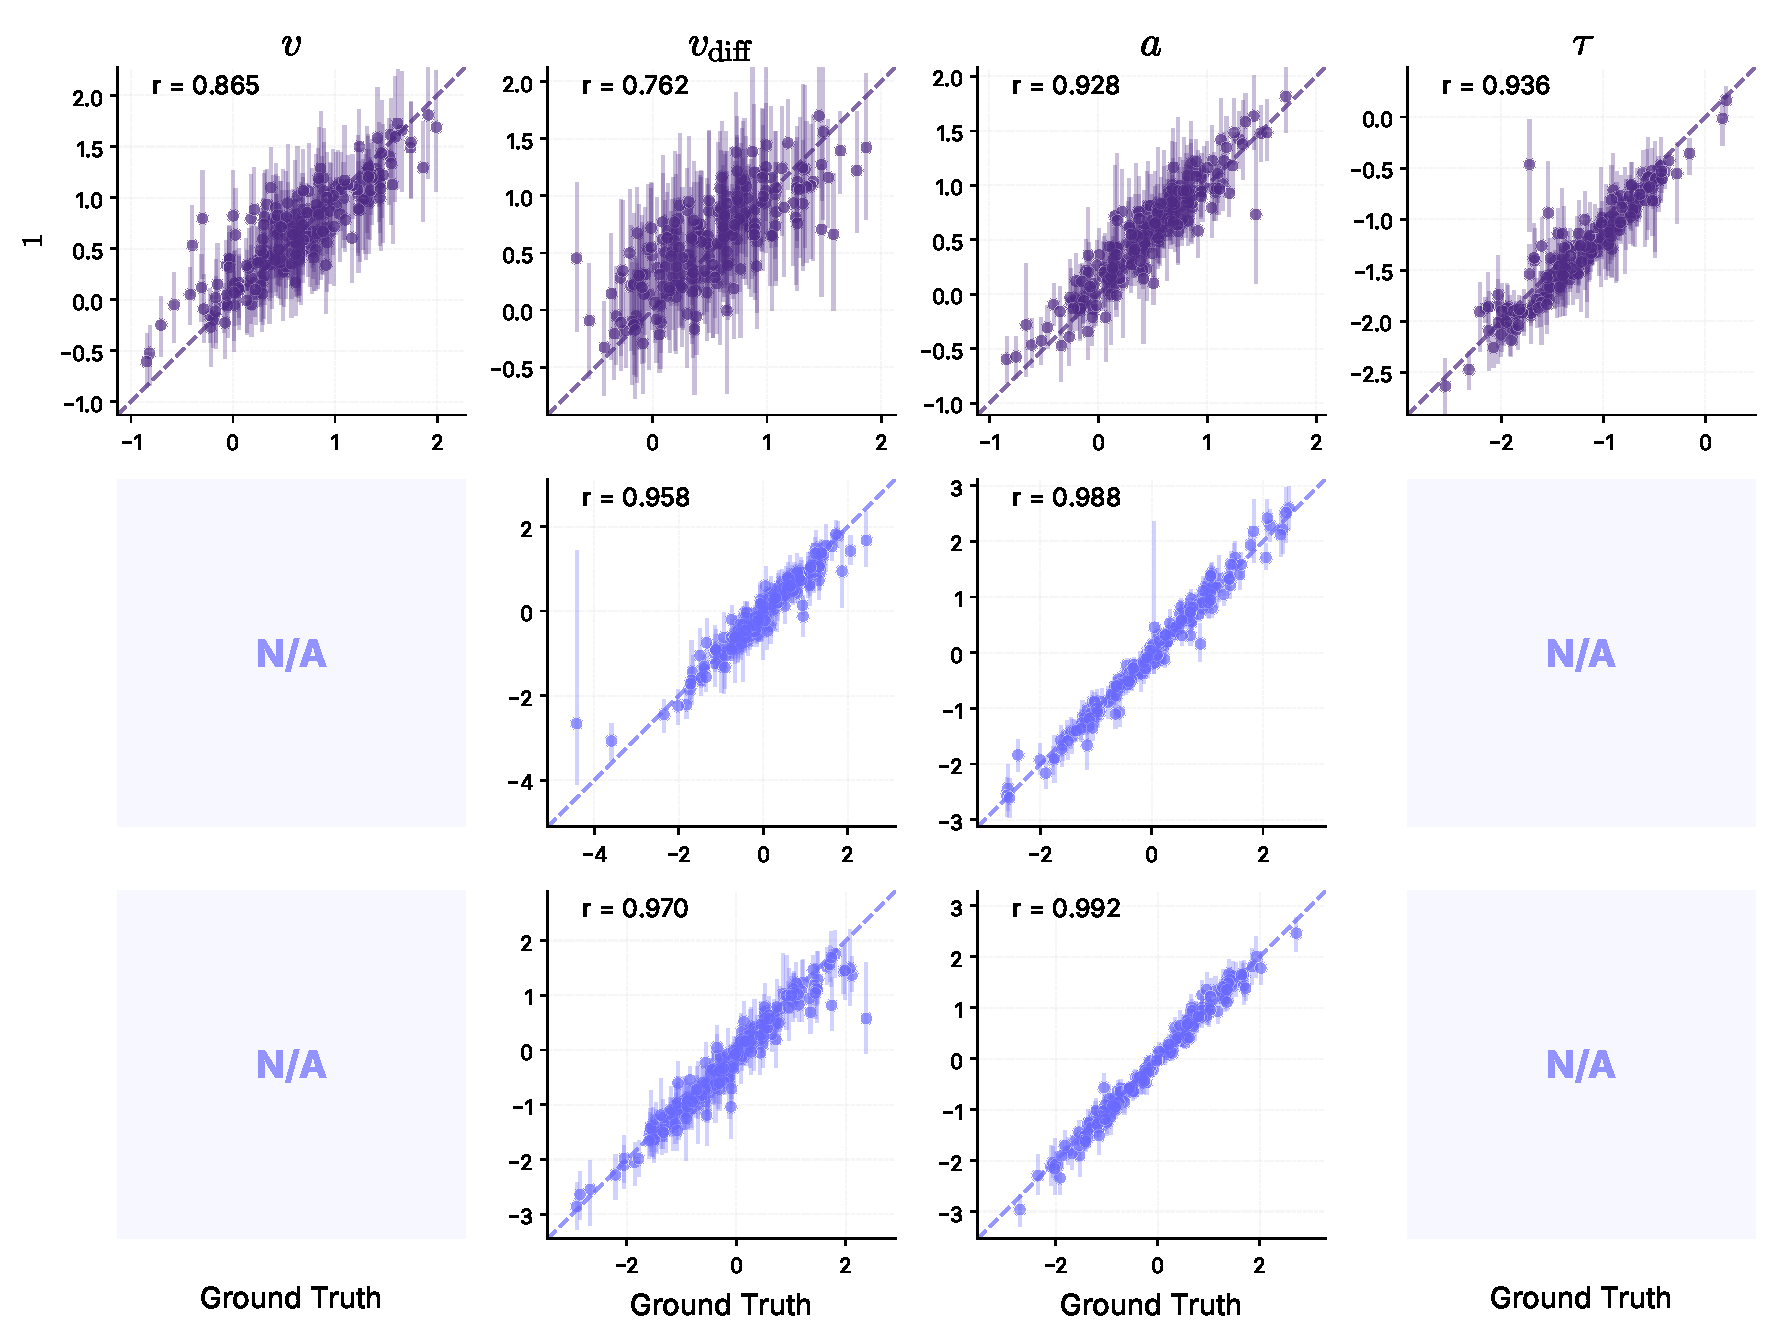
\includegraphics[width=\linewidth,height=0.84\textheight,keepaspectratio]{finetuned/lba/fixed_regressed/recovery.pdf}
  \caption[LBA, fixed-regressed, finetuned: recovery]{\textbf{LBA, fixed-regressed design, finetuned --- coefficient recovery.} Posterior mean (points) with 95\% credible intervals against the
    data-generating value, one panel per active cell of the coefficient matrix
    $\mathbf{B}$. Columns are intrinsic parameters, rows are design columns
    (intercept, main effects, interactions), labeled by regressor and category;
    the panel axes render this as \texttt{predictor|category}. Inactive cells are
    drawn as grey N/A tiles. Point color encodes the row kind: intercept (purple),
    main effect (blue), interaction (red). This arm evaluates the LBA-finetuned checkpoint.}
  \label{fig:e3-lba-fixed_regressed-finetuned-rec}
\end{figure}

\begin{figure}[htbp]
  \centering
  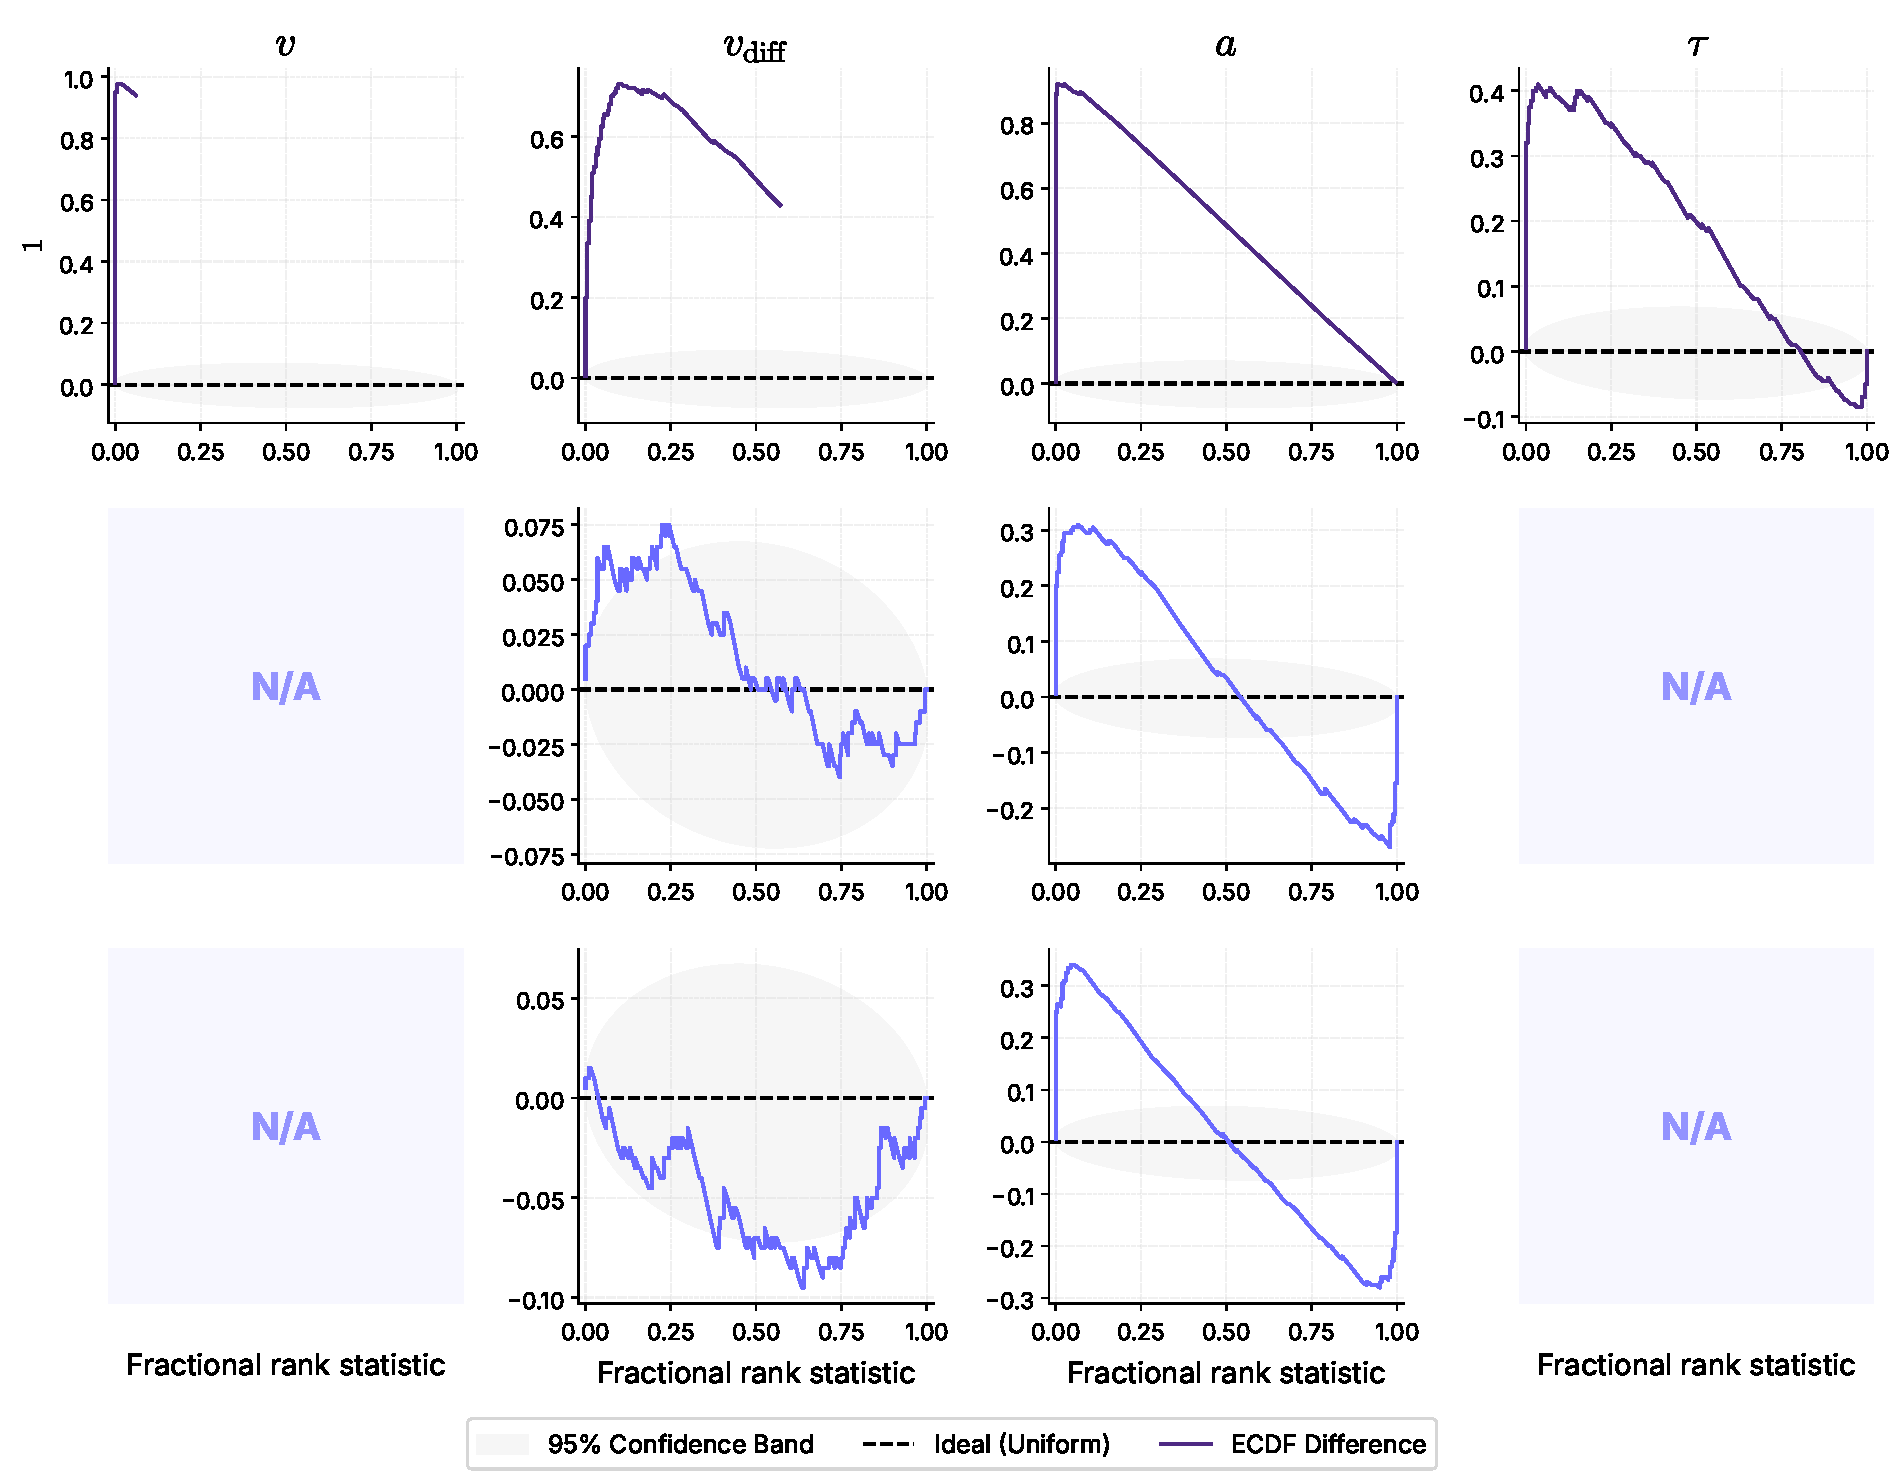
\includegraphics[width=\linewidth,height=0.84\textheight,keepaspectratio]{zeroshot/lba/fixed_regressed/ecdf.pdf}
  \caption[LBA, fixed-regressed, zero-shot: ECDF calibration]{\textbf{LBA, fixed-regressed design, zero-shot --- ECDF calibration.} Rank-ECDF difference (empirical minus uniform) with simultaneous
    95\% confidence bands, on the same cell layout as the corresponding recovery
    figure (Figure~\ref{fig:e3-lba-fixed_regressed-zeroshot-rec}). A calibrated posterior stays inside the band;
    excursions above/below indicate bias, and a systematically shallow/steep curve
    indicates over-/under-dispersion.}
  \label{fig:e3-lba-fixed_regressed-zeroshot-ecdf}
\end{figure}

\begin{figure}[htbp]
  \centering
  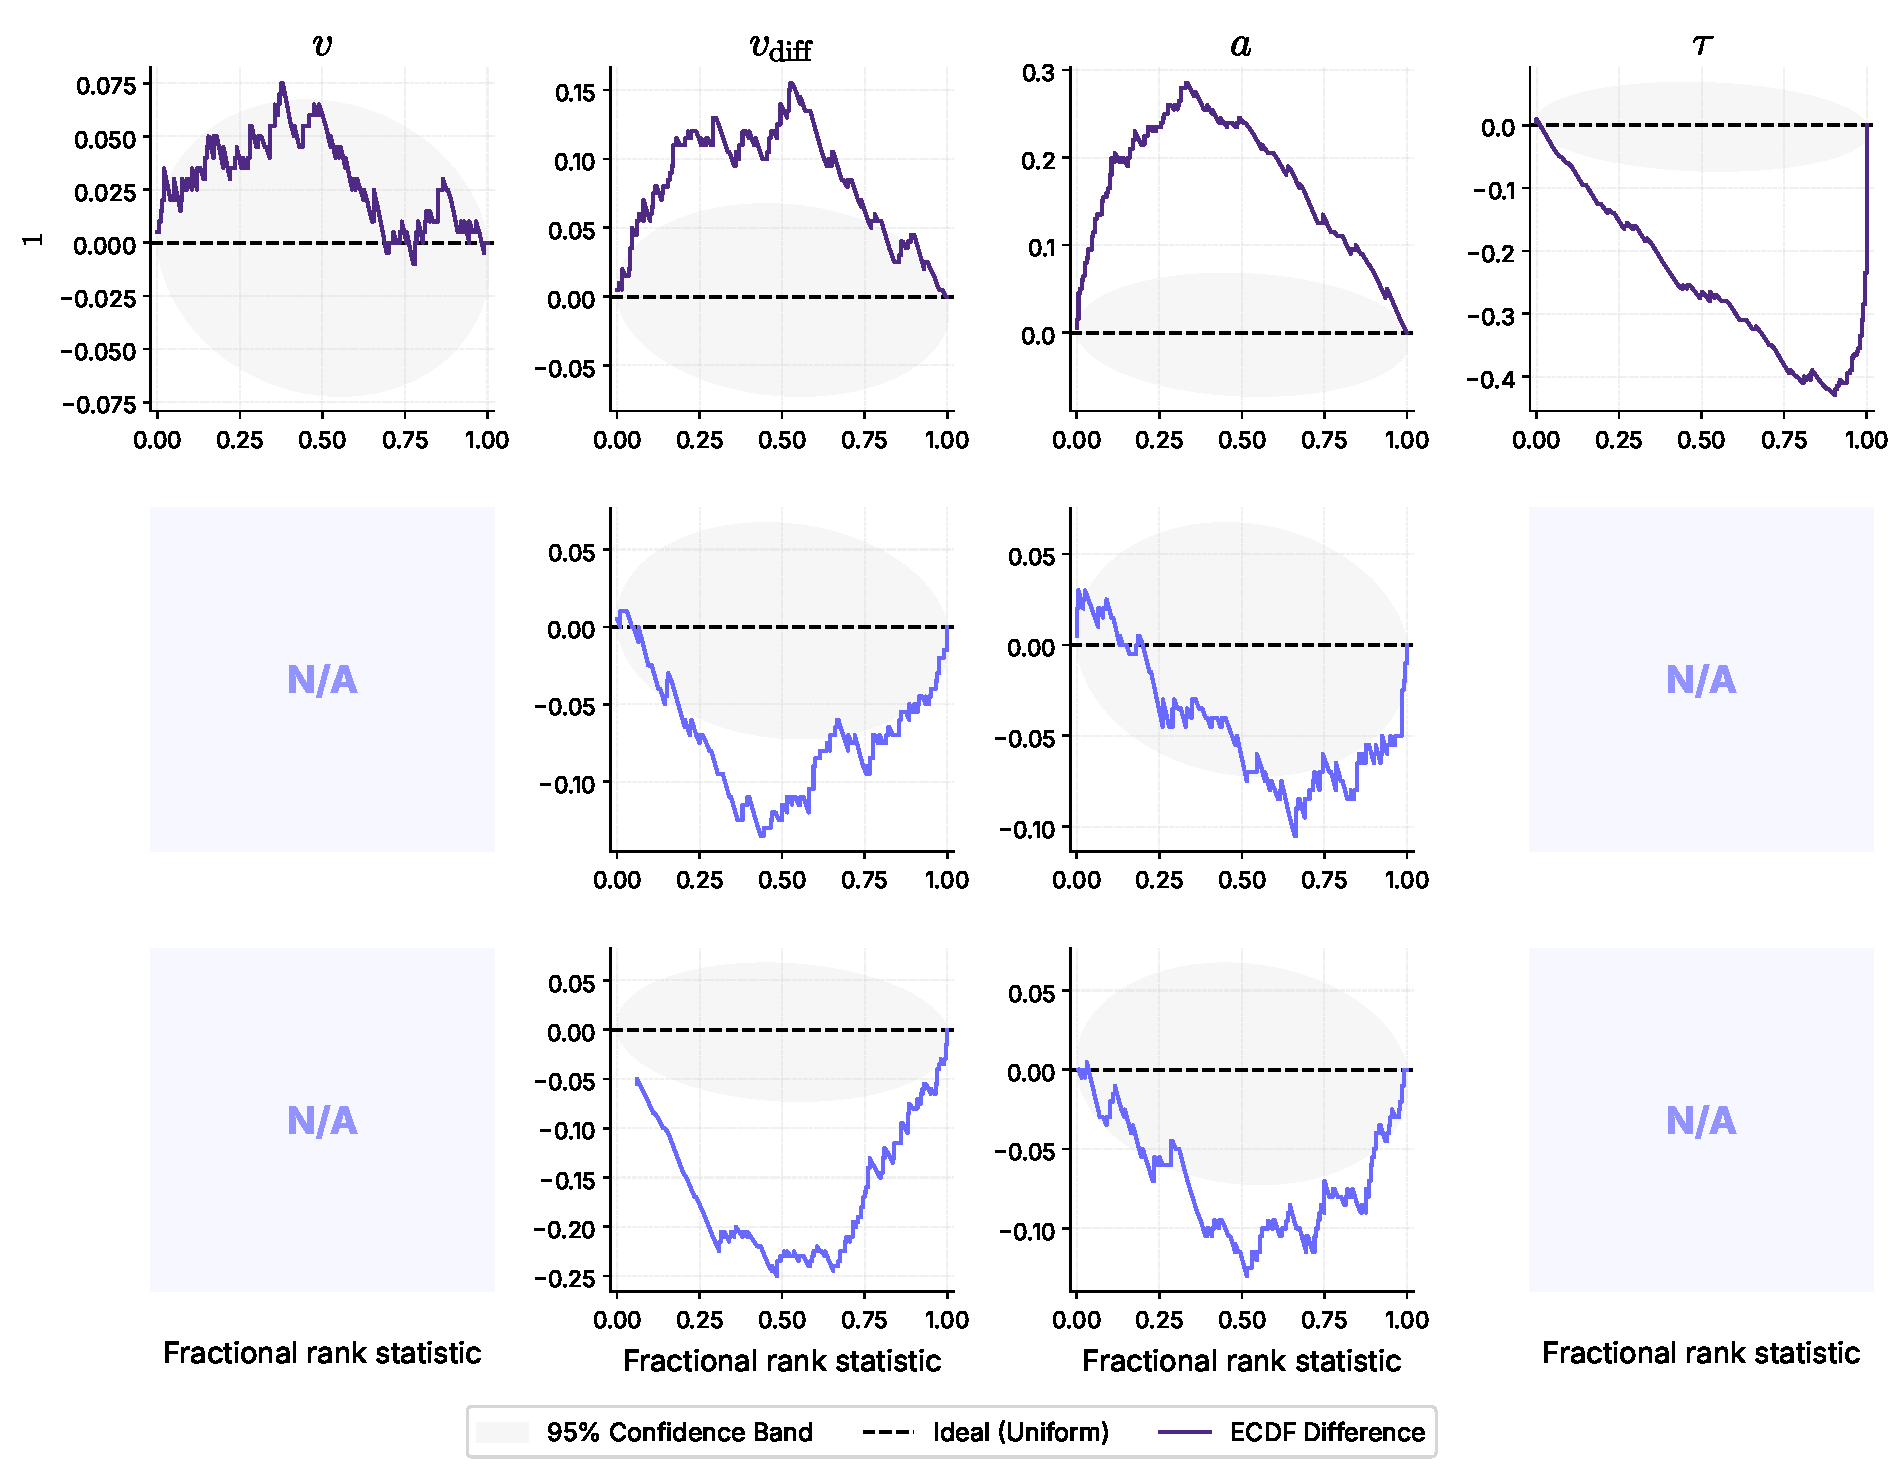
\includegraphics[width=\linewidth,height=0.84\textheight,keepaspectratio]{finetuned/lba/fixed_regressed/ecdf.pdf}
  \caption[LBA, fixed-regressed, finetuned: ECDF calibration]{\textbf{LBA, fixed-regressed design, finetuned --- ECDF calibration.} Rank-ECDF difference (empirical minus uniform) with simultaneous
    95\% confidence bands, on the same cell layout as the corresponding recovery
    figure (Figure~\ref{fig:e3-lba-fixed_regressed-finetuned-rec}). A calibrated posterior stays inside the band;
    excursions above/below indicate bias, and a systematically shallow/steep curve
    indicates over-/under-dispersion.}
  \label{fig:e3-lba-fixed_regressed-finetuned-ecdf}
\end{figure}

\FloatBarrier
\clearpage

%-----------------------------------------------------------------------------
\subsection{LBA, interaction design}
\label{sec:e3-lba-interaction}
%-----------------------------------------------------------------------------

\begin{figure}[htbp]
  \centering
  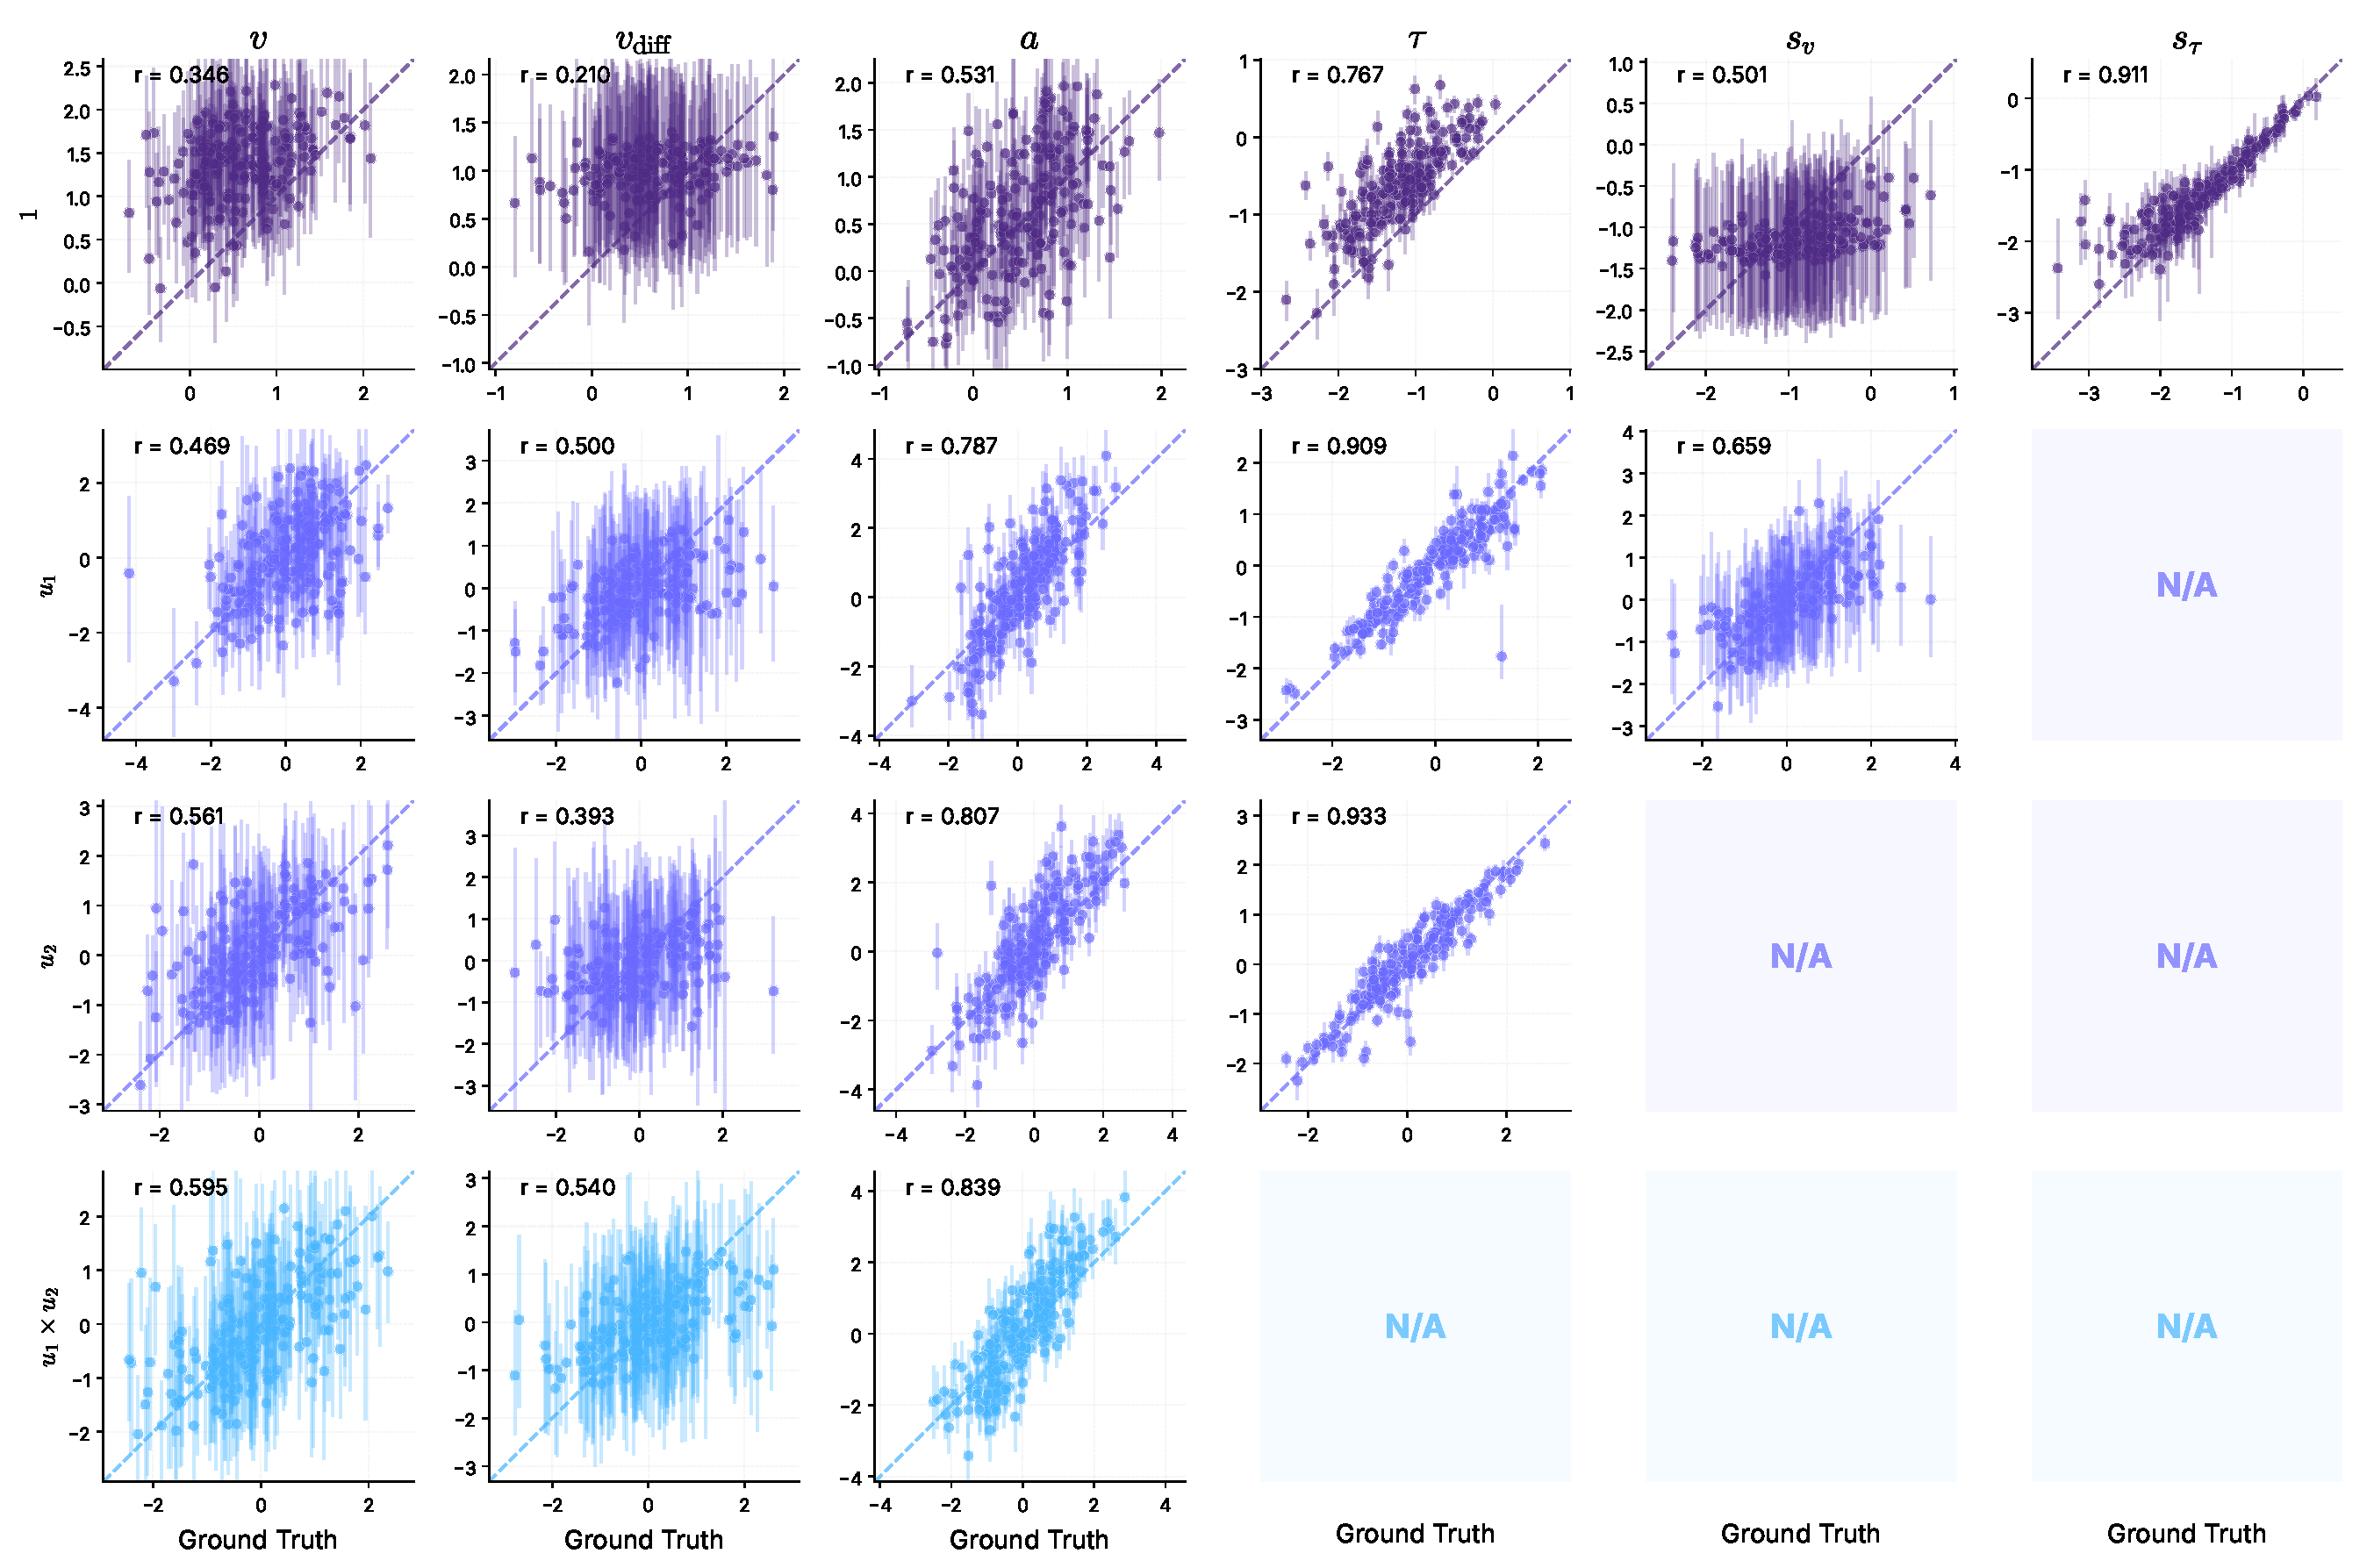
\includegraphics[width=\linewidth,height=0.84\textheight,keepaspectratio]{zeroshot/lba/interaction/recovery.pdf}
  \caption[LBA, interaction, zero-shot: recovery]{\textbf{LBA, interaction design, zero-shot --- coefficient recovery.} Posterior mean (points) with 95\% credible intervals against the
    data-generating value, one panel per active cell of the coefficient matrix
    $\mathbf{B}$. Columns are intrinsic parameters, rows are design columns
    (intercept, main effects, interactions), labeled by regressor and category;
    the panel axes render this as \texttt{predictor|category}. Inactive cells are
    drawn as grey N/A tiles. Point color encodes the row kind: intercept (purple),
    main effect (blue), interaction (red). This arm evaluates the original pre-finetune checkpoint applied to LBA without any LBA training.}
  \label{fig:e3-lba-interaction-zeroshot-rec}
\end{figure}

\begin{figure}[htbp]
  \centering
  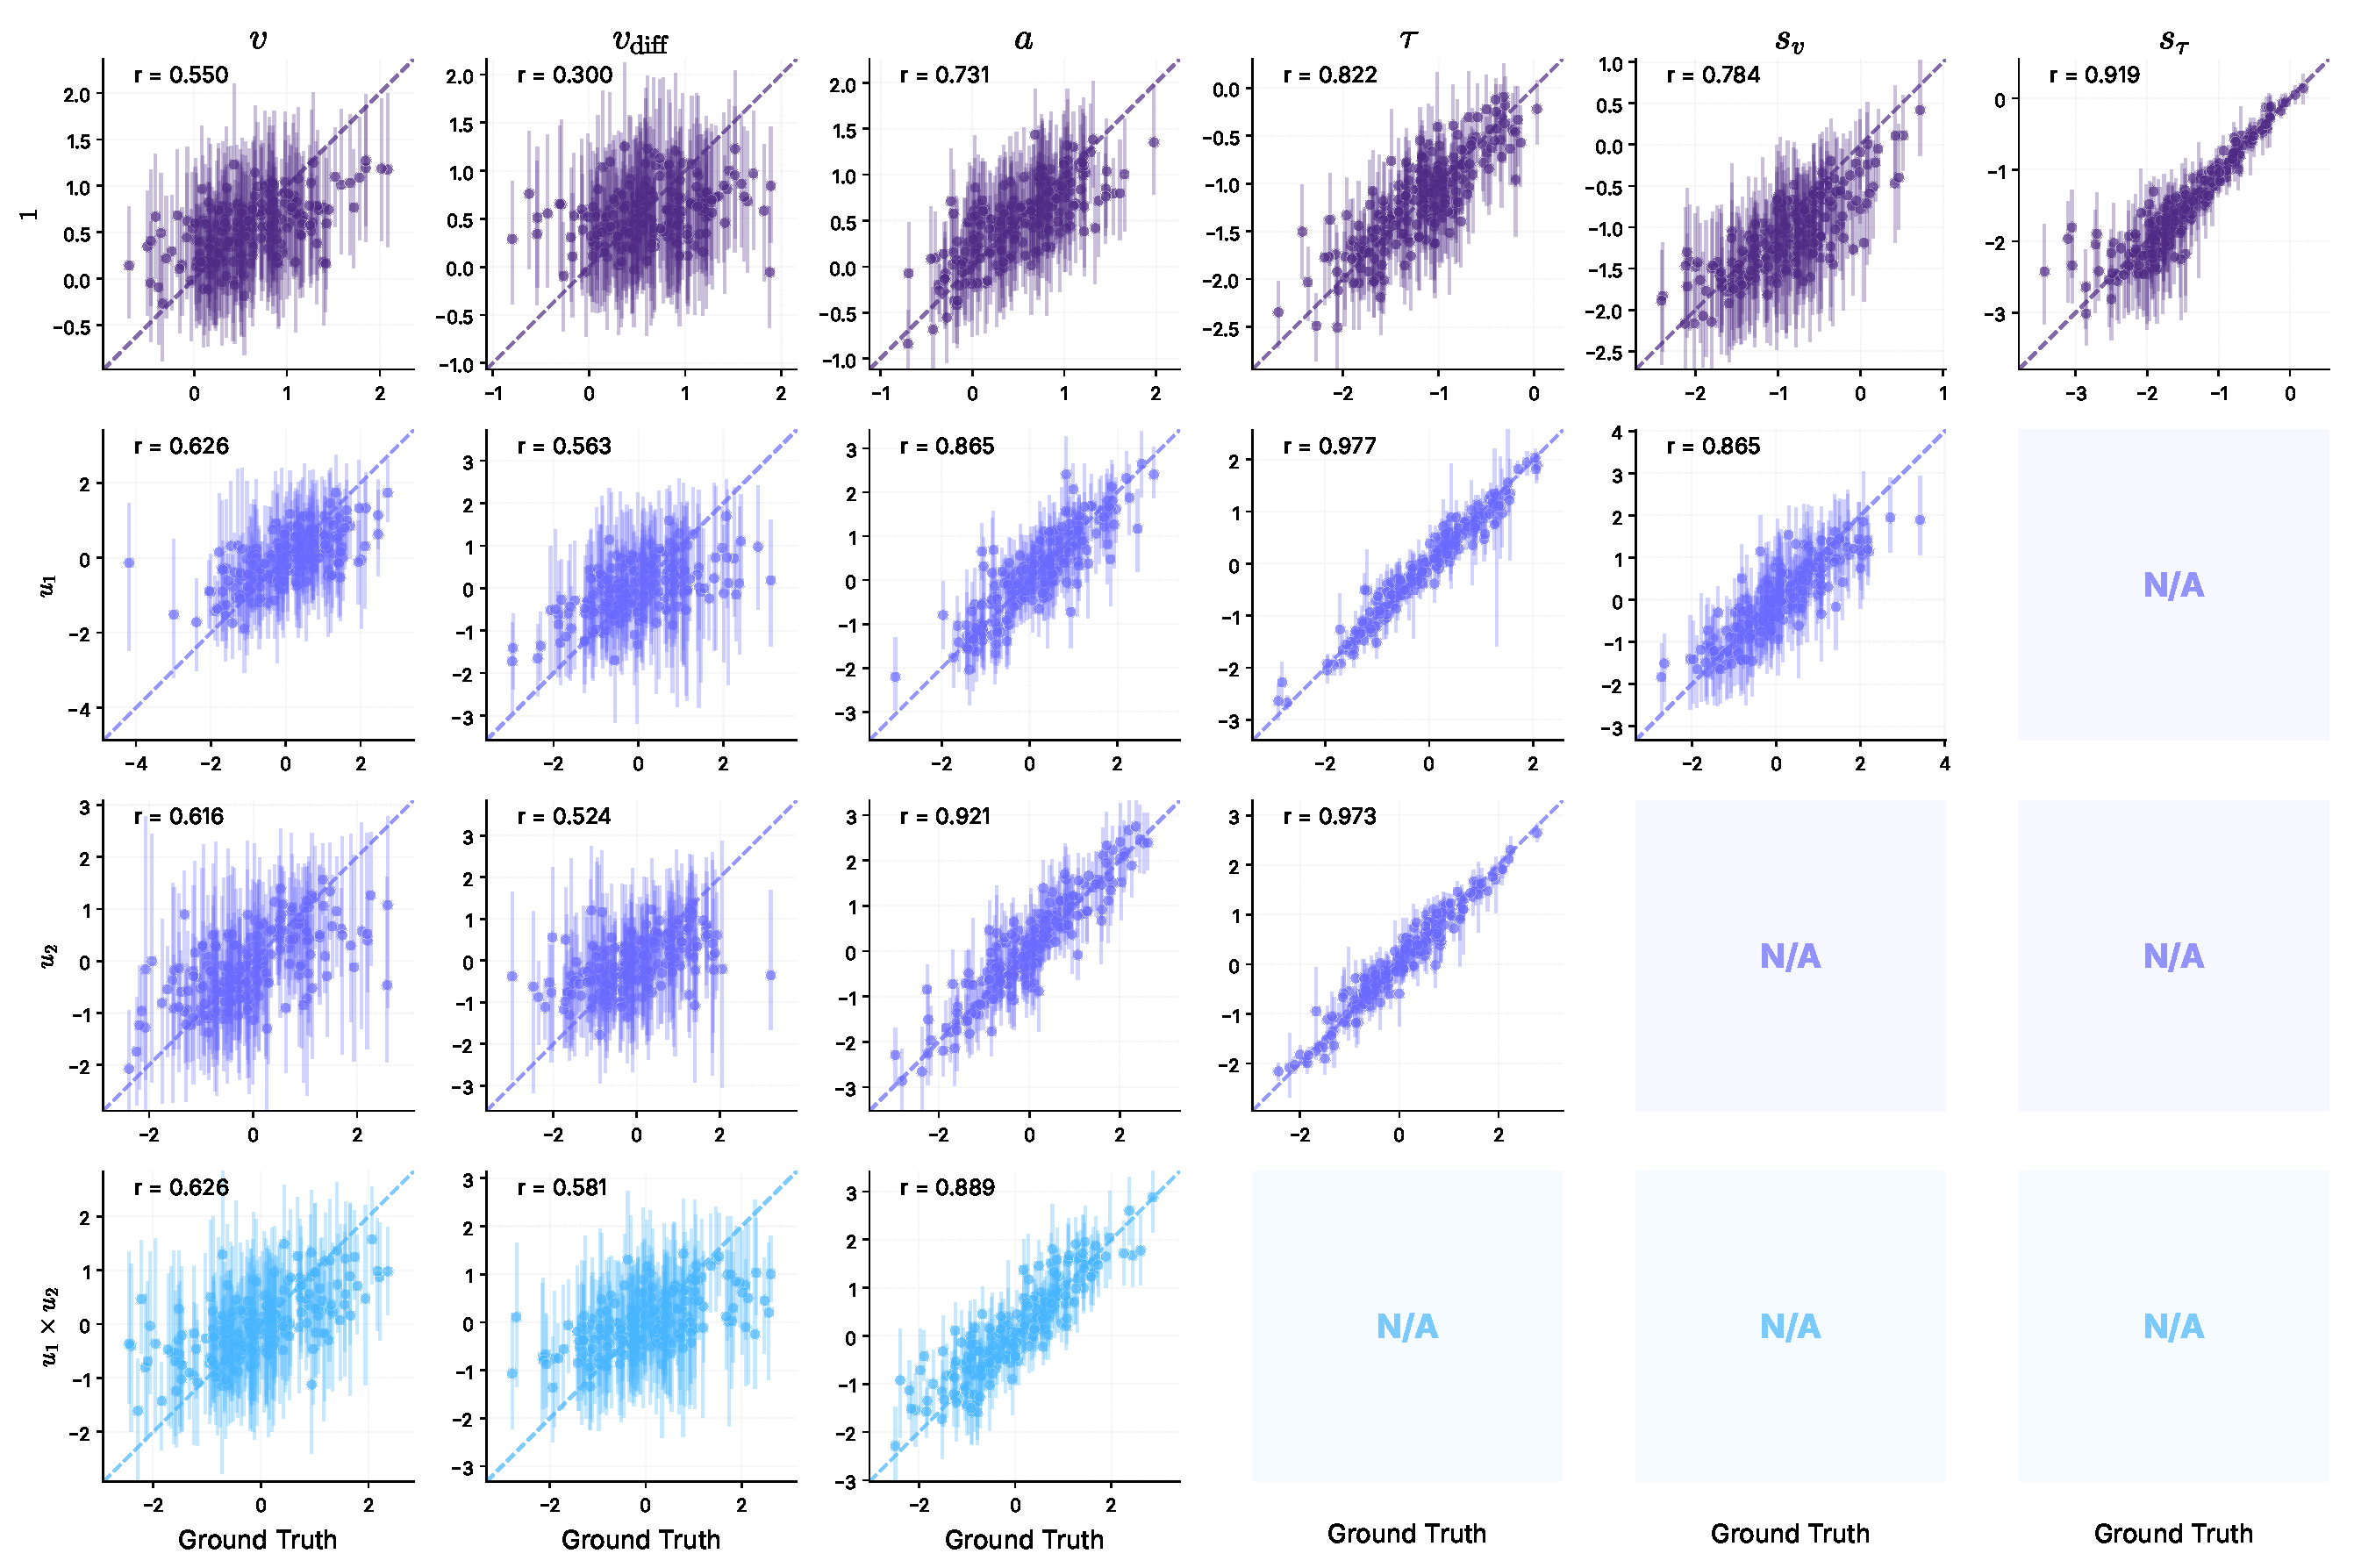
\includegraphics[width=\linewidth,height=0.84\textheight,keepaspectratio]{finetuned/lba/interaction/recovery.pdf}
  \caption[LBA, interaction, finetuned: recovery]{\textbf{LBA, interaction design, finetuned --- coefficient recovery.} Posterior mean (points) with 95\% credible intervals against the
    data-generating value, one panel per active cell of the coefficient matrix
    $\mathbf{B}$. Columns are intrinsic parameters, rows are design columns
    (intercept, main effects, interactions), labeled by regressor and category;
    the panel axes render this as \texttt{predictor|category}. Inactive cells are
    drawn as grey N/A tiles. Point color encodes the row kind: intercept (purple),
    main effect (blue), interaction (red). This arm evaluates the LBA-finetuned checkpoint.}
  \label{fig:e3-lba-interaction-finetuned-rec}
\end{figure}

\begin{figure}[htbp]
  \centering
  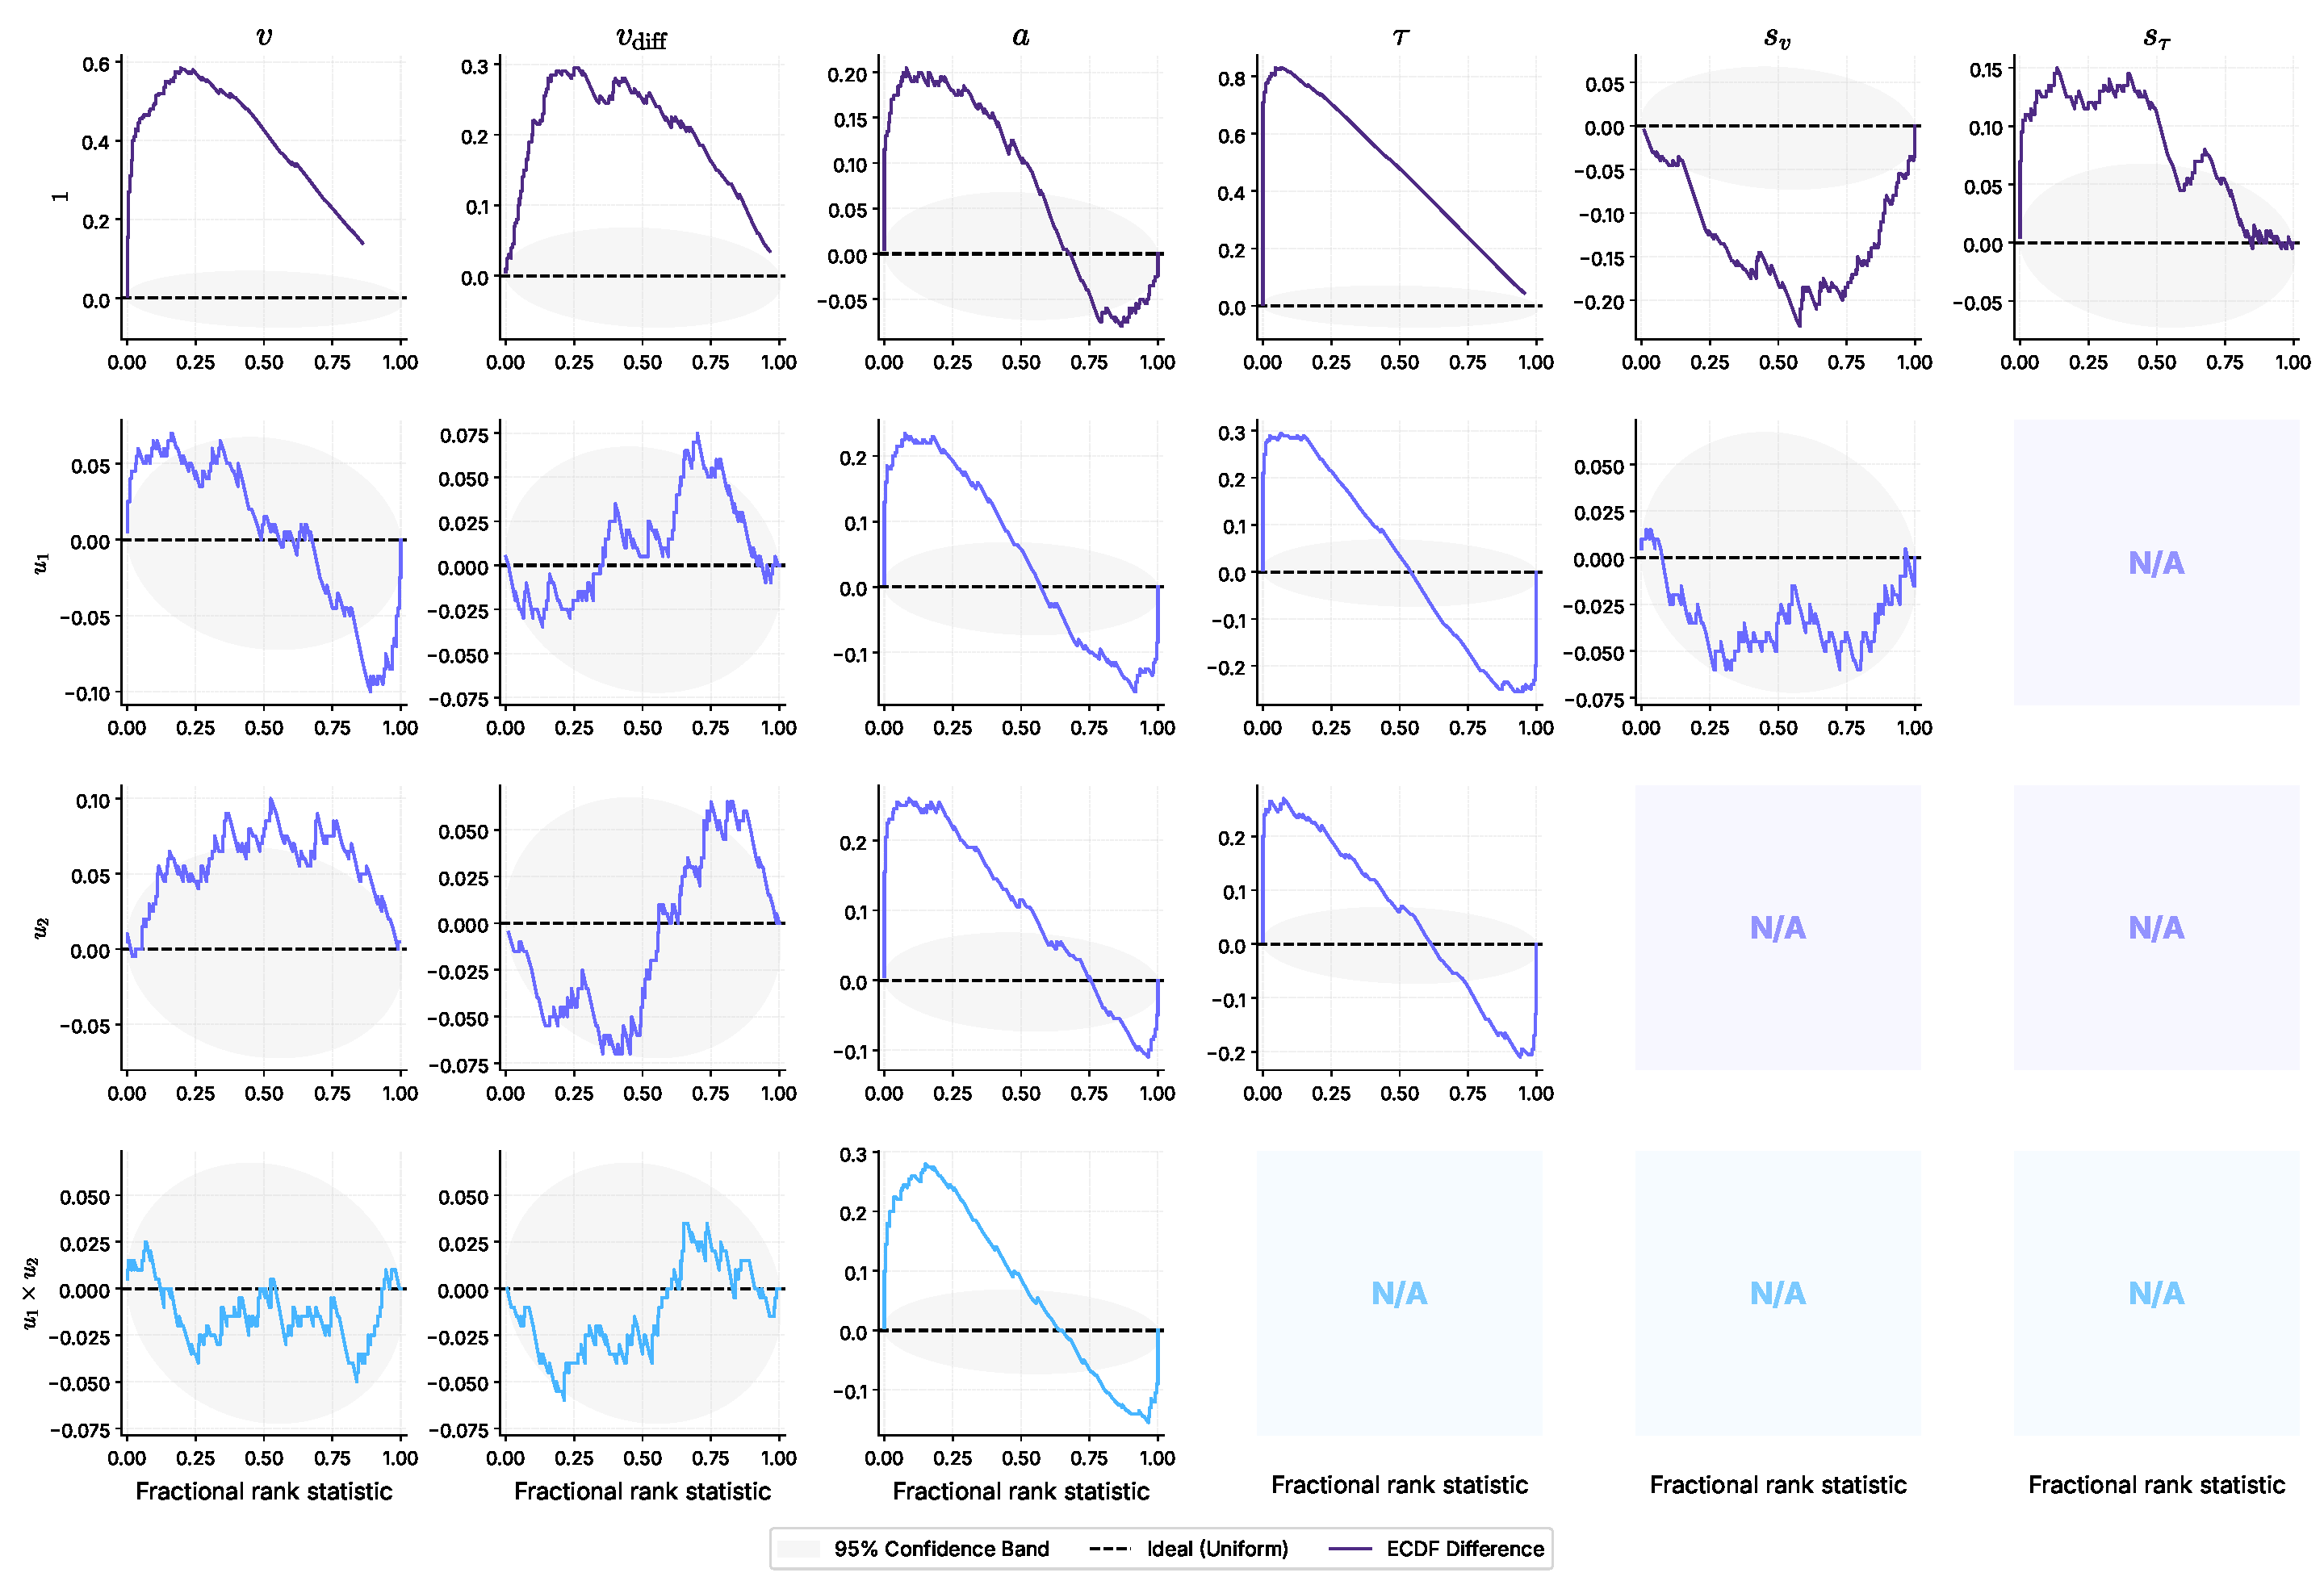
\includegraphics[width=\linewidth,height=0.84\textheight,keepaspectratio]{zeroshot/lba/interaction/ecdf.pdf}
  \caption[LBA, interaction, zero-shot: ECDF calibration]{\textbf{LBA, interaction design, zero-shot --- ECDF calibration.} Rank-ECDF difference (empirical minus uniform) with simultaneous
    95\% confidence bands, on the same cell layout as the corresponding recovery
    figure (Figure~\ref{fig:e3-lba-interaction-zeroshot-rec}). A calibrated posterior stays inside the band;
    excursions above/below indicate bias, and a systematically shallow/steep curve
    indicates over-/under-dispersion.}
  \label{fig:e3-lba-interaction-zeroshot-ecdf}
\end{figure}

\begin{figure}[htbp]
  \centering
  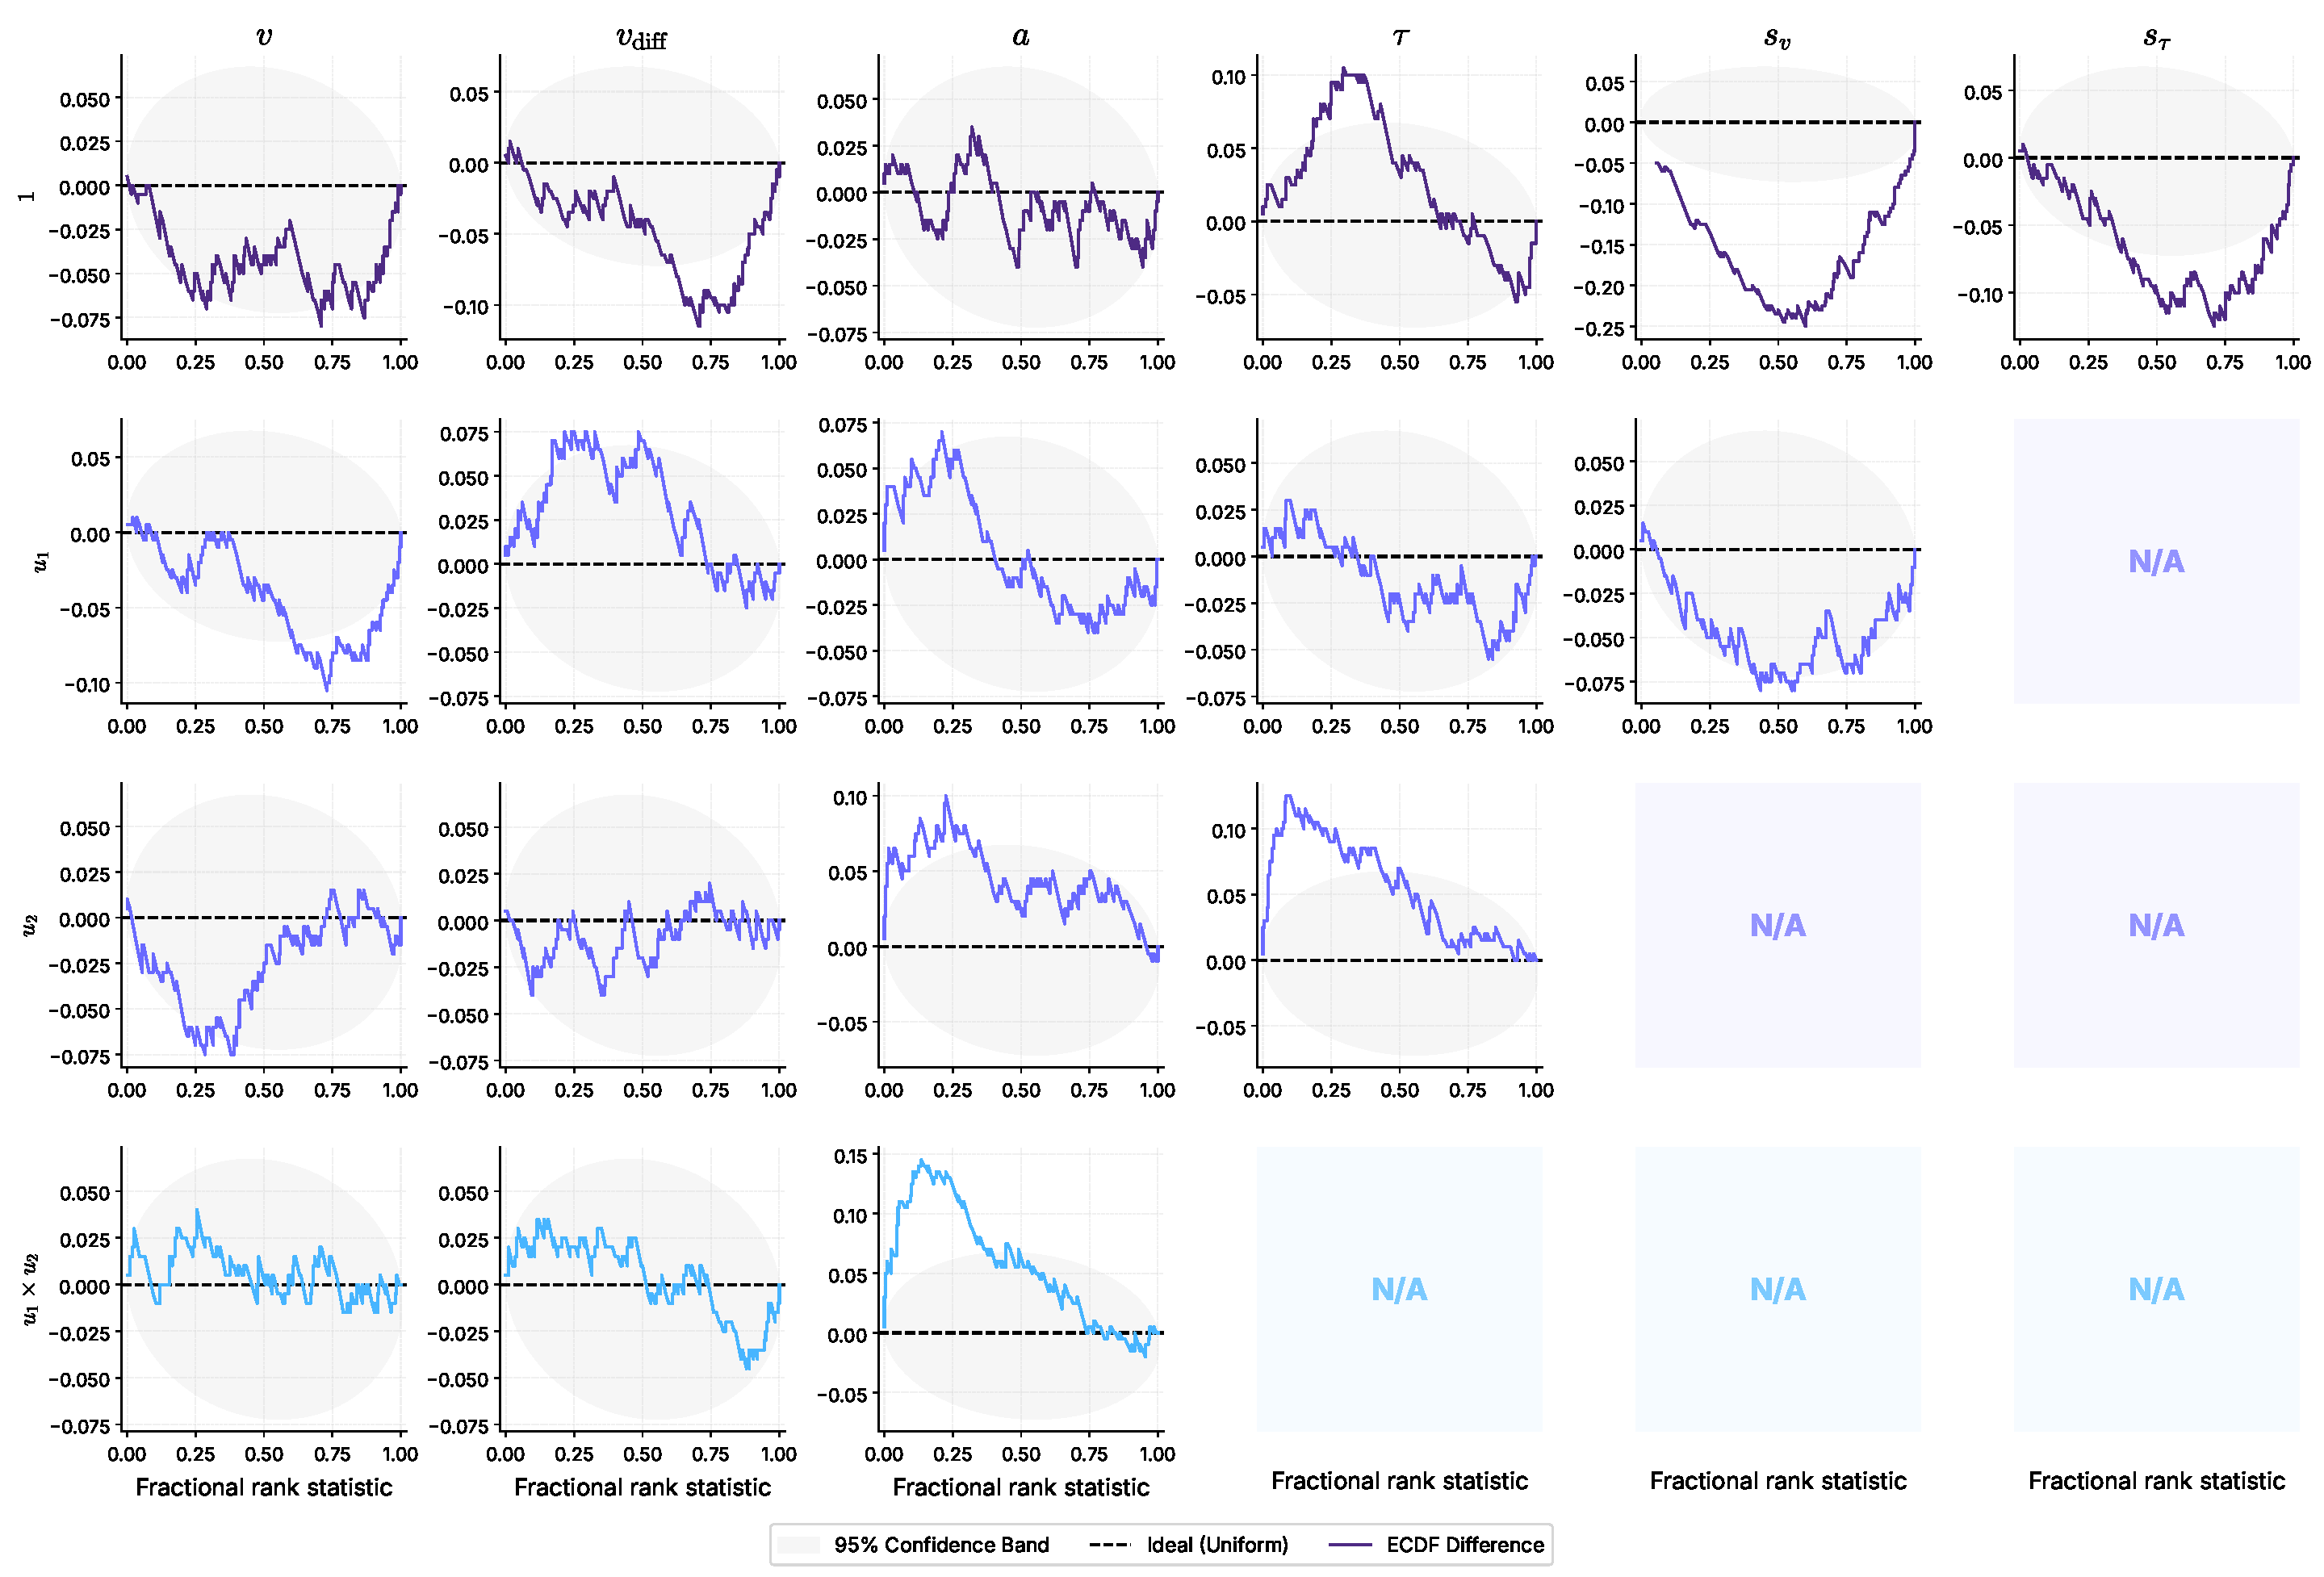
\includegraphics[width=\linewidth,height=0.84\textheight,keepaspectratio]{finetuned/lba/interaction/ecdf.pdf}
  \caption[LBA, interaction, finetuned: ECDF calibration]{\textbf{LBA, interaction design, finetuned --- ECDF calibration.} Rank-ECDF difference (empirical minus uniform) with simultaneous
    95\% confidence bands, on the same cell layout as the corresponding recovery
    figure (Figure~\ref{fig:e3-lba-interaction-finetuned-rec}). A calibrated posterior stays inside the band;
    excursions above/below indicate bias, and a systematically shallow/steep curve
    indicates over-/under-dispersion.}
  \label{fig:e3-lba-interaction-finetuned-ecdf}
\end{figure}

\FloatBarrier
\clearpage

%-----------------------------------------------------------------------------
\subsection{LBA, fixed design}
\label{sec:e3-lba-fixed}
%-----------------------------------------------------------------------------

\begin{figure}[htbp]
  \centering
  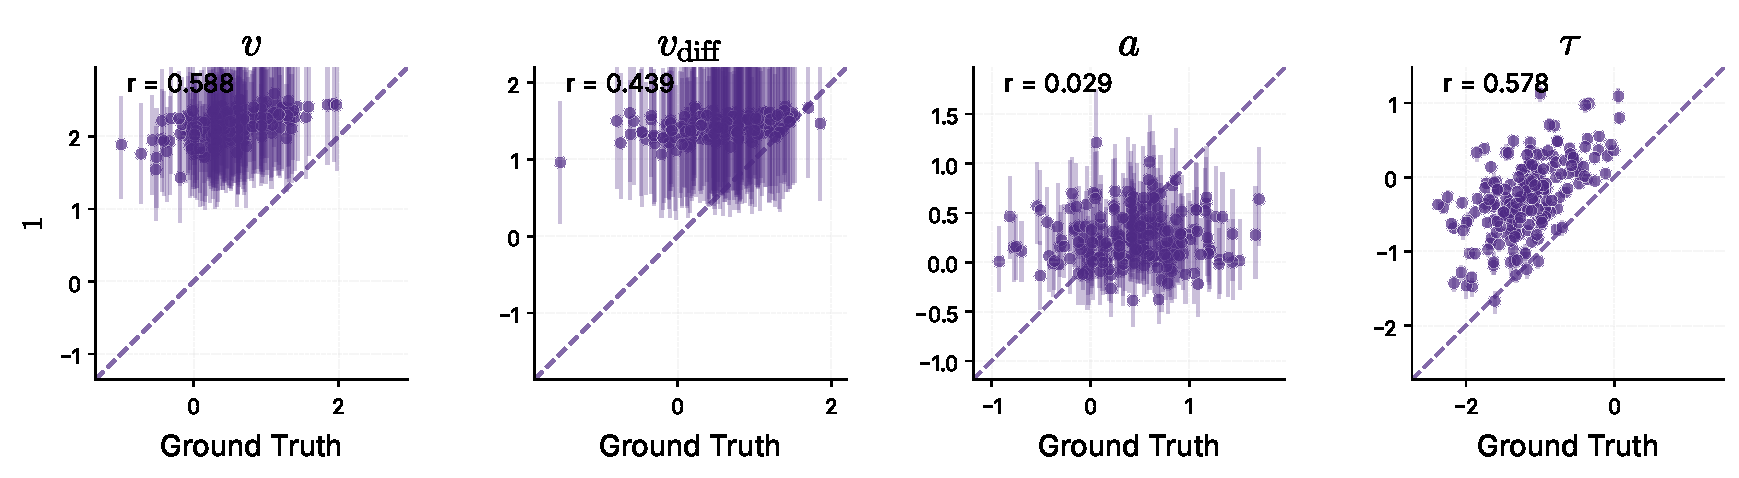
\includegraphics[width=\linewidth,height=0.84\textheight,keepaspectratio]{zeroshot/lba/fixed/recovery.pdf}
  \caption[LBA, fixed, zero-shot: recovery]{\textbf{LBA, fixed design, zero-shot --- coefficient recovery.} Posterior mean (points) with 95\% credible intervals against the
    data-generating value, one panel per active cell of the coefficient matrix
    $\mathbf{B}$. Columns are intrinsic parameters, rows are design columns
    (intercept, main effects, interactions), labeled by regressor and category;
    the panel axes render this as \texttt{predictor|category}. Inactive cells are
    drawn as grey N/A tiles. Point color encodes the row kind: intercept (purple),
    main effect (blue), interaction (red). This arm evaluates the original pre-finetune checkpoint applied to LBA without any LBA training.}
  \label{fig:e3-lba-fixed-zeroshot-rec}
\end{figure}

\begin{figure}[htbp]
  \centering
  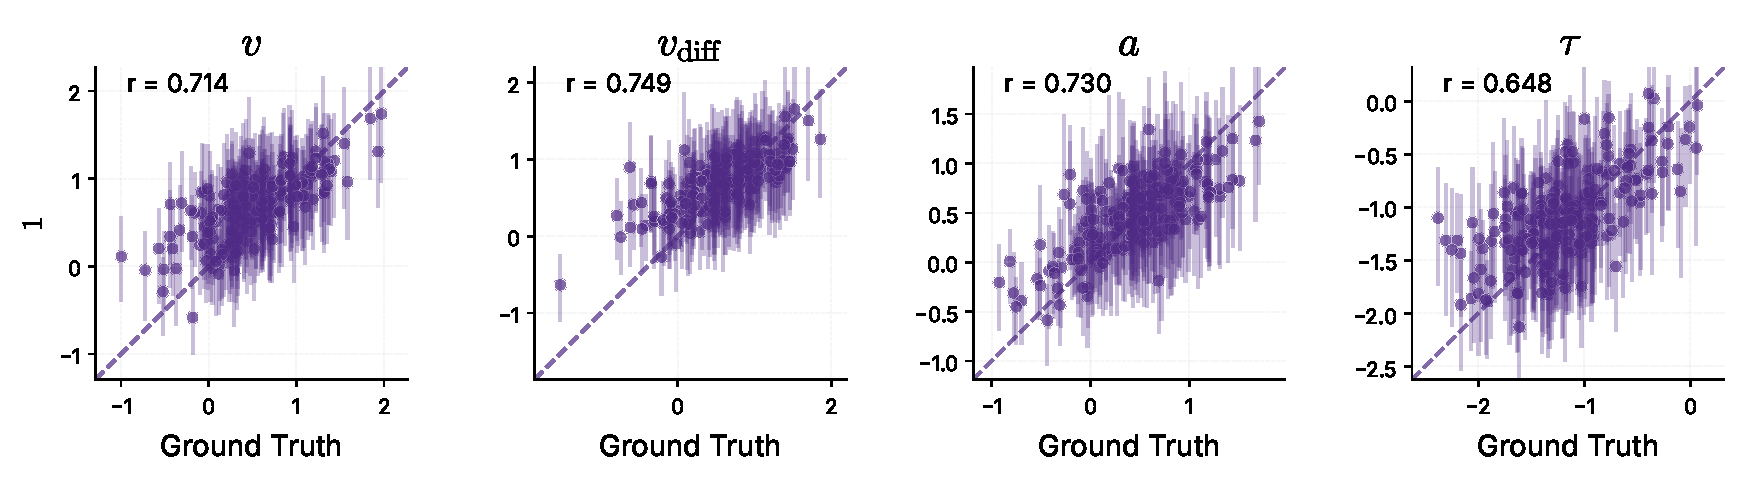
\includegraphics[width=\linewidth,height=0.84\textheight,keepaspectratio]{finetuned/lba/fixed/recovery.pdf}
  \caption[LBA, fixed, finetuned: recovery]{\textbf{LBA, fixed design, finetuned --- coefficient recovery.} Posterior mean (points) with 95\% credible intervals against the
    data-generating value, one panel per active cell of the coefficient matrix
    $\mathbf{B}$. Columns are intrinsic parameters, rows are design columns
    (intercept, main effects, interactions), labeled by regressor and category;
    the panel axes render this as \texttt{predictor|category}. Inactive cells are
    drawn as grey N/A tiles. Point color encodes the row kind: intercept (purple),
    main effect (blue), interaction (red). This arm evaluates the LBA-finetuned checkpoint.}
  \label{fig:e3-lba-fixed-finetuned-rec}
\end{figure}

\begin{figure}[htbp]
  \centering
  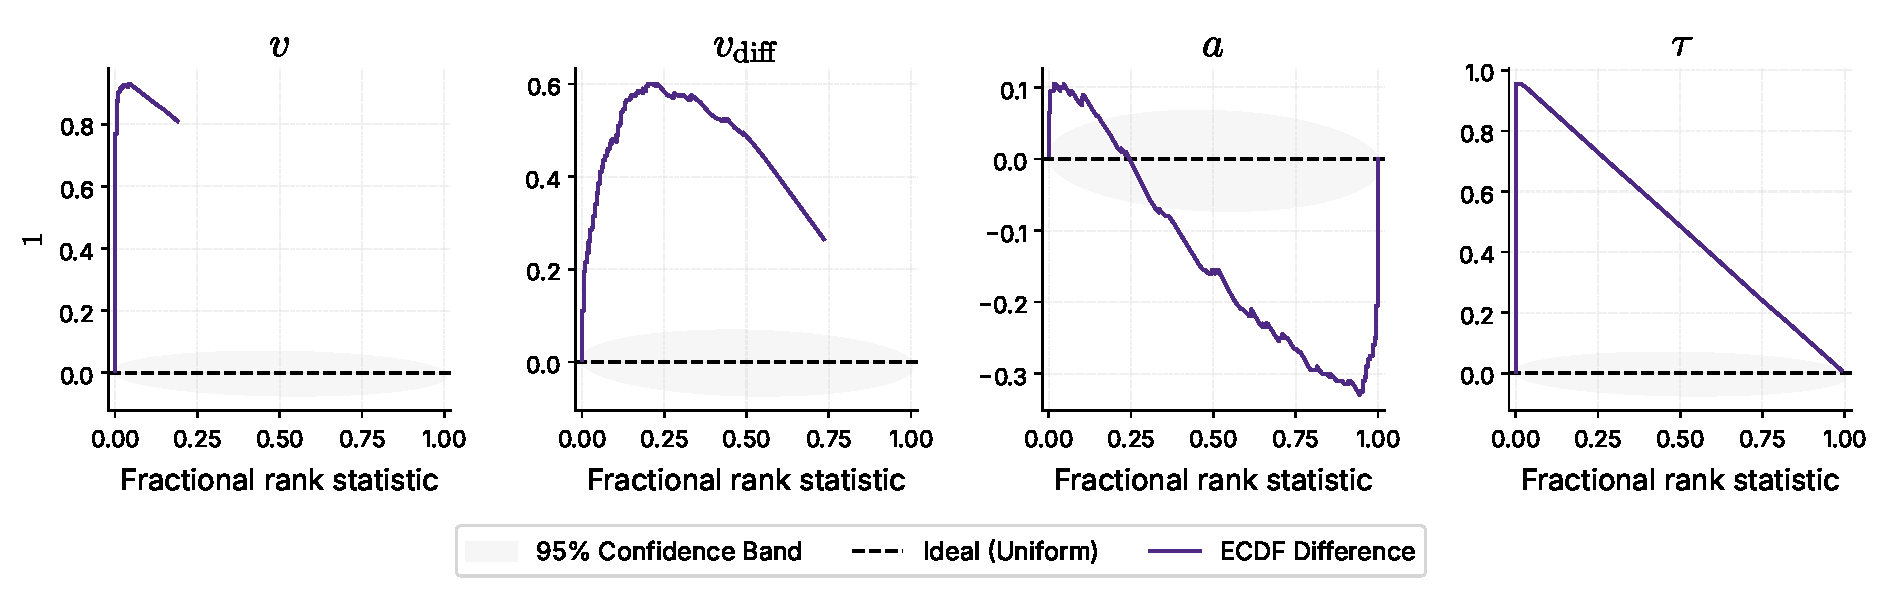
\includegraphics[width=\linewidth,height=0.84\textheight,keepaspectratio]{zeroshot/lba/fixed/ecdf.pdf}
  \caption[LBA, fixed, zero-shot: ECDF calibration]{\textbf{LBA, fixed design, zero-shot --- ECDF calibration.} Rank-ECDF difference (empirical minus uniform) with simultaneous
    95\% confidence bands, on the same cell layout as the corresponding recovery
    figure (Figure~\ref{fig:e3-lba-fixed-zeroshot-rec}). A calibrated posterior stays inside the band;
    excursions above/below indicate bias, and a systematically shallow/steep curve
    indicates over-/under-dispersion.}
  \label{fig:e3-lba-fixed-zeroshot-ecdf}
\end{figure}

\begin{figure}[htbp]
  \centering
  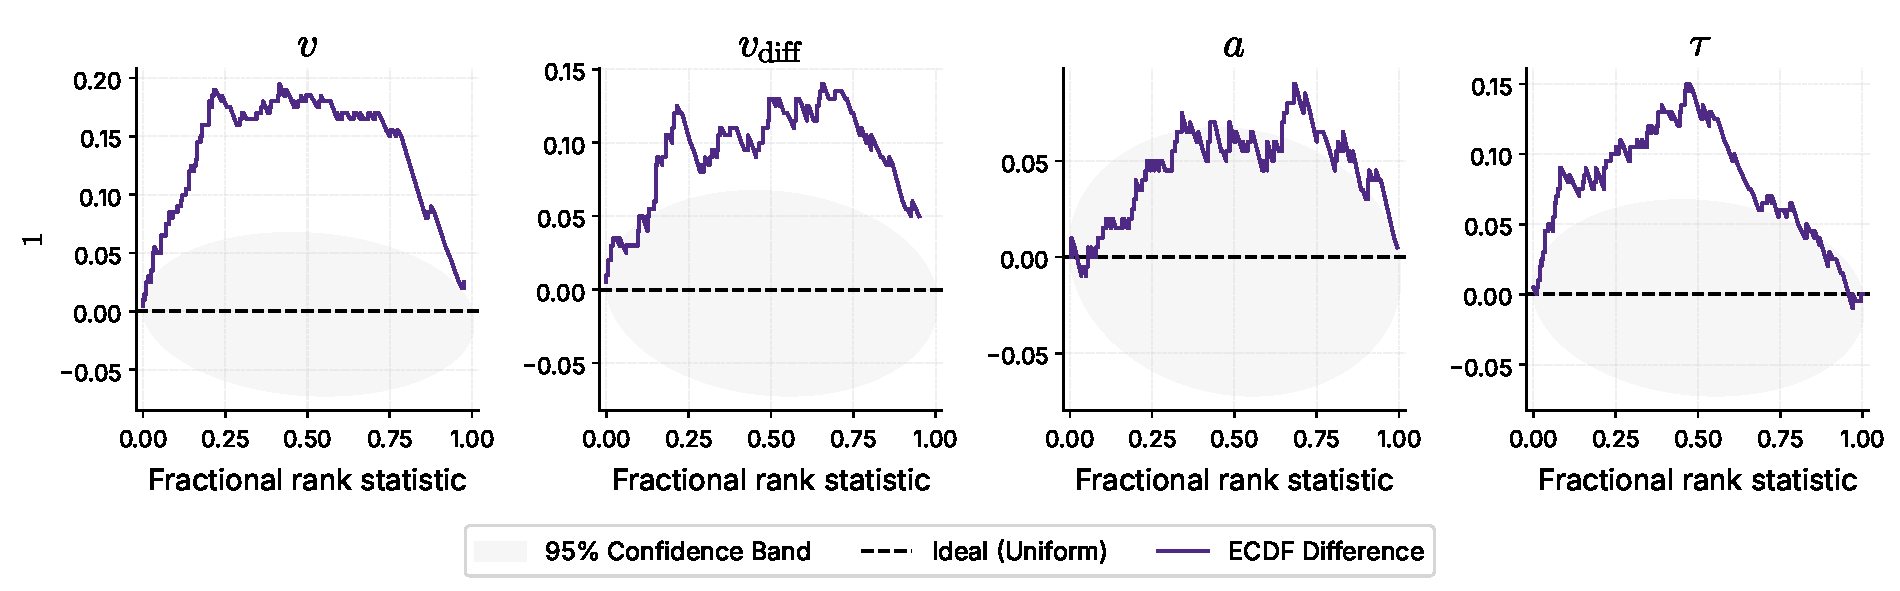
\includegraphics[width=\linewidth,height=0.84\textheight,keepaspectratio]{finetuned/lba/fixed/ecdf.pdf}
  \caption[LBA, fixed, finetuned: ECDF calibration]{\textbf{LBA, fixed design, finetuned --- ECDF calibration.} Rank-ECDF difference (empirical minus uniform) with simultaneous
    95\% confidence bands, on the same cell layout as the corresponding recovery
    figure (Figure~\ref{fig:e3-lba-fixed-finetuned-rec}). A calibrated posterior stays inside the band;
    excursions above/below indicate bias, and a systematically shallow/steep curve
    indicates over-/under-dispersion.}
  \label{fig:e3-lba-fixed-finetuned-ecdf}
\end{figure}

\FloatBarrier
\clearpage

%-----------------------------------------------------------------------------
\subsection{LBA, mixed-predictor design}
\label{sec:e3-lba-mixed_predictor}
%-----------------------------------------------------------------------------

\begin{figure}[htbp]
  \centering
  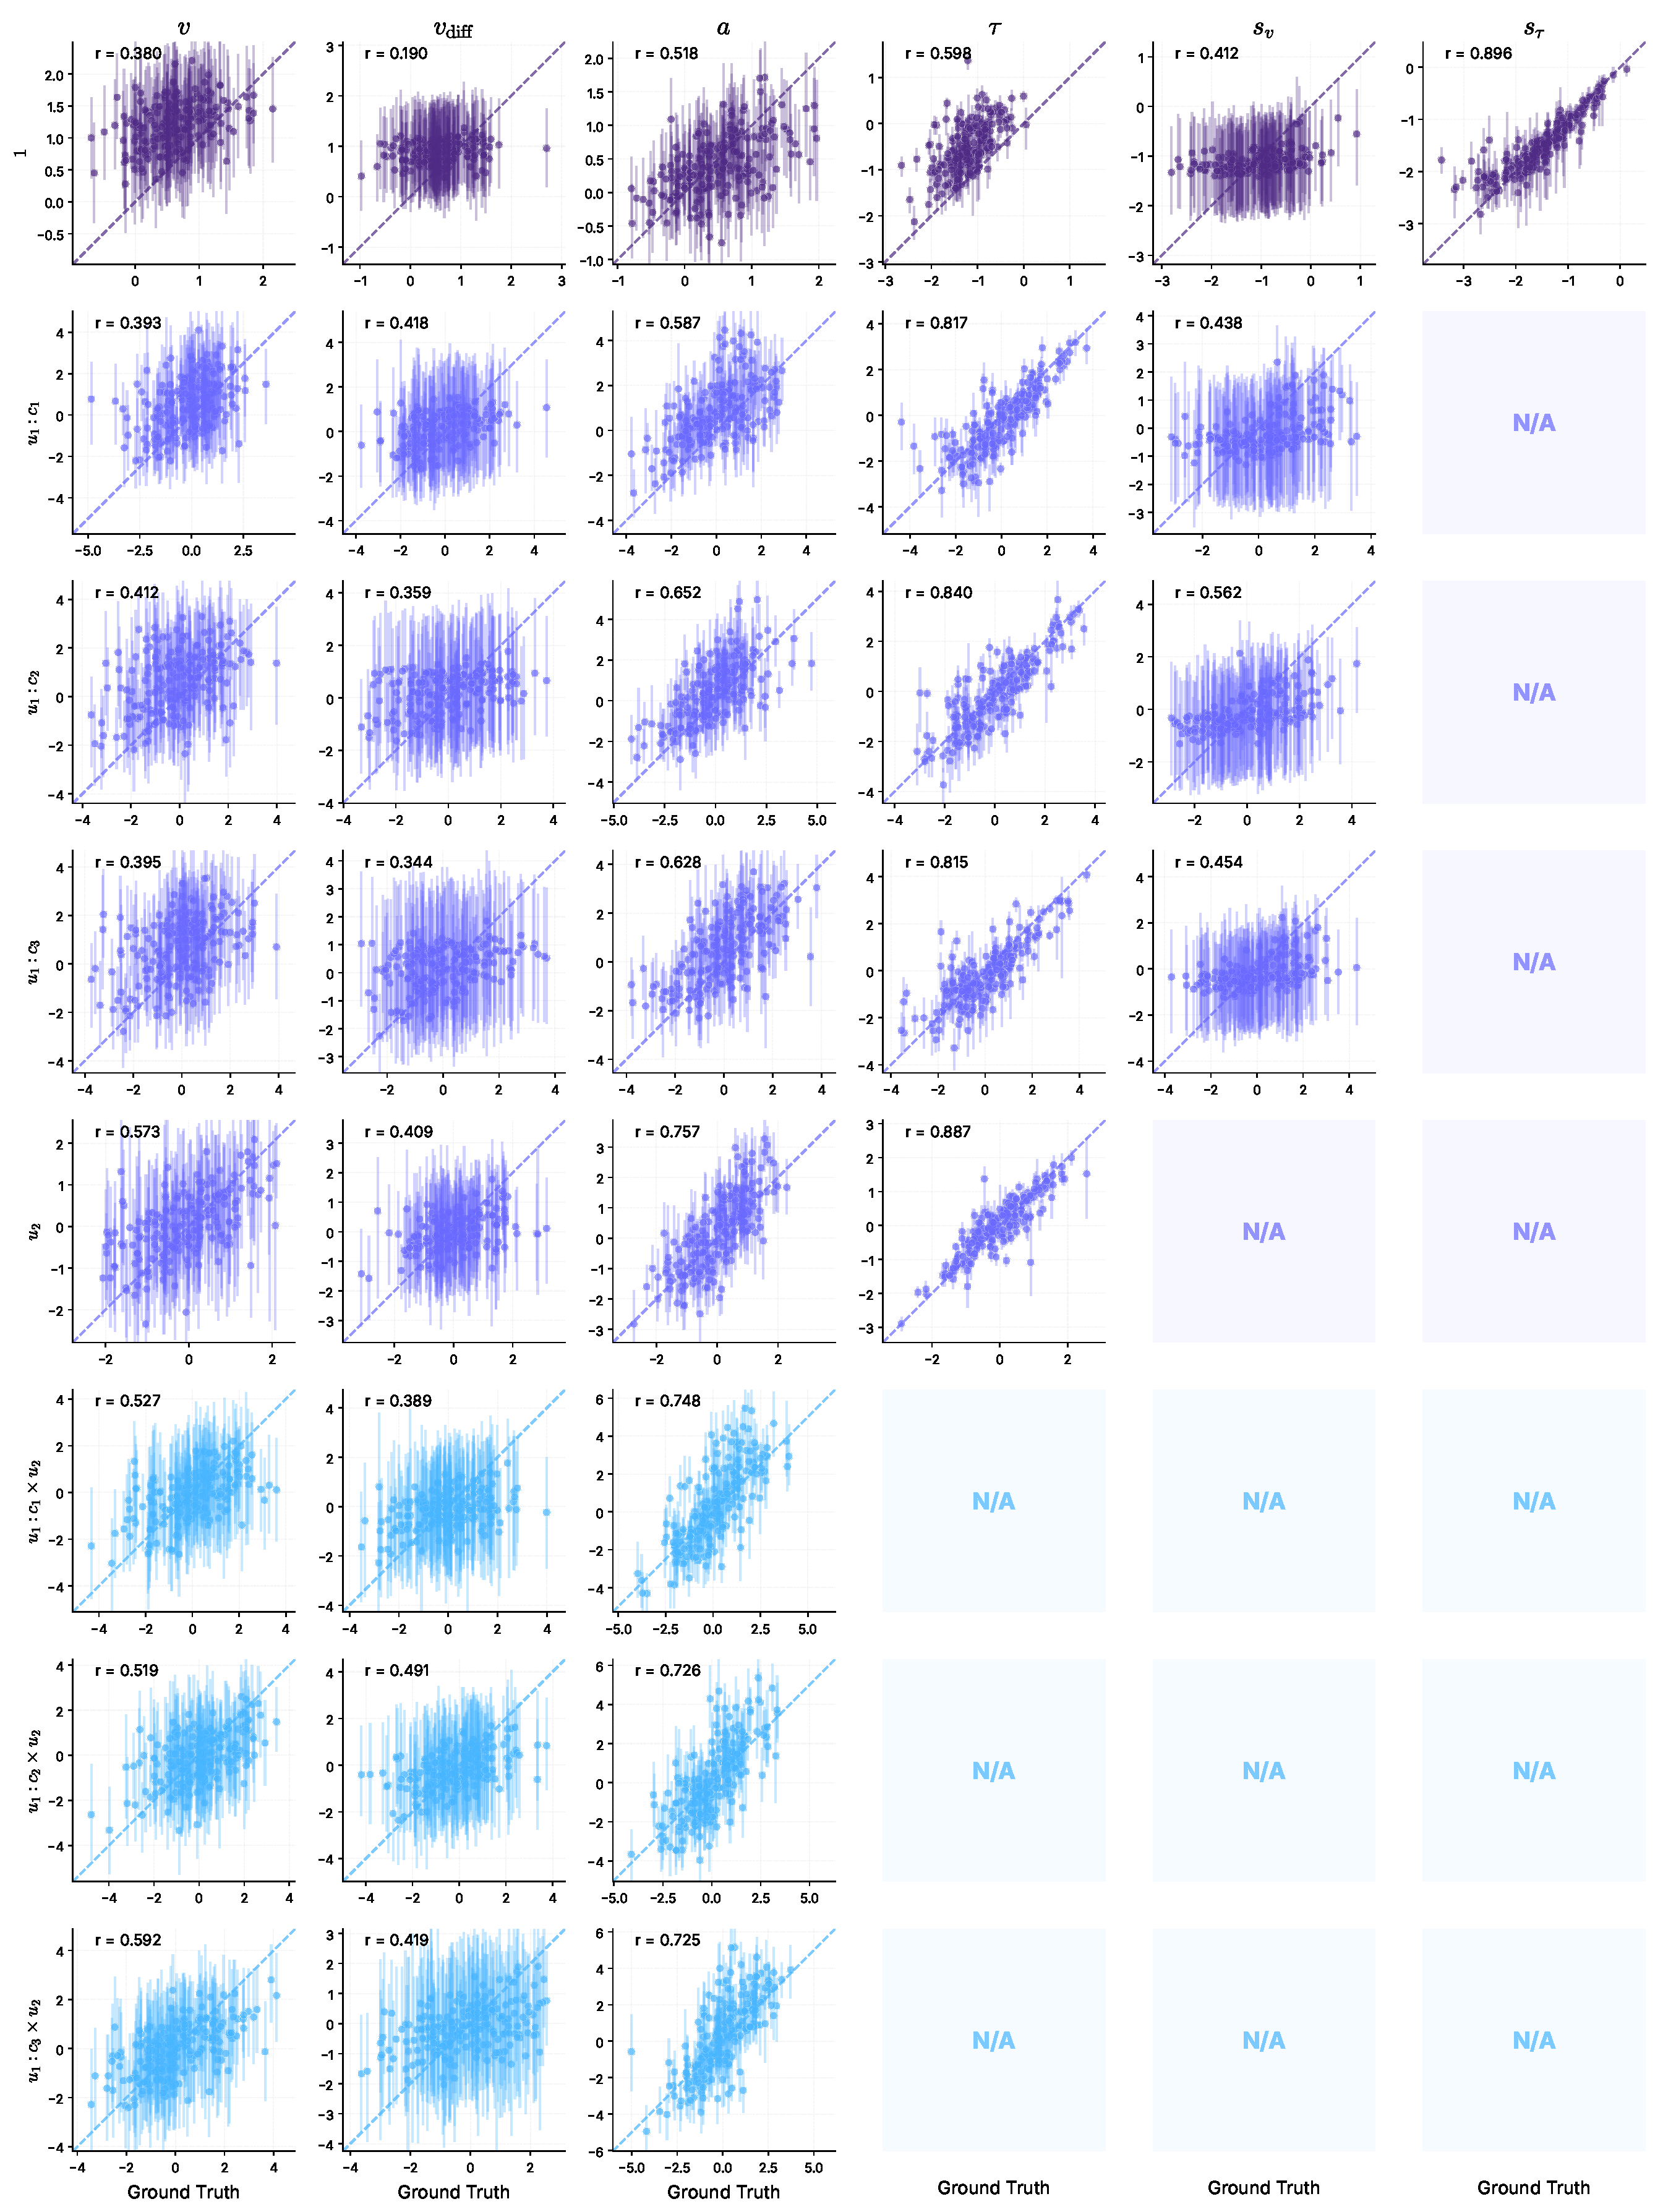
\includegraphics[width=\linewidth,height=0.84\textheight,keepaspectratio]{zeroshot/lba/mixed_predictor/recovery.pdf}
  \caption[LBA, mixed-predictor, zero-shot: recovery]{\textbf{LBA, mixed-predictor design, zero-shot --- coefficient recovery.} Posterior mean (points) with 95\% credible intervals against the
    data-generating value, one panel per active cell of the coefficient matrix
    $\mathbf{B}$. Columns are intrinsic parameters, rows are design columns
    (intercept, main effects, interactions), labeled by regressor and category;
    the panel axes render this as \texttt{predictor|category}. Inactive cells are
    drawn as grey N/A tiles. Point color encodes the row kind: intercept (purple),
    main effect (blue), interaction (red). This arm evaluates the original pre-finetune checkpoint applied to LBA without any LBA training.}
  \label{fig:e3-lba-mixed_predictor-zeroshot-rec}
\end{figure}

\begin{figure}[htbp]
  \centering
  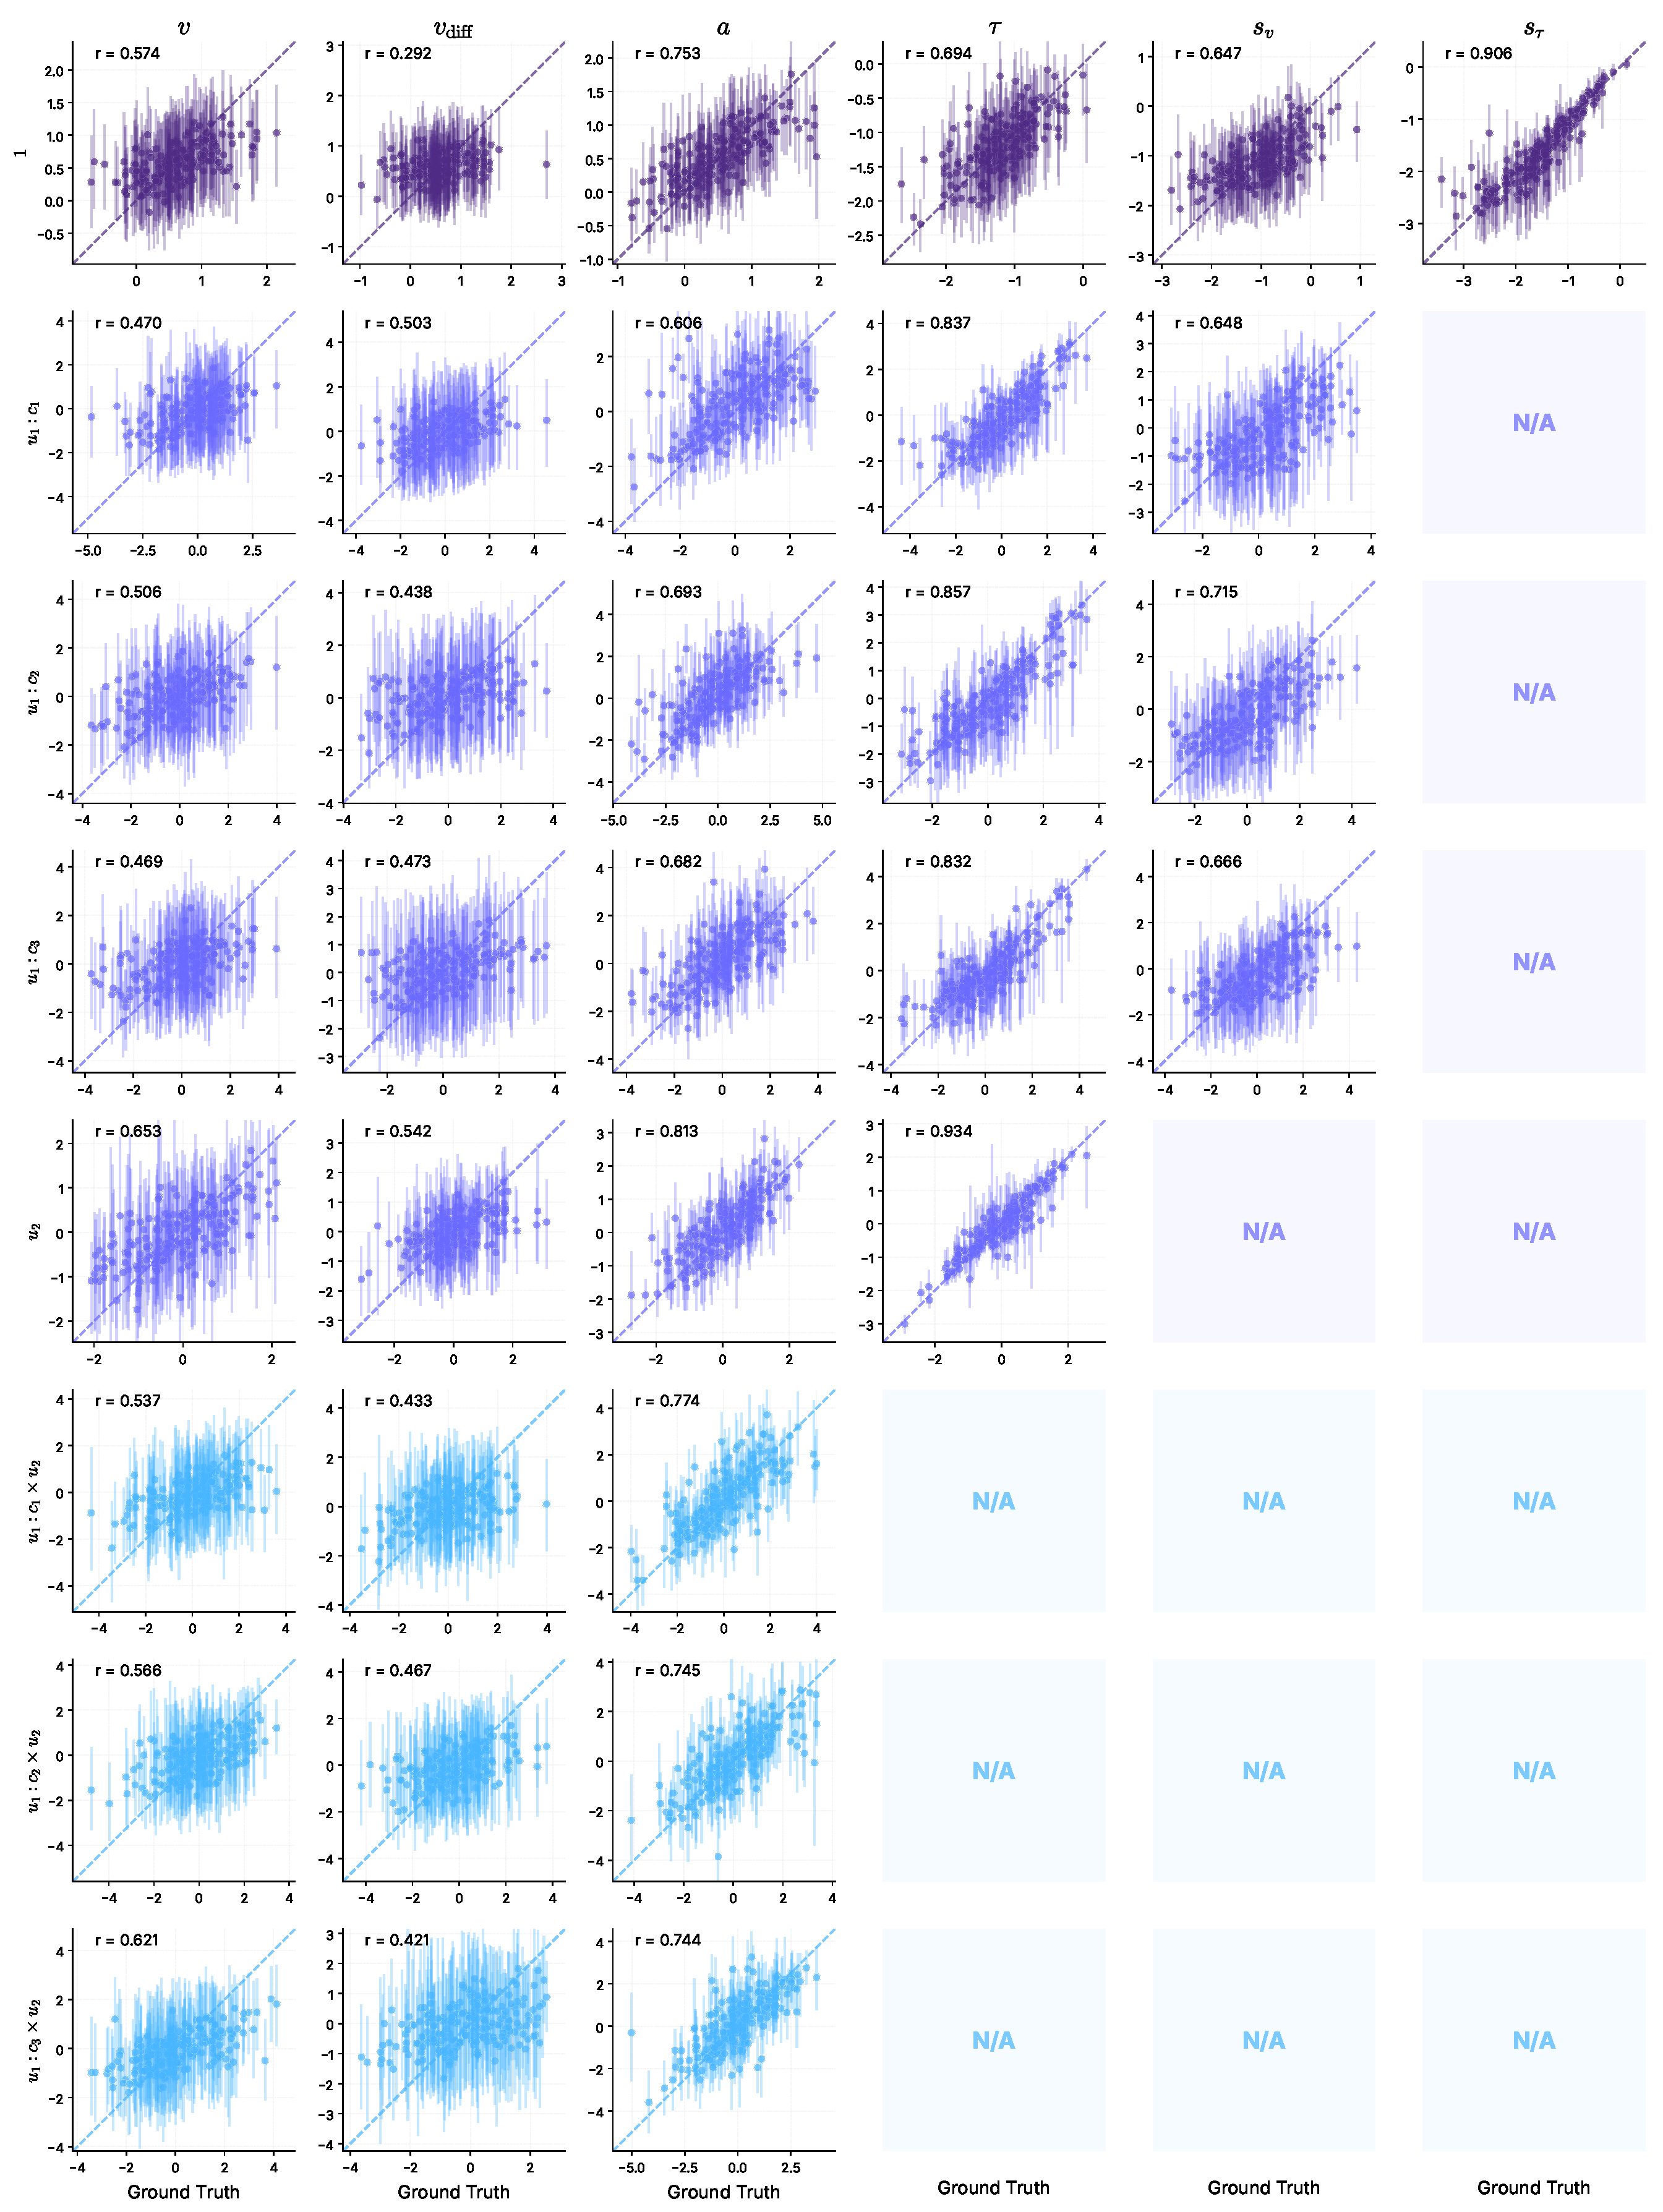
\includegraphics[width=\linewidth,height=0.84\textheight,keepaspectratio]{finetuned/lba/mixed_predictor/recovery.pdf}
  \caption[LBA, mixed-predictor, finetuned: recovery]{\textbf{LBA, mixed-predictor design, finetuned --- coefficient recovery.} Posterior mean (points) with 95\% credible intervals against the
    data-generating value, one panel per active cell of the coefficient matrix
    $\mathbf{B}$. Columns are intrinsic parameters, rows are design columns
    (intercept, main effects, interactions), labeled by regressor and category;
    the panel axes render this as \texttt{predictor|category}. Inactive cells are
    drawn as grey N/A tiles. Point color encodes the row kind: intercept (purple),
    main effect (blue), interaction (red). This arm evaluates the LBA-finetuned checkpoint.}
  \label{fig:e3-lba-mixed_predictor-finetuned-rec}
\end{figure}

\begin{figure}[htbp]
  \centering
  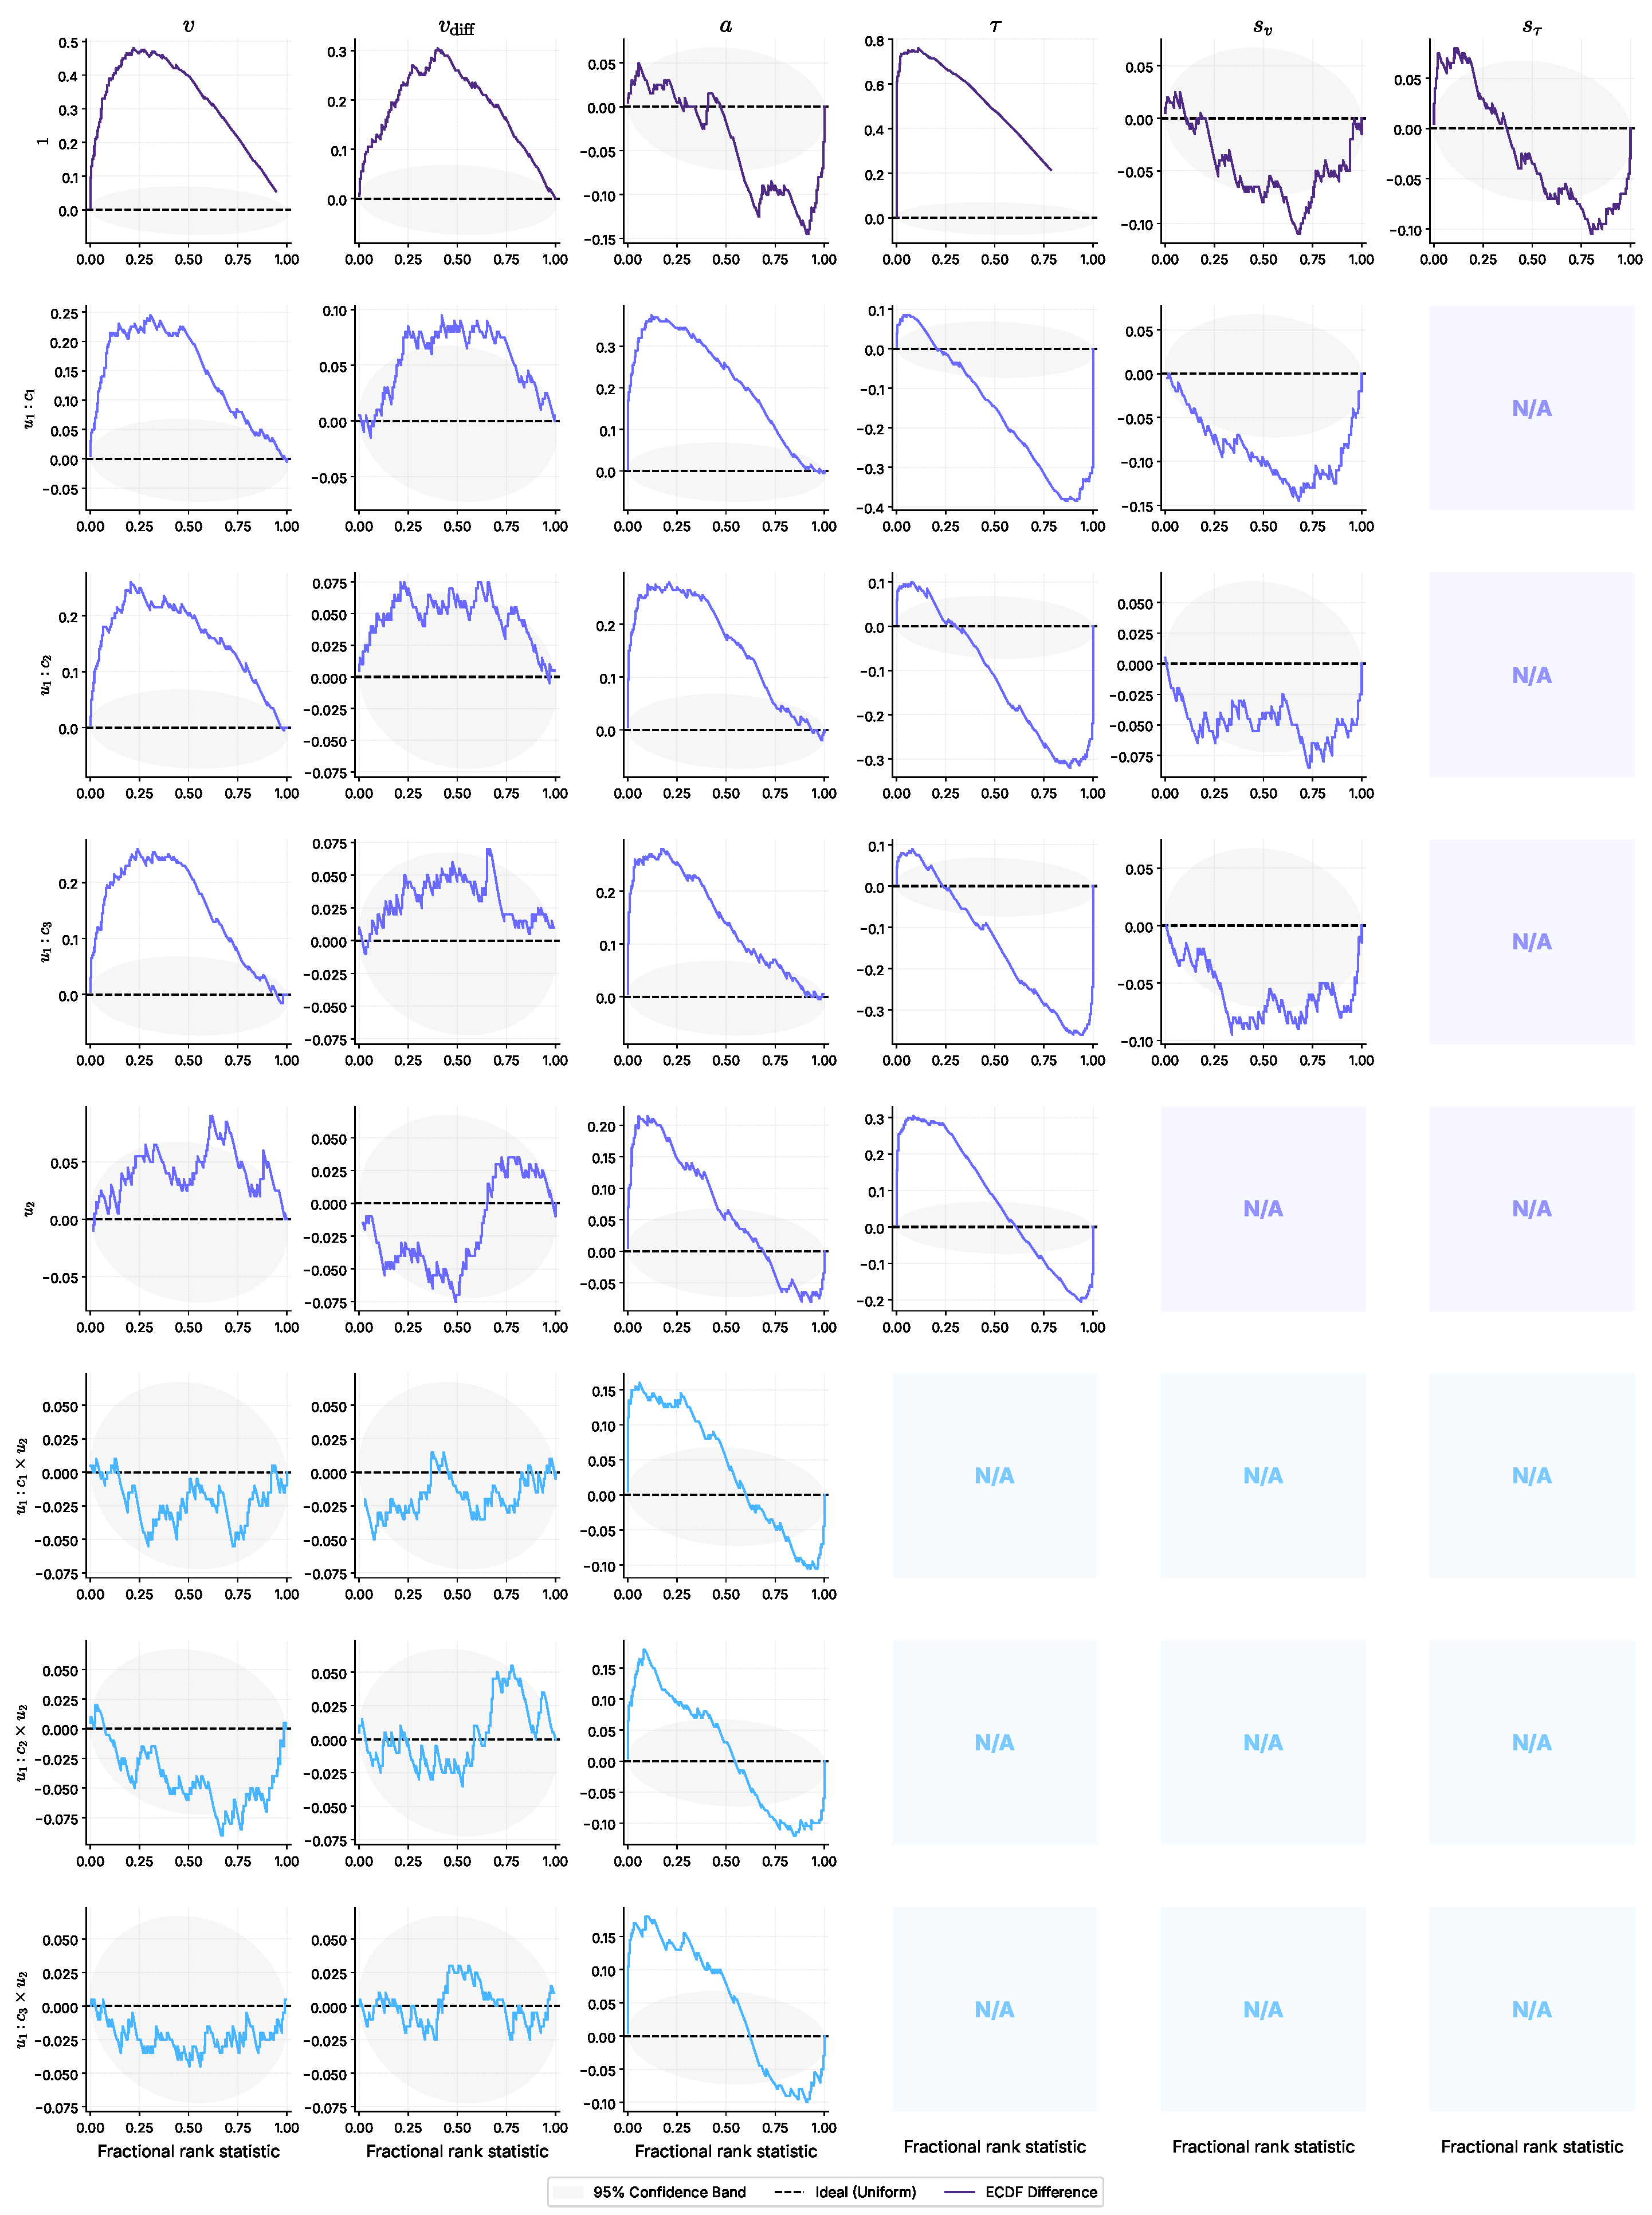
\includegraphics[width=\linewidth,height=0.84\textheight,keepaspectratio]{zeroshot/lba/mixed_predictor/ecdf.pdf}
  \caption[LBA, mixed-predictor, zero-shot: ECDF calibration]{\textbf{LBA, mixed-predictor design, zero-shot --- ECDF calibration.} Rank-ECDF difference (empirical minus uniform) with simultaneous
    95\% confidence bands, on the same cell layout as the corresponding recovery
    figure (Figure~\ref{fig:e3-lba-mixed_predictor-zeroshot-rec}). A calibrated posterior stays inside the band;
    excursions above/below indicate bias, and a systematically shallow/steep curve
    indicates over-/under-dispersion.}
  \label{fig:e3-lba-mixed_predictor-zeroshot-ecdf}
\end{figure}

\begin{figure}[htbp]
  \centering
  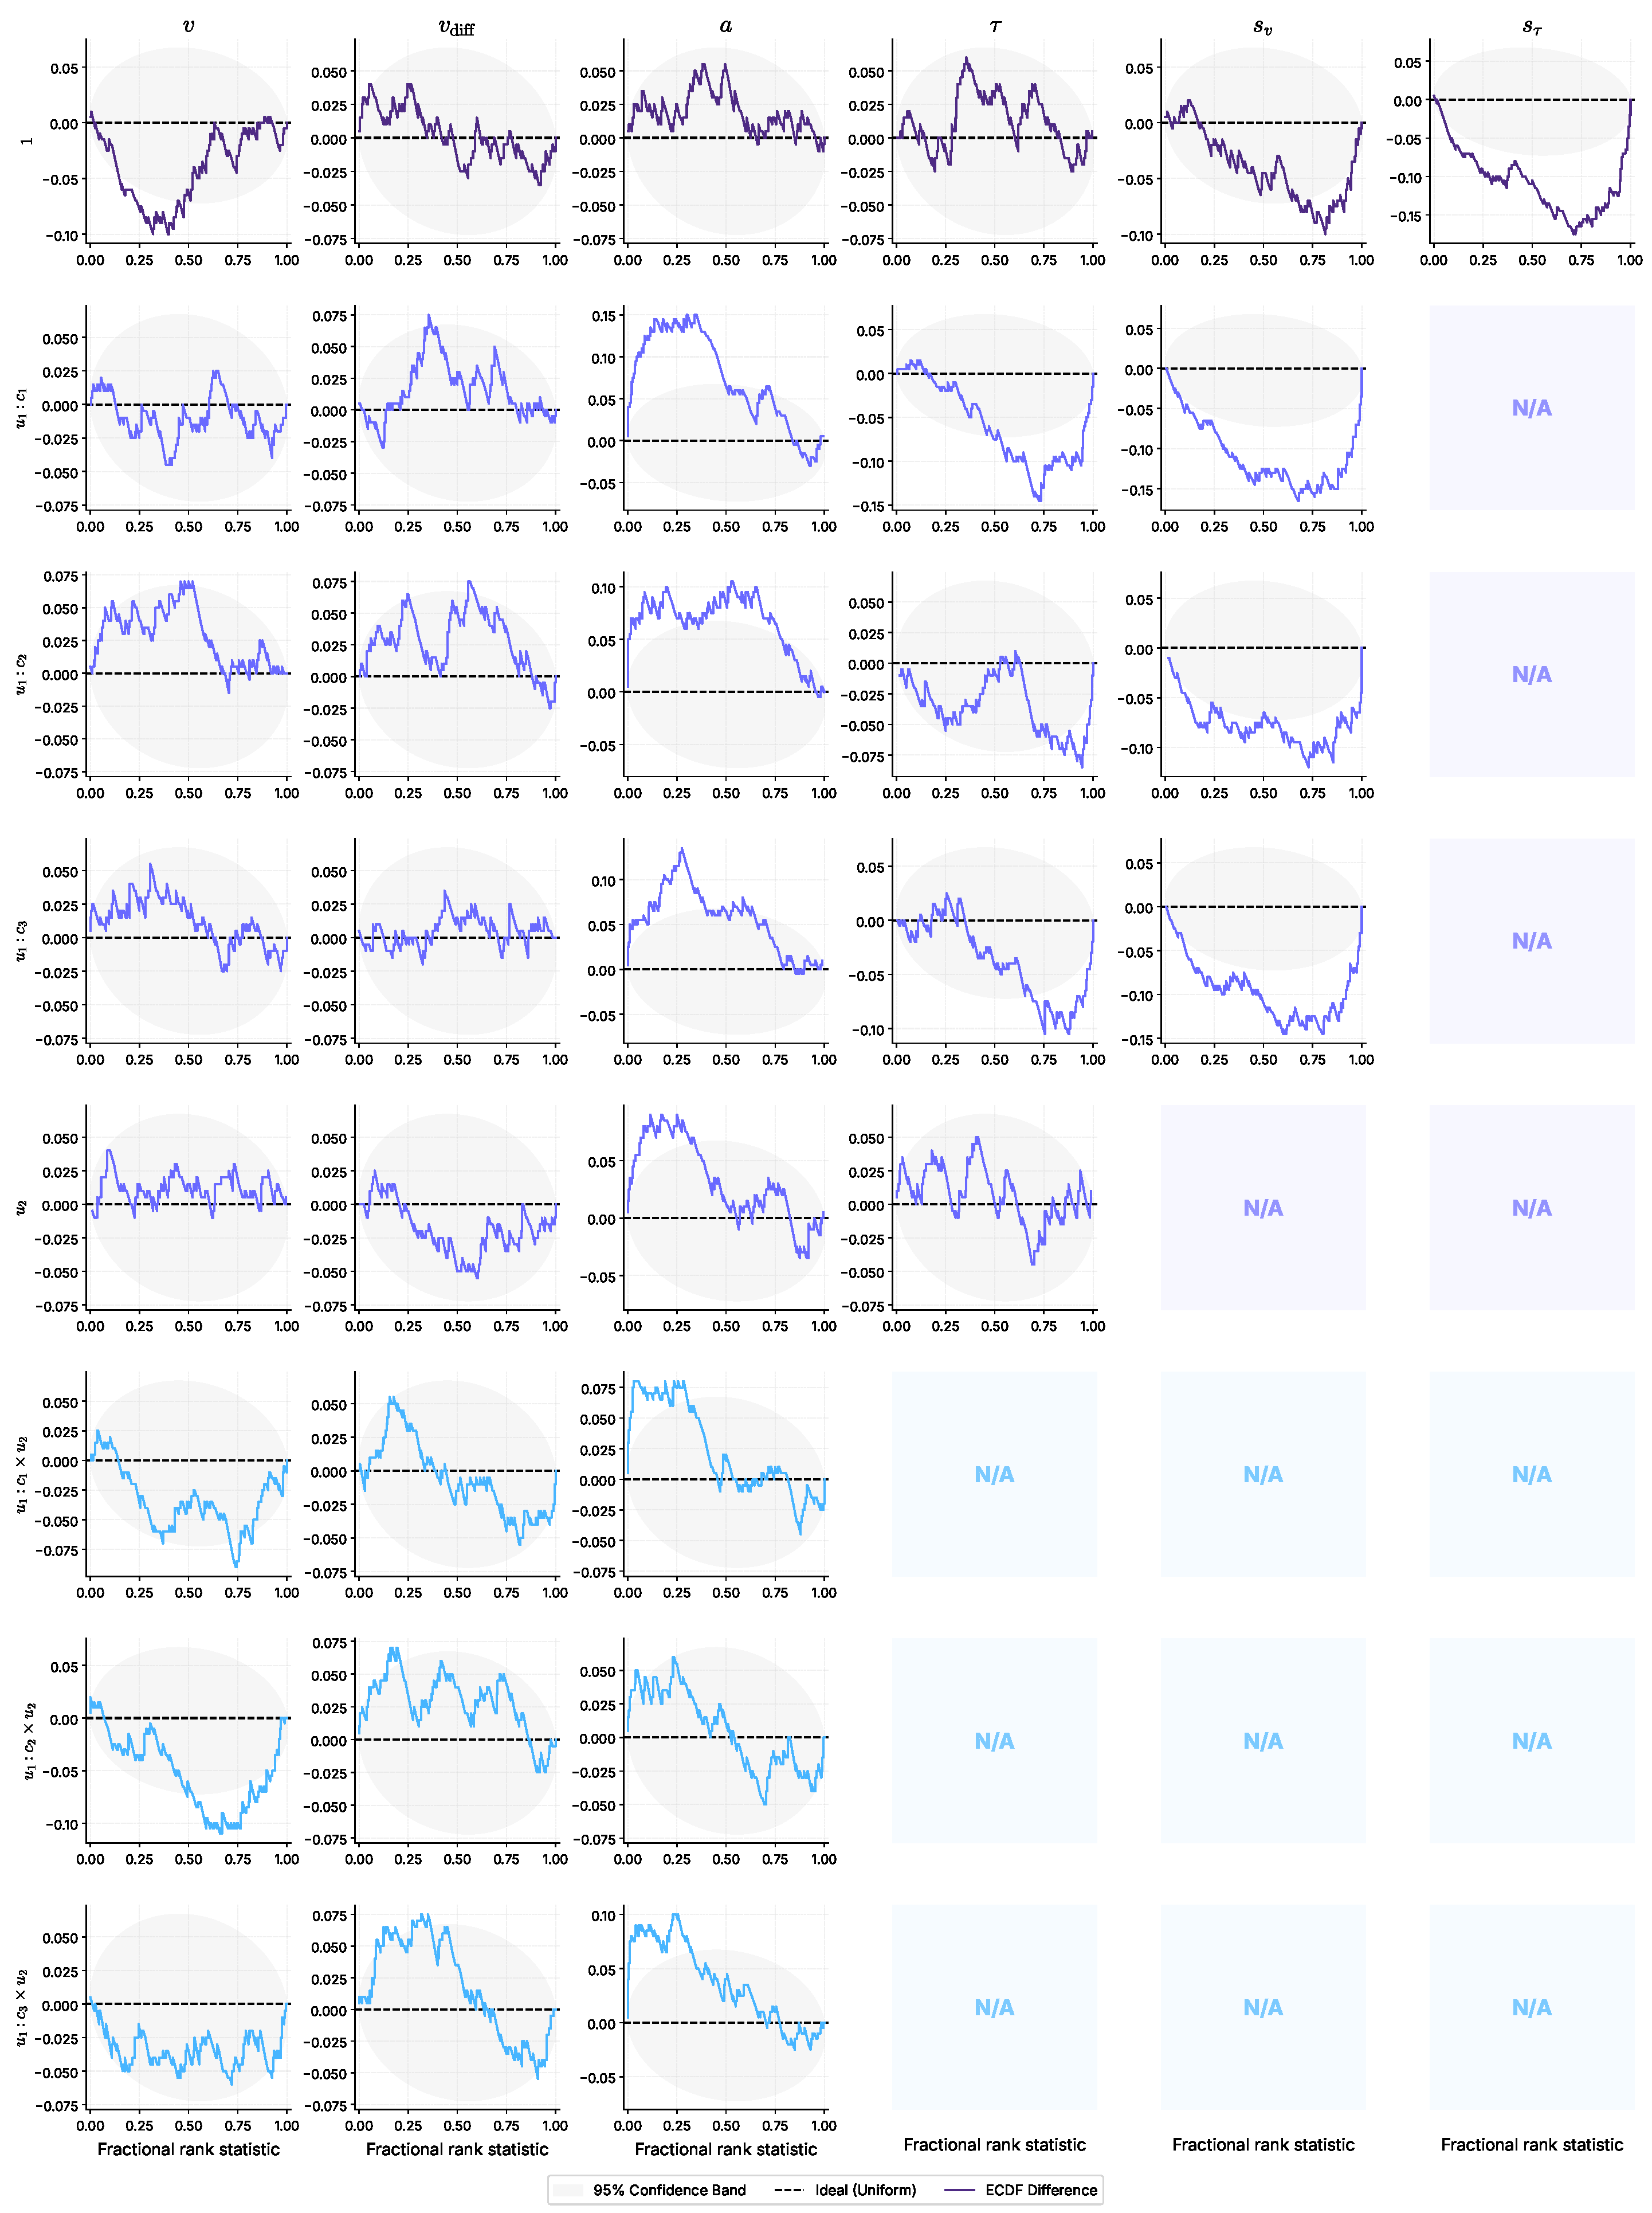
\includegraphics[width=\linewidth,height=0.84\textheight,keepaspectratio]{finetuned/lba/mixed_predictor/ecdf.pdf}
  \caption[LBA, mixed-predictor, finetuned: ECDF calibration]{\textbf{LBA, mixed-predictor design, finetuned --- ECDF calibration.} Rank-ECDF difference (empirical minus uniform) with simultaneous
    95\% confidence bands, on the same cell layout as the corresponding recovery
    figure (Figure~\ref{fig:e3-lba-mixed_predictor-finetuned-rec}). A calibrated posterior stays inside the band;
    excursions above/below indicate bias, and a systematically shallow/steep curve
    indicates over-/under-dispersion.}
  \label{fig:e3-lba-mixed_predictor-finetuned-ecdf}
\end{figure}

\FloatBarrier

% --- Restore LaTeX default float parameters -----------------------------------
\renewcommand{\topfraction}{0.7}
\renewcommand{\bottomfraction}{0.3}
\renewcommand{\textfraction}{0.2}
\renewcommand{\floatpagefraction}{0.5}

%=============================================================================
% END OF EXPERIMENT 3 APPENDIX SECTION (LBA arms)
%=============================================================================
